% Options for packages loaded elsewhere
\PassOptionsToPackage{unicode}{hyperref}
\PassOptionsToPackage{hyphens}{url}
\PassOptionsToPackage{dvipsnames,svgnames,x11names}{xcolor}
%
\documentclass[
  letterpaper,
  DIV=11,
  numbers=noendperiod]{scrartcl}

\usepackage{amsmath,amssymb}
\usepackage{iftex}
\ifPDFTeX
  \usepackage[T1]{fontenc}
  \usepackage[utf8]{inputenc}
  \usepackage{textcomp} % provide euro and other symbols
\else % if luatex or xetex
  \usepackage{unicode-math}
  \defaultfontfeatures{Scale=MatchLowercase}
  \defaultfontfeatures[\rmfamily]{Ligatures=TeX,Scale=1}
\fi
\usepackage{lmodern}
\ifPDFTeX\else  
    % xetex/luatex font selection
\fi
% Use upquote if available, for straight quotes in verbatim environments
\IfFileExists{upquote.sty}{\usepackage{upquote}}{}
\IfFileExists{microtype.sty}{% use microtype if available
  \usepackage[]{microtype}
  \UseMicrotypeSet[protrusion]{basicmath} % disable protrusion for tt fonts
}{}
\makeatletter
\@ifundefined{KOMAClassName}{% if non-KOMA class
  \IfFileExists{parskip.sty}{%
    \usepackage{parskip}
  }{% else
    \setlength{\parindent}{0pt}
    \setlength{\parskip}{6pt plus 2pt minus 1pt}}
}{% if KOMA class
  \KOMAoptions{parskip=half}}
\makeatother
\usepackage{xcolor}
\setlength{\emergencystretch}{3em} % prevent overfull lines
\setcounter{secnumdepth}{-\maxdimen} % remove section numbering
% Make \paragraph and \subparagraph free-standing
\ifx\paragraph\undefined\else
  \let\oldparagraph\paragraph
  \renewcommand{\paragraph}[1]{\oldparagraph{#1}\mbox{}}
\fi
\ifx\subparagraph\undefined\else
  \let\oldsubparagraph\subparagraph
  \renewcommand{\subparagraph}[1]{\oldsubparagraph{#1}\mbox{}}
\fi

\usepackage{color}
\usepackage{fancyvrb}
\newcommand{\VerbBar}{|}
\newcommand{\VERB}{\Verb[commandchars=\\\{\}]}
\DefineVerbatimEnvironment{Highlighting}{Verbatim}{commandchars=\\\{\}}
% Add ',fontsize=\small' for more characters per line
\usepackage{framed}
\definecolor{shadecolor}{RGB}{241,243,245}
\newenvironment{Shaded}{\begin{snugshade}}{\end{snugshade}}
\newcommand{\AlertTok}[1]{\textcolor[rgb]{0.68,0.00,0.00}{#1}}
\newcommand{\AnnotationTok}[1]{\textcolor[rgb]{0.37,0.37,0.37}{#1}}
\newcommand{\AttributeTok}[1]{\textcolor[rgb]{0.40,0.45,0.13}{#1}}
\newcommand{\BaseNTok}[1]{\textcolor[rgb]{0.68,0.00,0.00}{#1}}
\newcommand{\BuiltInTok}[1]{\textcolor[rgb]{0.00,0.23,0.31}{#1}}
\newcommand{\CharTok}[1]{\textcolor[rgb]{0.13,0.47,0.30}{#1}}
\newcommand{\CommentTok}[1]{\textcolor[rgb]{0.37,0.37,0.37}{#1}}
\newcommand{\CommentVarTok}[1]{\textcolor[rgb]{0.37,0.37,0.37}{\textit{#1}}}
\newcommand{\ConstantTok}[1]{\textcolor[rgb]{0.56,0.35,0.01}{#1}}
\newcommand{\ControlFlowTok}[1]{\textcolor[rgb]{0.00,0.23,0.31}{#1}}
\newcommand{\DataTypeTok}[1]{\textcolor[rgb]{0.68,0.00,0.00}{#1}}
\newcommand{\DecValTok}[1]{\textcolor[rgb]{0.68,0.00,0.00}{#1}}
\newcommand{\DocumentationTok}[1]{\textcolor[rgb]{0.37,0.37,0.37}{\textit{#1}}}
\newcommand{\ErrorTok}[1]{\textcolor[rgb]{0.68,0.00,0.00}{#1}}
\newcommand{\ExtensionTok}[1]{\textcolor[rgb]{0.00,0.23,0.31}{#1}}
\newcommand{\FloatTok}[1]{\textcolor[rgb]{0.68,0.00,0.00}{#1}}
\newcommand{\FunctionTok}[1]{\textcolor[rgb]{0.28,0.35,0.67}{#1}}
\newcommand{\ImportTok}[1]{\textcolor[rgb]{0.00,0.46,0.62}{#1}}
\newcommand{\InformationTok}[1]{\textcolor[rgb]{0.37,0.37,0.37}{#1}}
\newcommand{\KeywordTok}[1]{\textcolor[rgb]{0.00,0.23,0.31}{#1}}
\newcommand{\NormalTok}[1]{\textcolor[rgb]{0.00,0.23,0.31}{#1}}
\newcommand{\OperatorTok}[1]{\textcolor[rgb]{0.37,0.37,0.37}{#1}}
\newcommand{\OtherTok}[1]{\textcolor[rgb]{0.00,0.23,0.31}{#1}}
\newcommand{\PreprocessorTok}[1]{\textcolor[rgb]{0.68,0.00,0.00}{#1}}
\newcommand{\RegionMarkerTok}[1]{\textcolor[rgb]{0.00,0.23,0.31}{#1}}
\newcommand{\SpecialCharTok}[1]{\textcolor[rgb]{0.37,0.37,0.37}{#1}}
\newcommand{\SpecialStringTok}[1]{\textcolor[rgb]{0.13,0.47,0.30}{#1}}
\newcommand{\StringTok}[1]{\textcolor[rgb]{0.13,0.47,0.30}{#1}}
\newcommand{\VariableTok}[1]{\textcolor[rgb]{0.07,0.07,0.07}{#1}}
\newcommand{\VerbatimStringTok}[1]{\textcolor[rgb]{0.13,0.47,0.30}{#1}}
\newcommand{\WarningTok}[1]{\textcolor[rgb]{0.37,0.37,0.37}{\textit{#1}}}

\providecommand{\tightlist}{%
  \setlength{\itemsep}{0pt}\setlength{\parskip}{0pt}}\usepackage{longtable,booktabs,array}
\usepackage{calc} % for calculating minipage widths
% Correct order of tables after \paragraph or \subparagraph
\usepackage{etoolbox}
\makeatletter
\patchcmd\longtable{\par}{\if@noskipsec\mbox{}\fi\par}{}{}
\makeatother
% Allow footnotes in longtable head/foot
\IfFileExists{footnotehyper.sty}{\usepackage{footnotehyper}}{\usepackage{footnote}}
\makesavenoteenv{longtable}
\usepackage{graphicx}
\makeatletter
\def\maxwidth{\ifdim\Gin@nat@width>\linewidth\linewidth\else\Gin@nat@width\fi}
\def\maxheight{\ifdim\Gin@nat@height>\textheight\textheight\else\Gin@nat@height\fi}
\makeatother
% Scale images if necessary, so that they will not overflow the page
% margins by default, and it is still possible to overwrite the defaults
% using explicit options in \includegraphics[width, height, ...]{}
\setkeys{Gin}{width=\maxwidth,height=\maxheight,keepaspectratio}
% Set default figure placement to htbp
\makeatletter
\def\fps@figure{htbp}
\makeatother

\KOMAoption{captions}{tableheading}
\makeatletter
\@ifpackageloaded{tcolorbox}{}{\usepackage[skins,breakable]{tcolorbox}}
\@ifpackageloaded{fontawesome5}{}{\usepackage{fontawesome5}}
\definecolor{quarto-callout-color}{HTML}{909090}
\definecolor{quarto-callout-note-color}{HTML}{0758E5}
\definecolor{quarto-callout-important-color}{HTML}{CC1914}
\definecolor{quarto-callout-warning-color}{HTML}{EB9113}
\definecolor{quarto-callout-tip-color}{HTML}{00A047}
\definecolor{quarto-callout-caution-color}{HTML}{FC5300}
\definecolor{quarto-callout-color-frame}{HTML}{acacac}
\definecolor{quarto-callout-note-color-frame}{HTML}{4582ec}
\definecolor{quarto-callout-important-color-frame}{HTML}{d9534f}
\definecolor{quarto-callout-warning-color-frame}{HTML}{f0ad4e}
\definecolor{quarto-callout-tip-color-frame}{HTML}{02b875}
\definecolor{quarto-callout-caution-color-frame}{HTML}{fd7e14}
\makeatother
\makeatletter
\@ifpackageloaded{caption}{}{\usepackage{caption}}
\AtBeginDocument{%
\ifdefined\contentsname
  \renewcommand*\contentsname{Table of contents}
\else
  \newcommand\contentsname{Table of contents}
\fi
\ifdefined\listfigurename
  \renewcommand*\listfigurename{List of Figures}
\else
  \newcommand\listfigurename{List of Figures}
\fi
\ifdefined\listtablename
  \renewcommand*\listtablename{List of Tables}
\else
  \newcommand\listtablename{List of Tables}
\fi
\ifdefined\figurename
  \renewcommand*\figurename{Figure}
\else
  \newcommand\figurename{Figure}
\fi
\ifdefined\tablename
  \renewcommand*\tablename{Table}
\else
  \newcommand\tablename{Table}
\fi
}
\@ifpackageloaded{float}{}{\usepackage{float}}
\floatstyle{ruled}
\@ifundefined{c@chapter}{\newfloat{codelisting}{h}{lop}}{\newfloat{codelisting}{h}{lop}[chapter]}
\floatname{codelisting}{Listing}
\newcommand*\listoflistings{\listof{codelisting}{List of Listings}}
\makeatother
\makeatletter
\makeatother
\makeatletter
\@ifpackageloaded{caption}{}{\usepackage{caption}}
\@ifpackageloaded{subcaption}{}{\usepackage{subcaption}}
\makeatother
\ifLuaTeX
  \usepackage{selnolig}  % disable illegal ligatures
\fi
\usepackage{bookmark}

\IfFileExists{xurl.sty}{\usepackage{xurl}}{} % add URL line breaks if available
\urlstyle{same} % disable monospaced font for URLs
\hypersetup{
  pdftitle={Levantamiento GNSS con receptor AllyNav R26: ocupación estática de punto geodésico y levantamiento RTK de borde de vía},
  pdfauthor={Fernan Jose Severich Diaz (Teoría y Práctica), Raul Andrés Posada (Teoría)},
  colorlinks=true,
  linkcolor={blue},
  filecolor={Maroon},
  citecolor={Blue},
  urlcolor={Blue},
  pdfcreator={LaTeX via pandoc}}

\title{Levantamiento GNSS con receptor AllyNav R26: ocupación estática
de punto geodésico y levantamiento RTK de borde de vía}
\author{Fernan Jose Severich Diaz (Teoría y Práctica), Raul Andrés
Posada (Teoría)}
\date{}

\begin{document}
\maketitle

\begin{quote}
Nota: Fundamentación teórica y desarrollo práctico elaborados por
\emph{Fernan Jose Severich Diaz}, con la colaboración de \emph{Raul
Andrés Posada} en el componente teórico
\end{quote}

\begin{figure}

\centering{

\includegraphics[width=0.5\textwidth,height=\textheight]{53-practica_13_gnss_allynav_r26_files/img0.png}

}

\caption{\label{fig-foto0}Equipo AllyNAV R26}

\end{figure}%

\section{Justificación}\label{justificaciuxf3n}

La presente práctica aplica los fundamentos operativos del
posicionamiento GNSS mediante dos metodologías fundamentales en
topografía y geodesia: el levantamiento \textbf{estático} y el
levantamiento \textbf{cinemático} en tiempo real (RTK). Para este
ejercicio se emplean receptores GNSS AllyNav R26 con comunicación por
radio UHF, lo cual permite trabajar en configuración base--rover y
comprender el principio de las correcciones diferenciales transmitidas
en tiempo real.

En una primera fase, se realiza una ocupación estática sobre un vértice
geodésico conocido, con el fin de registrar observaciones GNSS crudas
para su posterior evaluación o postproceso. En una segunda fase, el
receptor ubicado sobre el punto de referencia se configura como estación
base RTK, transmitiendo correcciones diferenciales al receptor móvil o
rover para el levantamiento del borde de vía.

El equipo AllyNav R26 integra radio UHF incorporada, operación dual
base/rover, almacenamiento interno, soporte para datos estáticos en
formato binario, salida diferencial RTCM 3.X y compensación de
inclinación mediante IMU. Estas características permiten desarrollar una
experiencia integral que abarca desde la observación sobre un vértice de
control hasta la captura dinámica de infraestructura lineal en campo.

\section{Objetivo general}\label{objetivo-general}

Desarrollar una práctica de campo y oficina para el uso de equipos GNSS
con radio UHF, aplicando una ocupación estática sobre un punto de
referencia y un levantamiento RTK en un segmento vial dentro del campus
de la UNAL, con el fin de evaluar la calidad posicional de las
observaciones, diferenciar precisión relativa y exactitud absoluta, y
familiarizar a los estudiantes con procedimientos reales de
levantamiento geoespacial.

\section{Objetivos específicos}\label{objetivos-especuxedficos}

\begin{itemize}
\tightlist
\item
  Reconocer los componentes, prestaciones y configuración básica del
  receptor GNSS AllyNav R26 con radio UHF integrada.
\item
  Comprender la diferencia operativa entre las metodologías de
  levantamiento estático y cinemático (RTK).
\item
  Realizar observaciones GNSS en modo estático sobre el vértice
  geodésico \texttt{GPS-001\ DODF} de la Universidad Nacional de
  Colombia.
\item
  Configurar un equipo GNSS en modo base y otro en modo rover para
  ejecutar un levantamiento RTK sobre el borde de una vía.
\item
  Verificar parámetros de calidad del levantamiento RTK, tales como tipo
  de solución, número de satélites, HRMS, VRMS, edad de corrección y
  estabilidad de la comunicación UHF.
\item
  Analizar la diferencia entre precisión nominal del equipo, precisión
  relativa del levantamiento y exactitud absoluta respecto al sistema de
  referencia utilizado.
\end{itemize}

\section{Fundamento técnico del
equipo}\label{fundamento-tuxe9cnico-del-equipo}

El receptor AllyNav R26 es un equipo GNSS de alta precisión orientado a
aplicaciones de topografía, agricultura de precisión, minería y
construcción. Permite trabajar con múltiples constelaciones GNSS, operar
en modo base o rover, transmitir correcciones diferenciales mediante
radio UHF en el rango de 410 a 470 MHz y generar datos diferenciales en
formato RTCM 3.X. Adicionalmente, registra datos estáticos en formato
binario y entrega información de posicionamiento en formato NMEA-0183.

De acuerdo con la ficha técnica del fabricante, el equipo presenta una
precisión nominal en modo RTK de 8 mm + 1 ppm RMS en horizontal y 15 mm
+ 1 ppm RMS en vertical. En modo estático, la precisión nominal indicada
es de 2.5 mm + 1 ppm RMS en horizontal y 5 mm + 1 ppm RMS en vertical.
En posicionamiento simple, sin correcciones diferenciales, la precisión
reportada es de 1.5 m en horizontal y 2.5 m en vertical.

El receptor también incorpora compensación de inclinación mediante IMU,
con un rango de trabajo de 0° a 60° y una precisión de 2.5 cm dentro de
los primeros 30°. Cuenta con una confiabilidad de inicialización RTK
superior al 99.9 \%, tiempo típico de inicialización menor a 5 segundos
y tasa de actualización de datos configurable hasta 20 Hz. Estas
especificaciones corresponden a condiciones nominales de operación y
pueden variar según la geometría satelital, la longitud de línea base,
las obstrucciones, el multipath, la correcta configuración de antena y
el tipo de solución obtenida

\subsection{Especificaciones técnicas de precisión (AllyNav
R26)}\label{especificaciones-tuxe9cnicas-de-precisiuxf3n-allynav-r26}

\begin{longtable}[]{@{}
  >{\raggedright\arraybackslash}p{(\columnwidth - 2\tabcolsep) * \real{0.5263}}
  >{\raggedright\arraybackslash}p{(\columnwidth - 2\tabcolsep) * \real{0.4737}}@{}}
\caption{Especificaciones técnicas detalladas del
receptor}\label{tbl-specs-completa}\tabularnewline
\toprule\noalign{}
\begin{minipage}[b]{\linewidth}\raggedright
Parámetro
\end{minipage} & \begin{minipage}[b]{\linewidth}\raggedright
Valor
\end{minipage} \\
\midrule\noalign{}
\endfirsthead
\toprule\noalign{}
\begin{minipage}[b]{\linewidth}\raggedright
Parámetro
\end{minipage} & \begin{minipage}[b]{\linewidth}\raggedright
Valor
\end{minipage} \\
\midrule\noalign{}
\endhead
\bottomrule\noalign{}
\endlastfoot
\textbf{Posicionamiento simple} (H / V) & 1.5 m / 2.5 m \\
\textbf{Precisión RTK} (Horizontal) & 8 mm + 1 ppm RMS \\
\textbf{Precisión RTK} (Vertical) & 15 mm + 1 ppm RMS \\
\textbf{Precisión Estática} (Horizontal) & 2.5 mm + 1 ppm RMS \\
\textbf{Precisión Estática} (Vertical) & 5 mm + 1 ppm RMS \\
\textbf{Precisión por inclinación IMU} & 2.5 cm (dentro de 30°) \\
\textbf{Frecuencia Radio UHF} & 410--470 MHz \\
\textbf{Formatos de salida diferencial} & RTCM 3.X \\
\textbf{Formato de datos estáticos} & Binario \\
\textbf{Tasa de actualización de datos} & Hasta 20 Hz \\
\textbf{Confiabilidad de inicialización RTK} & \textgreater{} 99.9\% \\
\textbf{Tiempo típico de inicialización} & \textless{} 5 s \\
\end{longtable}

\section{Metodología de campo}\label{metodologuxeda-de-campo}

\subsection{Reconocimiento y configuración
instrumental}\label{reconocimiento-y-configuraciuxf3n-instrumental}

Al inicio de la práctica se identifican los componentes del sistema:
receptores, baterías, cargadores, bastón, trípode, base nivelante y
accesorios de comunicación. Se accede a la interfaz de configuración del
AllyNav R26 para establecer el modo de operación correspondiente, los
parámetros de la radio UHF, el tipo de datos a registrar y la altura de
antena.

Es indispensable registrar correctamente el nombre del punto, la altura
instrumental, el método de medición de altura ---vertical o inclinada
según corresponda---, el tipo de antena, la hora de inicio y las
condiciones generales de observación. En el caso del levantamiento RTK,
también debe verificarse la coordenada asignada a la estación base, el
canal o frecuencia de radio, el formato de corrección diferencial y el
sistema de referencia utilizado.

\subsection{Ocupación del vértice geodésico (Fase
estática)}\label{ocupaciuxf3n-del-vuxe9rtice-geoduxe9sico-fase-estuxe1tica}

Se realiza la instalación del receptor sobre un trípode en el punto de
coordenadas conocidas de la red geodésica de la Universidad Nacional,
identificado como GPS-001 DODF.

\begin{figure}

\begin{minipage}{0.50\linewidth}

\centering{

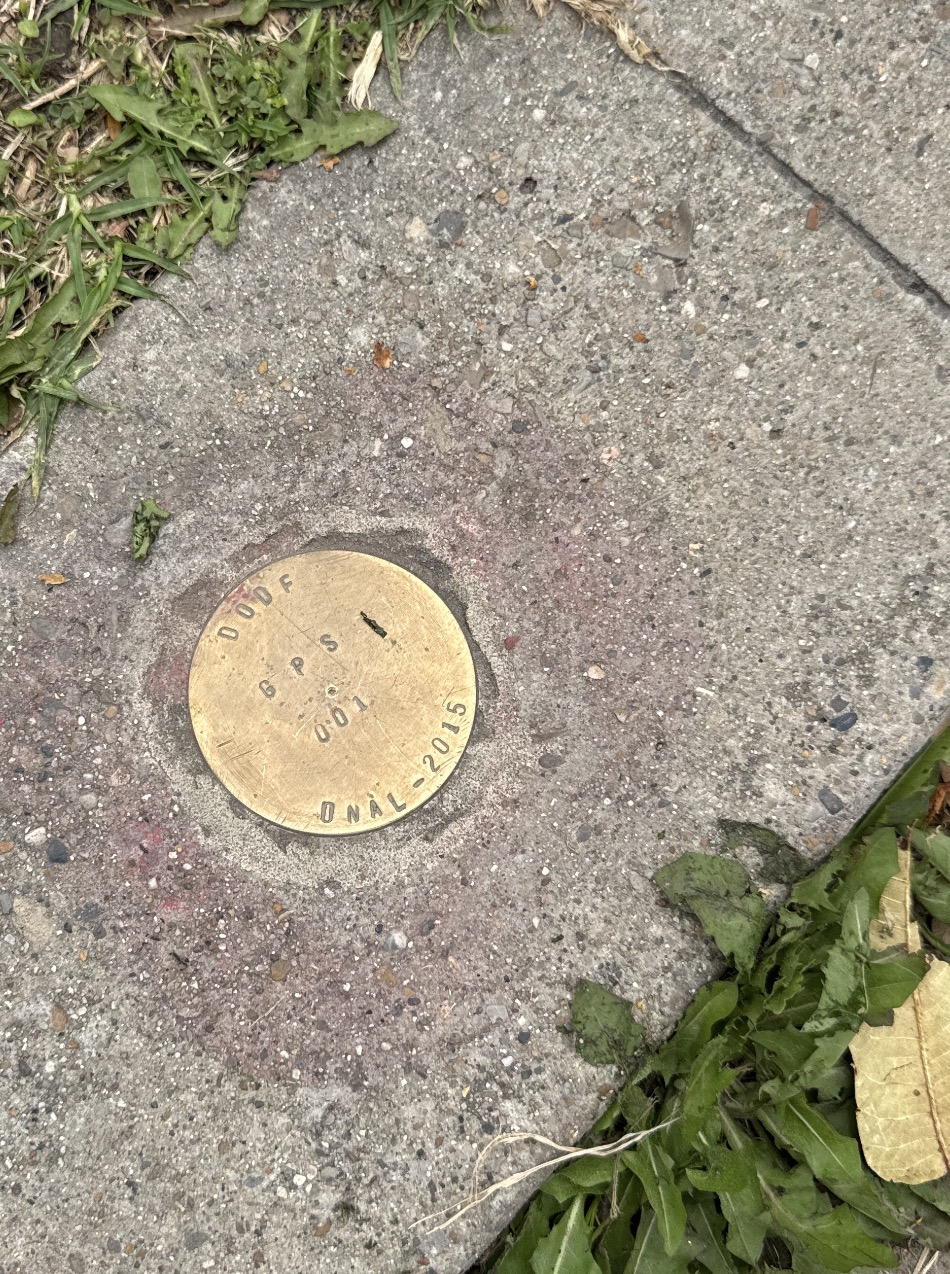
\includegraphics{53-practica_13_gnss_allynav_r26_files/img1.jpeg}

}

\subcaption{\label{fig-Vertice}Vértice DOOF UNAL}

\end{minipage}%
%
\begin{minipage}{0.50\linewidth}

\centering{

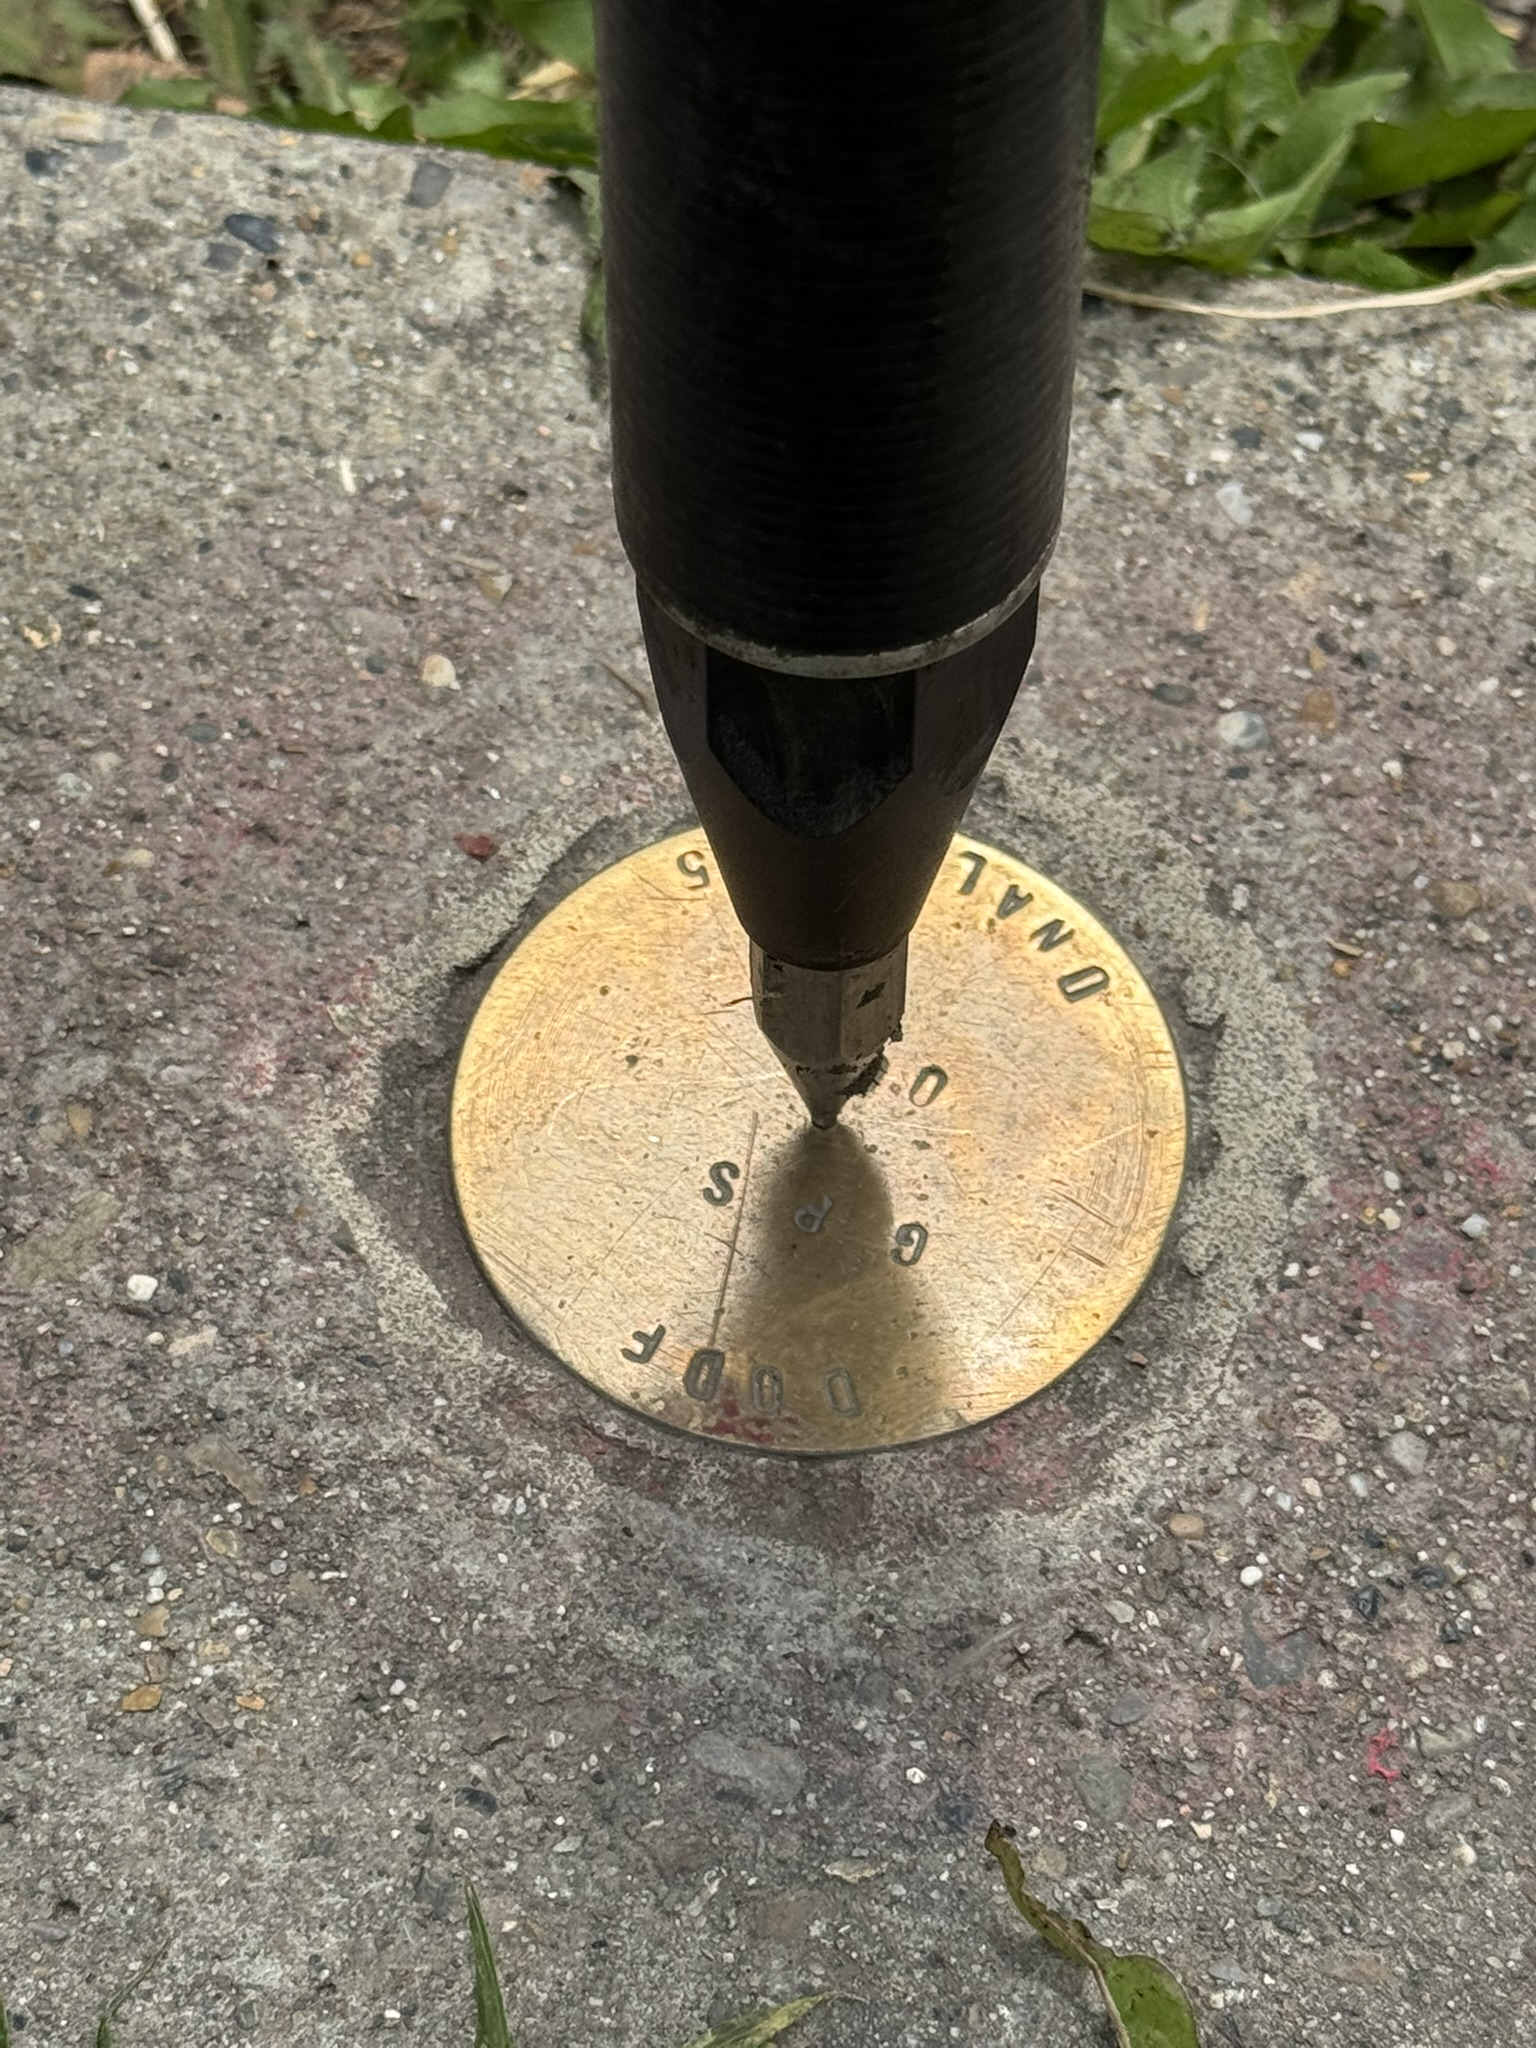
\includegraphics{53-practica_13_gnss_allynav_r26_files/img2.jpeg}

}

\subcaption{\label{fig-rover_V}Equipo AllyNav R26 en bastón (Rover)
sobre Vértice}

\end{minipage}%

\caption{\label{fig-vértice-unal}Fotos del vertice geodésico en el
campus de la Universidad Nacional.}

\end{figure}%

\begin{Shaded}
\begin{Highlighting}[]
\FunctionTok{library}\NormalTok{(leaflet)}

\CommentTok{\# Convertir coordenadas DMS a decimal para el mapa}
\CommentTok{\# 4°38\textquotesingle{}8.28" N {-}\textgreater{} 4.635633}
\CommentTok{\# 74°5\textquotesingle{}10.79" W {-}\textgreater{} {-}74.086331}

\FunctionTok{leaflet}\NormalTok{() }\SpecialCharTok{\%\textgreater{}\%}
  \FunctionTok{addTiles}\NormalTok{() }\SpecialCharTok{\%\textgreater{}\%}  \CommentTok{\# Añade el mapa base de OpenStreetMap}
  \FunctionTok{addMarkers}\NormalTok{(}\AttributeTok{lng =} \SpecialCharTok{{-}}\FloatTok{74.086331}\NormalTok{, }\AttributeTok{lat =} \FloatTok{4.635633}\NormalTok{, }
             \AttributeTok{popup =} \StringTok{"Vértice GPS{-}001 DODF\textless{}br\textgreater{}Universidad Nacional"}\NormalTok{) }\SpecialCharTok{\%\textgreater{}\%}
  \FunctionTok{setView}\NormalTok{(}\AttributeTok{lng =} \SpecialCharTok{{-}}\FloatTok{74.086331}\NormalTok{, }\AttributeTok{lat =} \FloatTok{4.635633}\NormalTok{, }\AttributeTok{zoom =} \DecValTok{16}\NormalTok{)}
\end{Highlighting}
\end{Shaded}

\begin{figure}[H]

\centering{

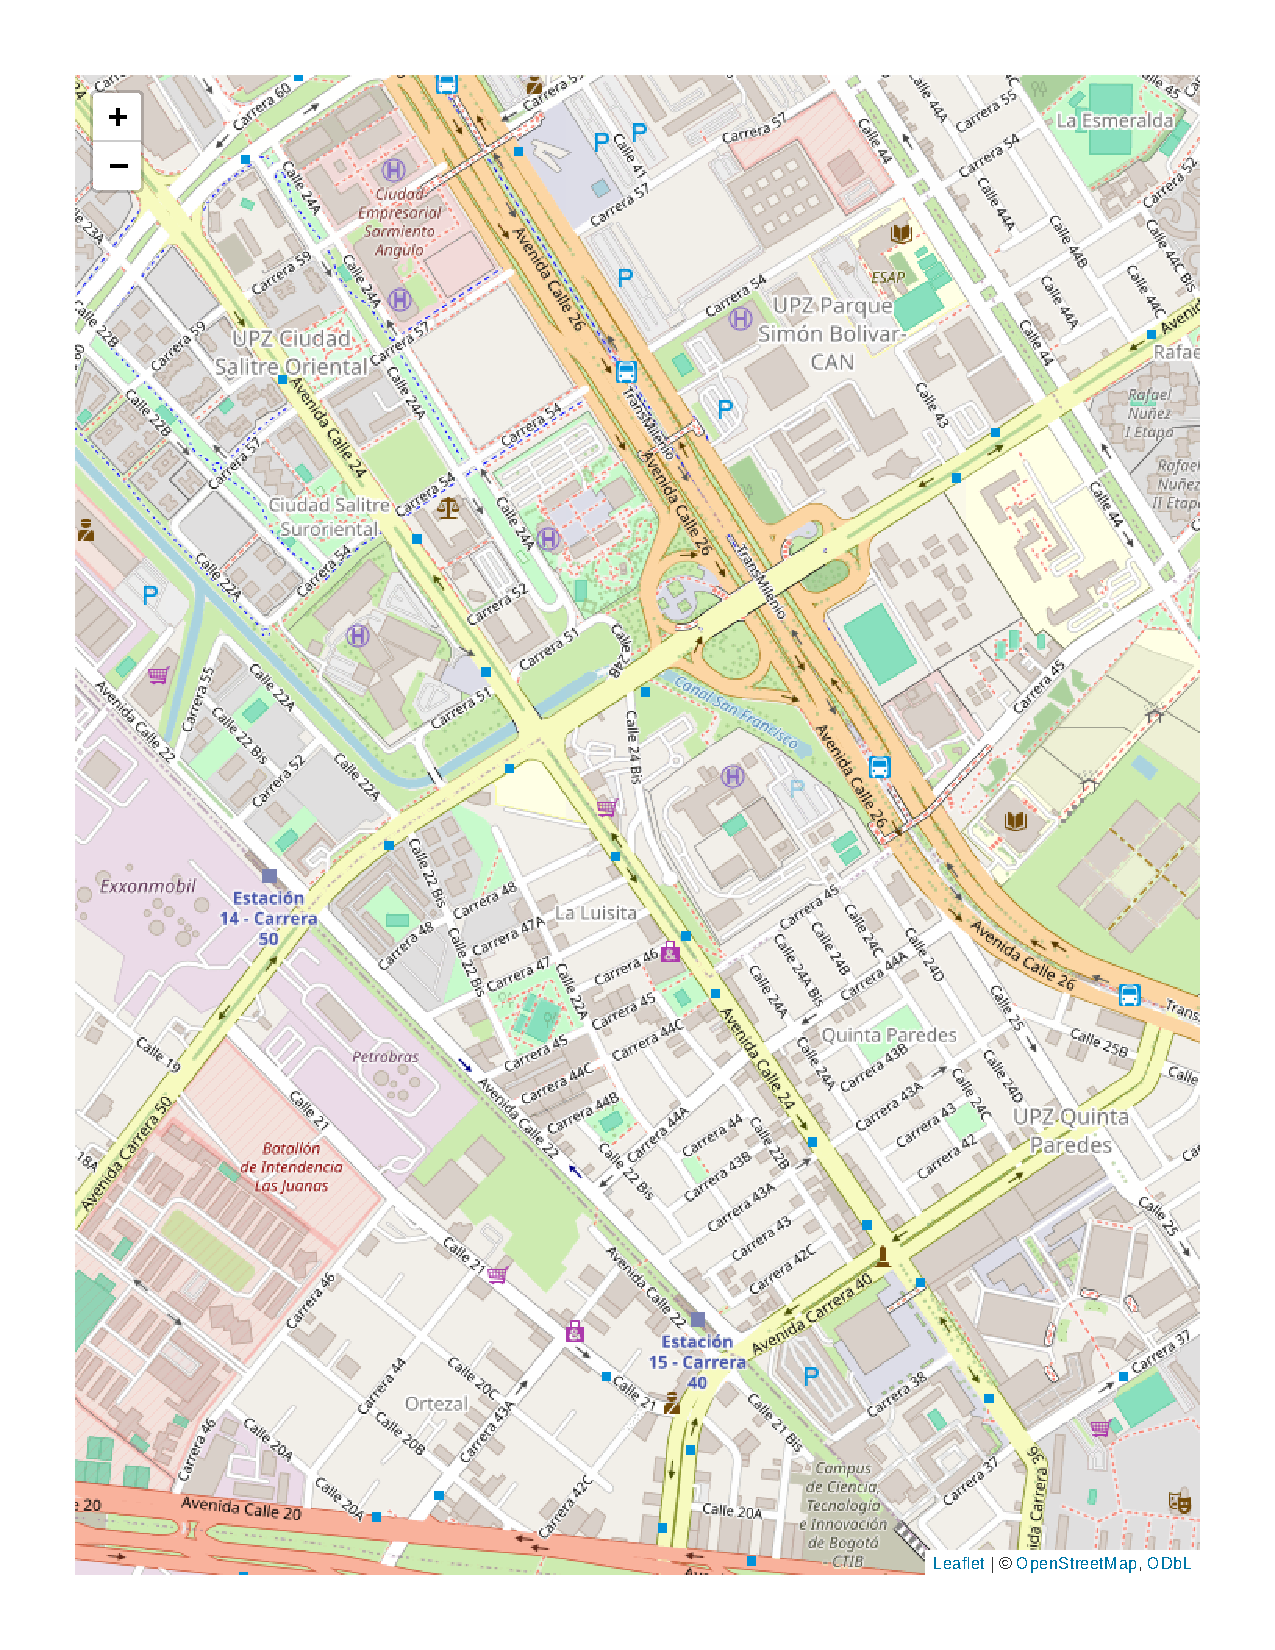
\includegraphics{53-practica_13_gnss_allynav_r26_files/figure-pdf/fig-mapa-geodesico-1.pdf}

}

\caption{\label{fig-mapa-geodesico}Ubicación del vértice geodésico
GPS-001 DODF (UNAL)}

\end{figure}%

El procedimiento incluye:

\begin{itemize}
\tightlist
\item
  Centrado y nivelación rigurosa sobre el vértice.
\item
  Medición y registro de la altura de antena, indicando el método
  empleado.
\item
  Configuración del receptor en modo estático para registrar
  observaciones GNSS crudas en formato binario.
\item
  Registro del nombre del punto, hora de inicio, hora final, condiciones
  de recepción y observaciones relevantes del entorno.
\item
  Tiempo mínimo de observación de 20 minutos para fines académicos y de
  comparación preliminar.
\end{itemize}

De acuerdo con la ficha técnica del AllyNav R26, la precisión nominal en
modo estático es de 2.5 mm + 1 ppm RMS en horizontal y 5 mm + 1 ppm RMS
en vertical. Sin embargo, dicha precisión depende del tiempo efectivo de
observación, la longitud de línea base, la geometría satelital, la
ausencia de obstrucciones, la correcta configuración de antena y la
calidad del postproceso. Por tanto, el tiempo de 20 minutos adoptado en
esta práctica debe entenderse como un criterio académico de observación
corta, y no como una garantía automática de exactitud geodésica final

\begin{tcolorbox}[enhanced jigsaw, colframe=quarto-callout-important-color-frame, bottomtitle=1mm, opacityback=0, toprule=.15mm, bottomrule=.15mm, left=2mm, breakable, rightrule=.15mm, opacitybacktitle=0.6, colback=white, toptitle=1mm, arc=.35mm, title=\textcolor{quarto-callout-important-color}{\faExclamation}\hspace{0.5em}{Important}, leftrule=.75mm, titlerule=0mm, coltitle=black, colbacktitle=quarto-callout-important-color!10!white]

\textbf{Nota sobre el tiempo de observación estática}

Para efectos de la presente práctica académica se adopta un tiempo
mínimo de observación de \textbf{20 minutos}, con el propósito de
registrar datos crudos y realizar una comparación preliminar entre la
solución estática y la solución RTK.

No obstante, para trabajos formales, el tiempo de rastreo debe definirse
en función de la distancia entre el punto observado y la base de
coordenadas conocidas, así como del tipo de equipo empleado. Como
referencia, el \textbf{IGAC} establece para levantamientos topográficos
de precisión la regla:

\[t = 15 + 5d\]

Donde: * \(t\): corresponde al tiempo de rastreo en minutos. * \(d\): es
la distancia en kilómetros a la base.

Para posicionamientos estáticos con equipos de doble frecuencia y
distancias menores a 80 km, se emplea también la expresión:

\[t = 65 + 3(d - 10)\]

En consecuencia, el tiempo de 20 minutos usado en esta práctica debe
entenderse como un criterio académico y no como un tiempo suficiente
para establecer control geodésico formal.

\end{tcolorbox}

Para esta práctica con el \textbf{AllyNav R26}, al ser un receptor
multiconstelación y multifrecuencia, la fórmula más coherente para un
posicionamiento estático formal sería:

\[t = 65 + 3(d - 10)\]

Pero si se trata de un levantamiento topográfico de precisión cercano a
la base, también es válido mencionar la regla:

\[t = 15 + 5d\]

\emph{Se recomienda documentar ambas, aclarando que corresponden a
escenarios de precisión y distancias distintas.}

\begin{quote}
Nota adicional: En el levantamiento estático, el receptor registra
observaciones GNSS crudas, por lo cual la definición del sistema de
referencia, proyección cartográfica, modelo geoidal y transformación de
coordenadas se realiza principalmente durante el postproceso. No
obstante, sí debe garantizarse el registro correcto del tipo de antena,
altura instrumental, método de medición de altura, nombre del punto y
tiempo efectivo de observación.
\end{quote}

\subsection{Levantamiento cinemático de borde de vía (Fase
RTK)}\label{levantamiento-cinemuxe1tico-de-borde-de-vuxeda-fase-rtk}

Concluida la fase estática, el receptor ubicado sobre el vértice
geodésico se configura como estación base RTK para transmitir
correcciones diferenciales mediante radio UHF. El segundo receptor se
configura como rover para recibir dichas correcciones en tiempo real y
realizar el levantamiento del borde de vía.

Esta configuración es distinta al modo de observación estática. En RTK,
la función principal de la base es ocupar un punto fijo de coordenadas
conocidas o previamente determinadas y transmitir correcciones
diferenciales al rover. De acuerdo con la ficha técnica del AllyNav R26,
la precisión nominal del método RTK es de 8 mm + 1 ppm RMS en horizontal
y 15 mm + 1 ppm RMS en vertical, bajo condiciones favorables de
recepción, adecuada comunicación base--rover y solución fija .

\begin{quote}
Nota: Para garantizar exactitud absoluta, la estación base debe
configurarse con las coordenadas oficiales del vértice o con coordenadas
obtenidas mediante postproceso. Si la base se inicializa con coordenadas
autónomas o promedio sin ajuste, los puntos levantados pueden conservar
buena precisión relativa entre sí, pero presentar desplazamientos
respecto al sistema oficial de referencia.
\end{quote}

\subsubsection{Procedimiento de levantamiento
cinemático:}\label{procedimiento-de-levantamiento-cinemuxe1tico}

\begin{itemize}
\tightlist
\item
  Se verifica la comunicación entre base y rover, el canal o frecuencia
  UHF, el formato de corrección diferencial y el tipo de solución
  obtenida.
\item
  Se aceptan preferiblemente puntos con solución fija ---Fixed---,
  comunicación estable y valores adecuados de precisión reportada.
\item
  El operador del rover se desplaza por el borde de la vía capturando
  vértices de manera rápida y dinámica, registrando observaciones
  relevantes en los puntos donde existan obstrucciones, pérdida de señal
  o dificultades de medición.
\item
  Se monitorean parámetros de calidad como número de satélites,
  geometría satelital, edad de corrección, HRMS, VRMS y estabilidad de
  la comunicación UHF.
\item
  Los puntos capturados con solución flotante ---Float---, pérdida de
  corrección, alta edad de corrección o valores elevados de HRMS/VRMS
  deberán repetirse o marcarse como observaciones de baja confiabilidad.
\item
  La compensación de inclinación se emplea únicamente cuando la IMU se
  encuentre correctamente inicializada y el ángulo de inclinación esté
  dentro del rango recomendado por el fabricante.
\end{itemize}

\section{Archivos de referencia y
resultados}\label{archivos-de-referencia-y-resultados}

Durante la práctica se generan y utilizan diferentes tipos de archivos,
dependiendo de la metodología de levantamiento empleada. En términos
generales, se cuenta con información asociada al levantamiento estático,
información correspondiente al levantamiento cinemático RTK y archivos
de referencia técnica y geodésica.

\subsection{Archivos del levantamiento
estático}\label{archivos-del-levantamiento-estuxe1tico}

Durante el levantamiento estático, el receptor AllyNav R26 instalado
sobre el punto geodésico registra internamente las observaciones GNSS
durante el tiempo de ocupación definido para la práctica. En este modo,
el equipo almacena en su memoria interna un archivo en formato TXT,
generado directamente por el receptor.

Este archivo contiene la información registrada durante la ocupación
estática, correspondiente a las observaciones y datos de navegación
capturados por el equipo mientras permaneció instalado sobre el vértice.
De acuerdo con la ficha técnica del AllyNav R26, el equipo permite
almacenar datos estáticos en formato binario y trabajar con información
GNSS para su posterior procesamiento .

Posteriormente, el archivo generado por el receptor se descarga al
computador y puede ser convertido a formato RINEX mediante diferentes
aplicaciones especializadas. En esta práctica se utiliza el software
NovAtel Convert, con el cual es posible transformar el archivo TXT
descargado del equipo en archivos RINEX.

El formato RINEX es ampliamente utilizado y aceptado por diferentes
programas de postproceso GNSS, por lo cual permite cargar las
observaciones en aplicaciones como RTKLIB, Leica Geo Office u otros
programas destinados al procesamiento diferencial o estático de
observaciones GNSS.

En síntesis, para la fase estática se tiene el siguiente flujo de
información:

\begin{longtable}[]{@{}
  >{\raggedright\arraybackslash}p{(\columnwidth - 4\tabcolsep) * \real{0.1298}}
  >{\raggedright\arraybackslash}p{(\columnwidth - 4\tabcolsep) * \real{0.2137}}
  >{\raggedright\arraybackslash}p{(\columnwidth - 4\tabcolsep) * \real{0.6565}}@{}}
\toprule\noalign{}
\begin{minipage}[b]{\linewidth}\raggedright
Etapa
\end{minipage} & \begin{minipage}[b]{\linewidth}\raggedright
Archivo o formato
\end{minipage} & \begin{minipage}[b]{\linewidth}\raggedright
Descripción
\end{minipage} \\
\midrule\noalign{}
\endhead
\bottomrule\noalign{}
\endlastfoot
Registro en campo & TXT generado por el receptor & Archivo almacenado en
la memoria interna del AllyNav R26 durante la ocupación estática \\
Descarga & TXT descargado al computador & Archivo original de
observaciones y navegación registrado por el equipo \\
Conversión & RINEX & Archivo convertido mediante NovAtel Convert para
ser usado en programas de postproceso \\
Postproceso & Resultados de coordenadas & Coordenadas ajustadas o
procesadas a partir de las observaciones estáticas \\
\end{longtable}

\subsection{Archivos del levantamiento cinemático
RTK}\label{archivos-del-levantamiento-cinemuxe1tico-rtk}

Para el levantamiento cinemático RTK, el receptor rover captura la
información de los puntos levantados mientras se encuentra enlazado a la
estación base mediante radios UHF. En esta configuración, la base
transmite correcciones diferenciales y el rover determina en tiempo real
las coordenadas de los puntos observados.

La captura, almacenamiento y administración de la información del
levantamiento RTK se realiza a través del colector de datos y de la
aplicación de campo utilizada con el equipo. Para esta práctica se
emplea la aplicación \emph{AllyPad}, desde la cual se crea el proyecto,
se configura el sistema de referencia, se definen los parámetros de
proyección y se almacenan los puntos capturados en campo.

Al momento de crear el proyecto en el colector, se debe definir
correctamente el datum, el elipsoide, el modelo de altura a emplear
---altura elipsoidal o geoide, si se dispone de uno--- y los parámetros
de proyección. Estos parámetros deben ser coherentes con las coordenadas
asignadas a la estación base al momento de configurarla. En esta
práctica, el colector se configuró para trabajar con el sistema
MAGNA-SIRGAS / Origen Nacional, también conocido como el origen único
nacional de Colombia.

Durante el levantamiento, la aplicación almacena información asociada a
cada punto capturado, incluyendo nombre o numeración del punto,
coordenadas, altura, descripción, hora de medición, precisión reportada
y referencia de la base desde la cual fue corregida la observación. Esta
información es importante porque permite identificar el origen de las
correcciones utilizadas, especialmente en casos donde la base se haya
instalado o configurado en más de un lugar durante una jornada de campo.

Una vez finalizado el levantamiento, los datos pueden exportarse desde
el colector mediante Bluetooth hacia un teléfono celular, computador u
otro dispositivo compatible. La información puede exportarse en
diferentes formatos, dependiendo de la configuración del proyecto y de
las necesidades del procesamiento posterior.

Los formatos más comunes son:

\textbf{Formatos de exportación y aplicaciones}

\begin{longtable}[]{@{}
  >{\raggedright\arraybackslash}p{(\columnwidth - 4\tabcolsep) * \real{0.3333}}
  >{\raggedright\arraybackslash}p{(\columnwidth - 4\tabcolsep) * \real{0.3333}}
  >{\raggedright\arraybackslash}p{(\columnwidth - 4\tabcolsep) * \real{0.3333}}@{}}
\caption{Formatos de salida y utilidad técnica de los datos
levantados}\label{tbl-formatos-salida}\tabularnewline
\toprule\noalign{}
\begin{minipage}[b]{\linewidth}\raggedright
Tipo de archivo
\end{minipage} & \begin{minipage}[b]{\linewidth}\raggedright
Contenido principal
\end{minipage} & \begin{minipage}[b]{\linewidth}\raggedright
Uso recomendado
\end{minipage} \\
\midrule\noalign{}
\endfirsthead
\toprule\noalign{}
\begin{minipage}[b]{\linewidth}\raggedright
Tipo de archivo
\end{minipage} & \begin{minipage}[b]{\linewidth}\raggedright
Contenido principal
\end{minipage} & \begin{minipage}[b]{\linewidth}\raggedright
Uso recomendado
\end{minipage} \\
\midrule\noalign{}
\endhead
\bottomrule\noalign{}
\endlastfoot
\textbf{CSV} & Nombre del punto, Este, Norte, altura y descripción & Uso
directo en hojas de cálculo, SIG (QGIS/ArcGIS) o CAD. \\
\textbf{TXT} & Coordenadas y atributos básicos de los puntos & Revisión
rápida, respaldo o importación a otros programas. \\
\textbf{Archivo bruto (Colector)} & Info completa: precisión, base,
fecha, hora y metadatos & Control de calidad y trazabilidad del
levantamiento RTK. \\
\textbf{Coordenadas Elipsoidales} & Latitud, longitud y altura
elipsoidal & Comparación geodésica o procesos de reproyección
posterior. \\
\textbf{Coordenadas Proyectadas} & Coordenada Este, Norte y altura & Uso
topográfico, cartográfico o aplicaciones de ingeniería. \\
\end{longtable}

\section{Archivos disponibles para la
práctica}\label{archivos-disponibles-para-la-pruxe1ctica}

Con base en la información recolectada en campo, para esta práctica se
cuenta principalmente con los siguientes archivos:

\subsection{Inventario de archivos y documentación de la
práctica}\label{inventario-de-archivos-y-documentaciuxf3n-de-la-pruxe1ctica}

\begin{longtable}[]{@{}
  >{\raggedright\arraybackslash}p{(\columnwidth - 2\tabcolsep) * \real{0.2927}}
  >{\raggedright\arraybackslash}p{(\columnwidth - 2\tabcolsep) * \real{0.7073}}@{}}
\caption{Organización de la información y archivos de
respaldo}\label{tbl-anexos}\tabularnewline
\toprule\noalign{}
\begin{minipage}[b]{\linewidth}\raggedright
Archivo o directorio
\end{minipage} & \begin{minipage}[b]{\linewidth}\raggedright
Descripción
\end{minipage} \\
\midrule\noalign{}
\endfirsthead
\toprule\noalign{}
\begin{minipage}[b]{\linewidth}\raggedright
Archivo o directorio
\end{minipage} & \begin{minipage}[b]{\linewidth}\raggedright
Descripción
\end{minipage} \\
\midrule\noalign{}
\endhead
\bottomrule\noalign{}
\endlastfoot
\texttt{R26-Datasheet.pdf} & Ficha técnica del receptor AllyNav R26:
modos base/rover, radio UHF y precisiones nominales. \\
\texttt{red\_geodesica\_unal.txt} & Coordenadas oficiales del punto de
referencia (IGAC/UNAL). \\
\texttt{Datos\ de\ Levantamiento\ Estático.txt} & Datos crudos de la
ocupación sobre el punto geodésico. \\
\texttt{RINEX/} (Carpeta) & Archivos de observación y navegación
convertidos para postproceso. \\
\texttt{Crudos/} (Carpeta) & Archivos originales (binarios) descargados
directamente del equipo. \\
\texttt{UNAL3\_103121.xls} & Archivo de resultados o exportación del
levantamiento de campo. \\
\texttt{UNALclase\_102348.txt} & Archivo de exportación del
levantamiento realizado en la práctica. \\
\texttt{UNAL\_102813.txt} & Archivo de exportación adicional de los
puntos levantados. \\
\texttt{GNSS\ Clase.rar} & Paquete comprimido con el backup completo
(Crudos, RINEX y Estático). \\
\end{longtable}

En el documento original ya se relacionan estos archivos como parte de
los insumos de la práctica, incluyendo el datasheet del equipo, las
coordenadas de referencia, los archivos TXT, XLS, el archivo comprimido
y las carpetas de datos crudos y RINEX

\subsection{Consideraciones sobre los formatos de
salida}\label{consideraciones-sobre-los-formatos-de-salida}

Es importante diferenciar los archivos generados en la fase estática de
los generados en la fase RTK. En el levantamiento estático, el archivo
principal corresponde al registro de observaciones del receptor, el cual
posteriormente se convierte a RINEX para ser procesado. En cambio, en el
levantamiento RTK, la información principal corresponde a las
coordenadas de los puntos capturados en tiempo real por el rover y
almacenadas en el colector de datos mediante la aplicación AllyPad.

Por tanto, para esta práctica se cuenta, en general, con dos grupos de
información:

\subsection{Síntesis de los métodos de levantamiento
realizados}\label{suxedntesis-de-los-muxe9todos-de-levantamiento-realizados}

\begin{longtable}[]{@{}
  >{\raggedright\arraybackslash}p{(\columnwidth - 4\tabcolsep) * \real{0.2400}}
  >{\raggedright\arraybackslash}p{(\columnwidth - 4\tabcolsep) * \real{0.2000}}
  >{\raggedright\arraybackslash}p{(\columnwidth - 4\tabcolsep) * \real{0.5600}}@{}}
\caption{Clasificación de datos según el método de
observación}\label{tbl-metodologia-resumen}\tabularnewline
\toprule\noalign{}
\begin{minipage}[b]{\linewidth}\raggedright
Grupo de información
\end{minipage} & \begin{minipage}[b]{\linewidth}\raggedright
Archivo principal
\end{minipage} & \begin{minipage}[b]{\linewidth}\raggedright
Propósito
\end{minipage} \\
\midrule\noalign{}
\endfirsthead
\toprule\noalign{}
\begin{minipage}[b]{\linewidth}\raggedright
Grupo de información
\end{minipage} & \begin{minipage}[b]{\linewidth}\raggedright
Archivo principal
\end{minipage} & \begin{minipage}[b]{\linewidth}\raggedright
Propósito
\end{minipage} \\
\midrule\noalign{}
\endhead
\bottomrule\noalign{}
\endlastfoot
\textbf{Levantamiento estático} & \texttt{.TXT} del receptor (convertido
a \textbf{RINEX}) & Postproceso GNSS y comparación con coordenadas
oficiales del vértice. \\
\textbf{Levantamiento RTK} & \texttt{.CSV}, \texttt{.TXT} o formato
bruto (AllyPad) & Obtención de coordenadas precisas de los puntos de
detalle en campo. \\
\end{longtable}

Los archivos exportados desde AllyPad pueden contener coordenadas
elipsoidales ---latitud, longitud y altura elipsoidal--- o coordenadas
proyectadas ---Este, Norte y altura---, dependiendo de la configuración
definida en el proyecto. Para esta práctica, cuando se requiera trabajar
directamente en un sistema plano de coordenadas, se emplea la
configuración correspondiente a MAGNA-SIRGAS / Origen Nacional.

La información recolectada durante la práctica, incluyendo los archivos
asociados al levantamiento estático, los archivos convertidos a formato
RINEX, los datos crudos descargados del receptor y las exportaciones
correspondientes al levantamiento cinemático RTK, se encuentra
disponible en el siguiente enlace: La información se encuentra en la
ruta local:

\texttt{C:\textbackslash{}Guia\_practica\_GNSS\textbackslash{}53-practica\_13\_gnss\_allynav\_r26\_files\textbackslash{}Info-campo}

\section{Postproceso de información de campo (Trabajo de
oficina)}\label{postproceso-de-informaciuxf3n-de-campo-trabajo-de-oficina}

Como fase complementaria al trabajo de campo, se plantea una sesión de
escritorio dedicada al postproceso de la información. El objetivo es que
los estudiantes comprendan cómo se obtienen coordenadas ajustadas a
partir de los datos brutos observados, analizando la diferencia entre
una solución obtenida en tiempo real (RTK) y una solución derivada del
procesamiento de oficina.

Una vez revisada y organizada la información recolectada en campo, el
postproceso se desarrolla en dos etapas principales: primero, el
procesamiento del \textbf{levantamiento estático} realizado sobre la
base; y posteriormente, la revisión o corrección del
\textbf{levantamiento cinemático RTK}, el cual depende de la coordenada
ajustada de dicha base.

En esta práctica, el levantamiento RTK del borde de vía fue realizado
tomando como referencia la estación base instalada sobre el vértice
geodésico. Por esta razón, antes de validar o ajustar las coordenadas de
los puntos levantados con el rover, es necesario procesar la observación
estática de la base, obtener una coordenada corregida y comparar dicha
coordenada con la utilizada inicialmente durante el levantamiento en
campo.

La finalidad de este procedimiento es determinar si existe un
desplazamiento entre la coordenada inicialmente asignada a la base
durante el levantamiento RTK y la coordenada obtenida mediante
postproceso. En caso de existir dicho desplazamiento, las coordenadas
del levantamiento cinemático podrán corregirse trasladándolas en función
de la diferencia encontrada.

\begin{figure}[H]

{\centering 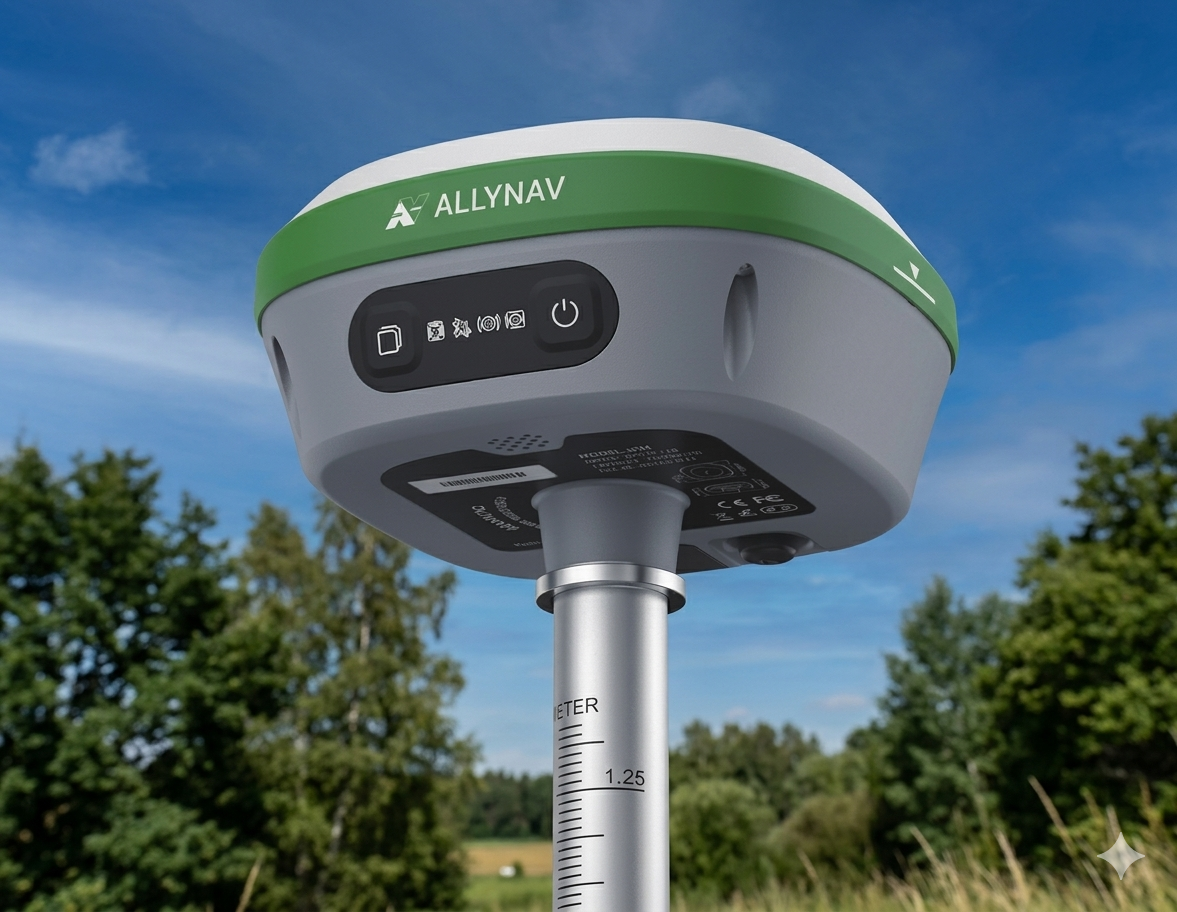
\includegraphics{./53-practica_13_gnss_allynav_r26_files/Img0.png}

}

\caption{Receptor AllyNav R26 utilizado en la práctica}

\end{figure}%

\subsection{Organización inicial de la
información}\label{organizaciuxf3n-inicial-de-la-informaciuxf3n}

El primer paso consiste en organizar los archivos recolectados en campo,
separando la información correspondiente al levantamiento estático y la
información asociada al levantamiento cinemático RTK.

Para esta práctica se cuenta, en general, con dos grupos principales de
archivos:

\begin{longtable}[]{@{}
  >{\raggedright\arraybackslash}p{(\columnwidth - 4\tabcolsep) * \real{0.3333}}
  >{\raggedright\arraybackslash}p{(\columnwidth - 4\tabcolsep) * \real{0.3333}}
  >{\raggedright\arraybackslash}p{(\columnwidth - 4\tabcolsep) * \real{0.3333}}@{}}
\toprule\noalign{}
\begin{minipage}[b]{\linewidth}\raggedright
Grupo de información
\end{minipage} & \begin{minipage}[b]{\linewidth}\raggedright
Archivo principal
\end{minipage} & \begin{minipage}[b]{\linewidth}\raggedright
Propósito
\end{minipage} \\
\midrule\noalign{}
\endhead
\bottomrule\noalign{}
\endlastfoot
Levantamiento estático & Archivo TXT generado por el receptor &
Conversión a RINEX y postproceso de la base \\
Levantamiento cinemático RTK & Archivos exportados desde AllyPad &
Revisión o corrección de las coordenadas levantadas con el rover \\
\end{longtable}

Durante el levantamiento estático, el equipo instalado sobre el punto
geodésico registra internamente un archivo en formato \textbf{TXT}, el
cual contiene las observaciones y datos de navegación capturados durante
el tiempo de rastreo. Este archivo debe descargarse desde la memoria
interna del receptor para su posterior conversión y procesamiento.

En el levantamiento cinemático RTK, la información se almacena en el
colector de datos mediante la aplicación \textbf{AllyPad}. Allí se
guardan las coordenadas de los puntos levantados, la numeración o nombre
del punto, la descripción, la altura, la precisión reportada, la fecha y
hora de captura, así como la información de la base desde la cual se
recibieron las correcciones.

\subsection{Información de campo
requerida}\label{informaciuxf3n-de-campo-requerida}

Antes de iniciar el postproceso, se debe verificar que la bitácora de
campo contenga la información mínima necesaria para configurar
correctamente el procesamiento.

Durante la ocupación estática se debe haber registrado:

\begin{longtable}[]{@{}
  >{\raggedright\arraybackslash}p{(\columnwidth - 2\tabcolsep) * \real{0.5000}}
  >{\raggedright\arraybackslash}p{(\columnwidth - 2\tabcolsep) * \real{0.5000}}@{}}
\toprule\noalign{}
\begin{minipage}[b]{\linewidth}\raggedright
Información
\end{minipage} & \begin{minipage}[b]{\linewidth}\raggedright
Descripción
\end{minipage} \\
\midrule\noalign{}
\endhead
\bottomrule\noalign{}
\endlastfoot
Nombre del punto & Identificación del vértice observado \\
Hora de inicio & Hora en la que comenzó el rastreo estático \\
Hora de finalización & Hora en la que terminó el rastreo \\
Altura de antena & Distancia medida entre la marca de referencia de la
antena y el punto físico ocupado \\
Tipo de altura & Indicar si la altura fue medida de forma vertical o
inclinada \\
Localización del punto & Descripción de la ubicación de la placa o
vértice \\
Condiciones del entorno & Obstáculos, árboles, edificaciones u otros
elementos que puedan afectar la señal \\
Condiciones atmosféricas & Estado general del clima durante la
observación \\
Esquema de localización & Croquis o descripción gráfica del punto
observado \\
\end{longtable}

La correcta medición de la altura de antena es fundamental, ya que un
error en este dato se refleja directamente en la altura final obtenida
durante el postproceso.

\begin{figure}[H]

{\centering 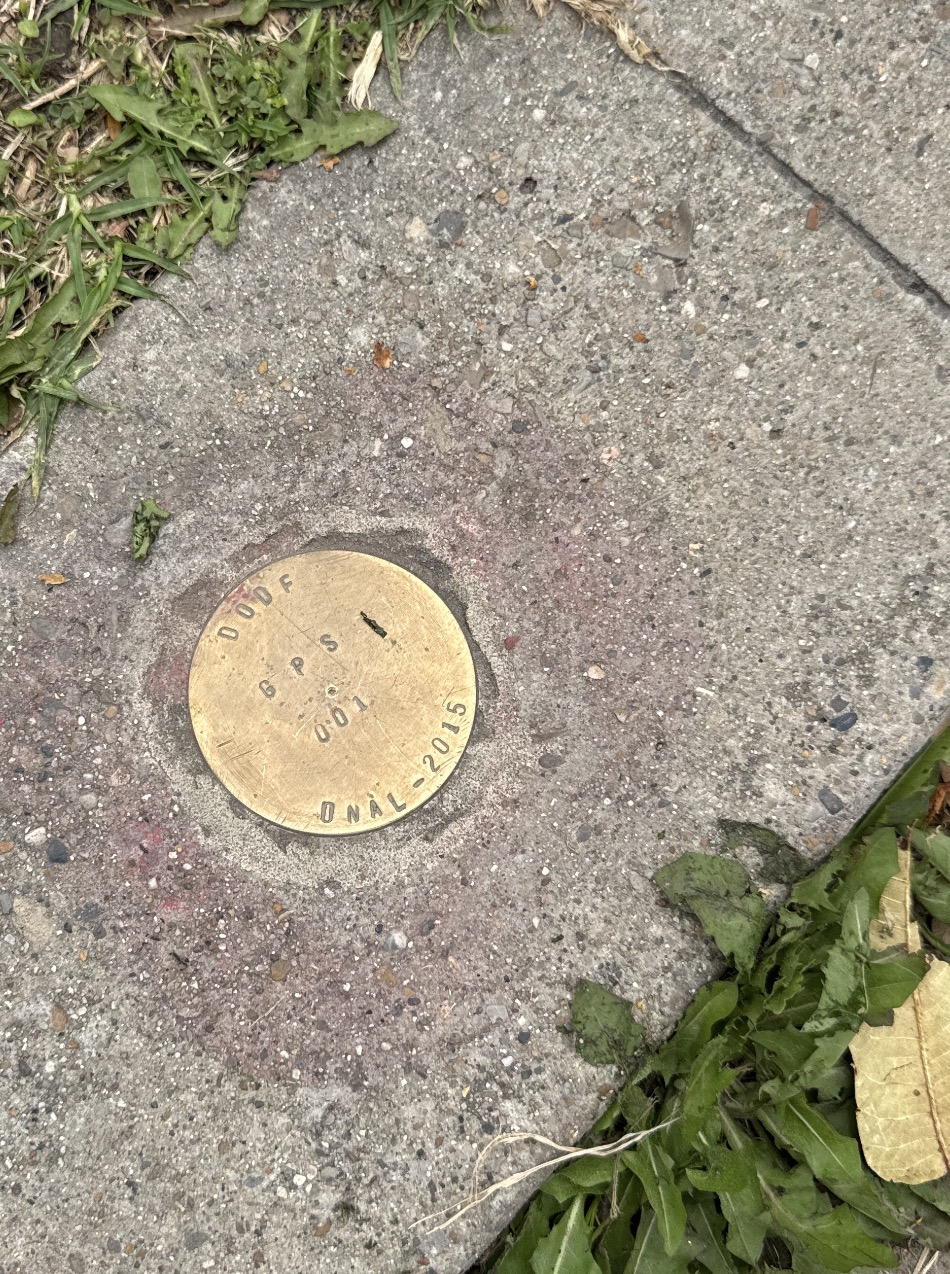
\includegraphics{./53-practica_13_gnss_allynav_r26_files/img1.jpeg}

}

\caption{Placa del vértice geodésico utilizado para la ocupación
estática}

\end{figure}%

\subsection{Conversión del archivo TXT a formato
RINEX}\label{conversiuxf3n-del-archivo-txt-a-formato-rinex}

Una vez descargado el archivo TXT generado por el receptor durante el
rastreo estático, se debe convertir a un formato compatible con
aplicaciones de postproceso GNSS. Para esta práctica se utiliza la
aplicación \textbf{NovAtel Convert}, disponible en el siguiente enlace:

\url{https://novatel.com/support/support-materials/software-downloads}

El procedimiento general consiste en abrir el archivo TXT desde la
aplicación, seleccionar el formato de salida requerido y ejecutar la
conversión mediante el botón \textbf{Convert}. El archivo puede
exportarse, por ejemplo, en formato \textbf{RINEX 2.11} o \textbf{RINEX
3.1}, según los requerimientos del software de postproceso que se vaya a
utilizar.

Como resultado de la conversión se generan archivos RINEX asociados a
las observaciones y a la navegación satelital. Estos archivos quedan
almacenados normalmente en la misma carpeta donde se encuentra el
archivo TXT original.

\begin{longtable}[]{@{}ll@{}}
\toprule\noalign{}
Extensión & Contenido \\
\midrule\noalign{}
\endhead
\bottomrule\noalign{}
\endlastfoot
\texttt{.O} & Archivo de observaciones GNSS \\
\texttt{.N} o \texttt{.D} & Archivo de navegación satelital \\
\texttt{.G} & Archivo de navegación GLONASS, cuando aplica \\
\end{longtable}

Estos archivos constituyen la información básica del punto observado y
serán utilizados posteriormente en el software de postproceso.

\begin{figure}[H]

{\centering 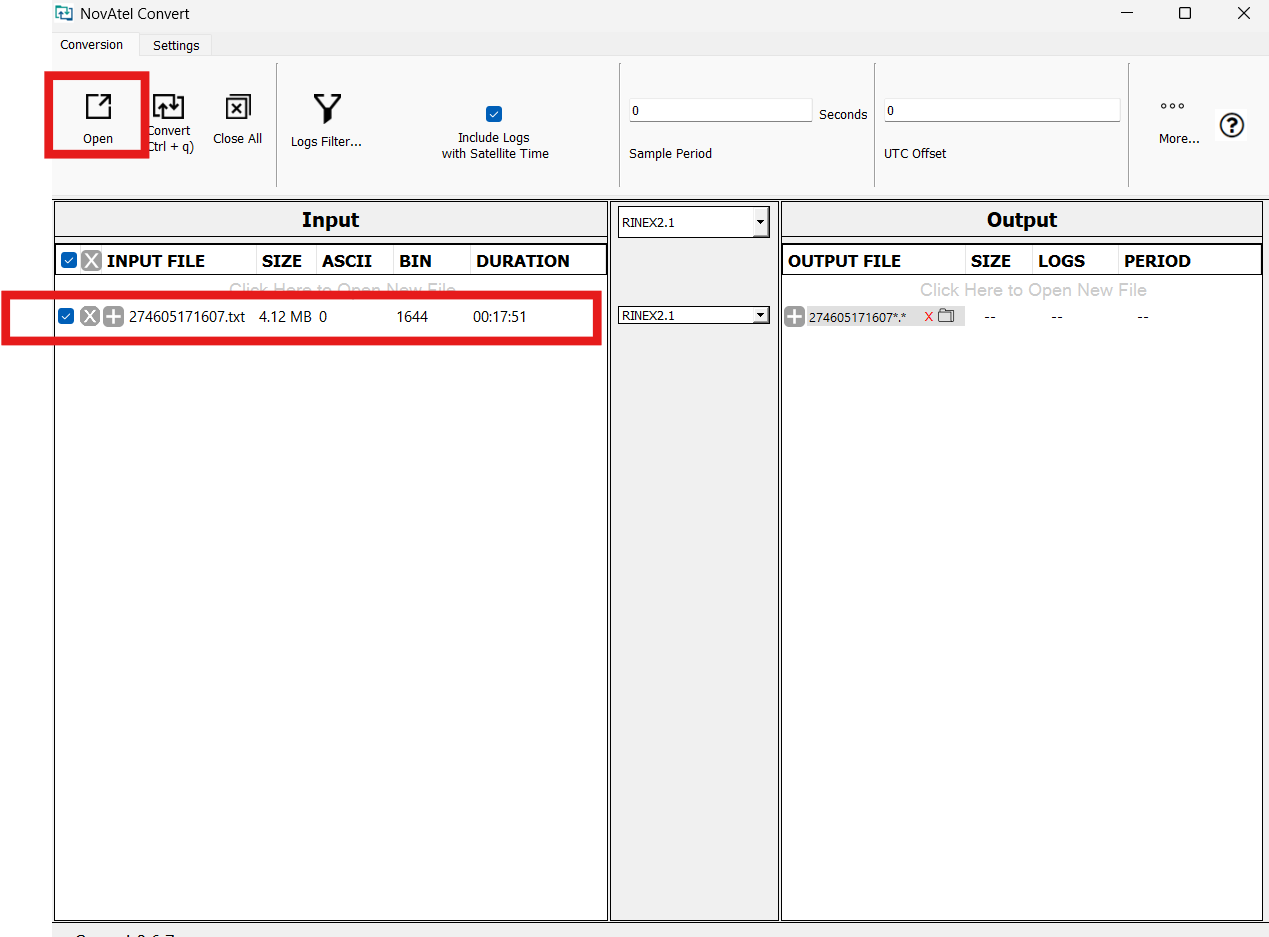
\includegraphics{./53-practica_13_gnss_allynav_r26_files/convert_txt_rinex.png}

}

\caption{Conversión del archivo TXT del receptor a formato RINEX
mediante NovAtel Convert}

\end{figure}%%
\begin{figure}[H]

{\centering 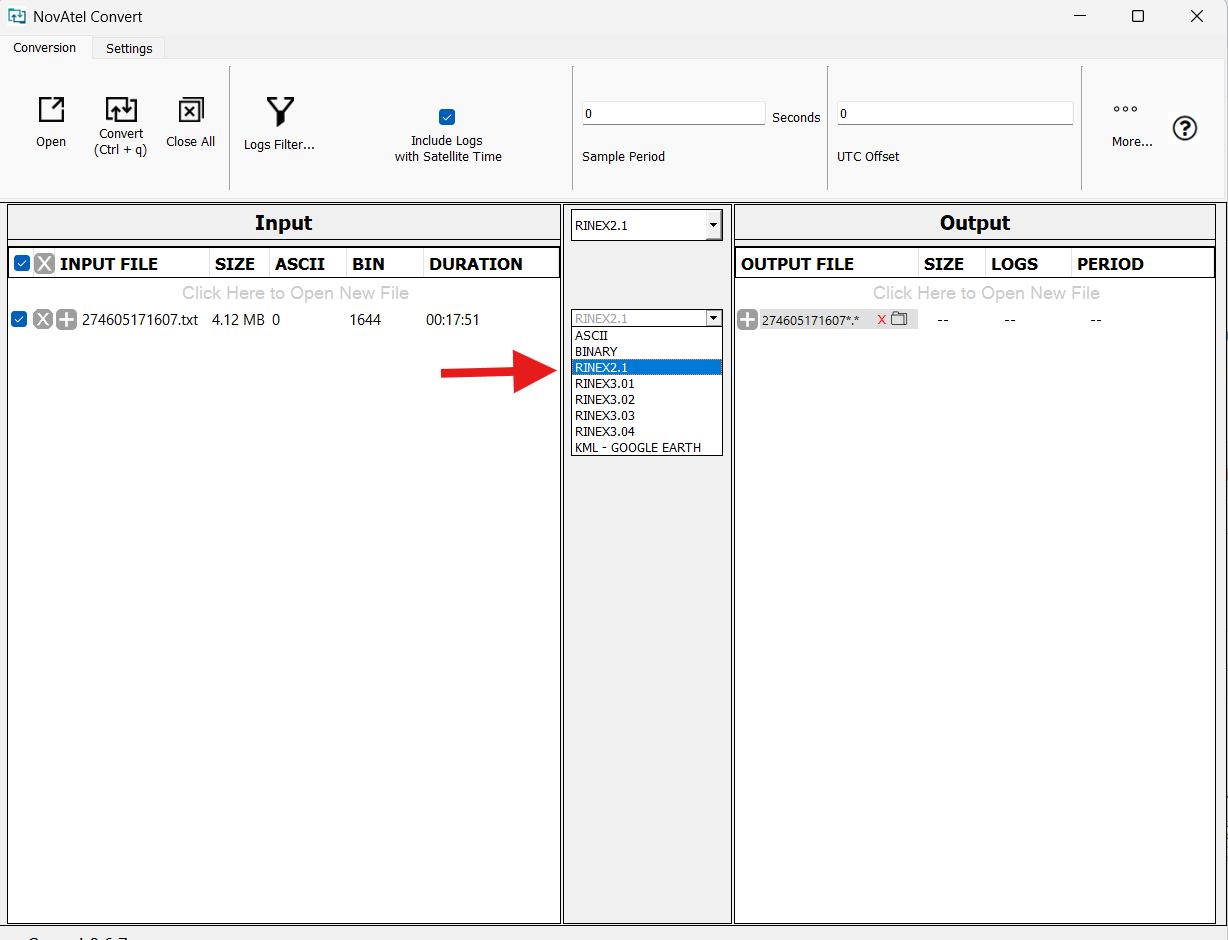
\includegraphics{./53-practica_13_gnss_allynav_r26_files/formato_rinex.png}

}

\caption{Selección del formato de salida RINEX 2.11 o RINEX 3.1}

\end{figure}%%
\begin{figure}[H]

{\centering 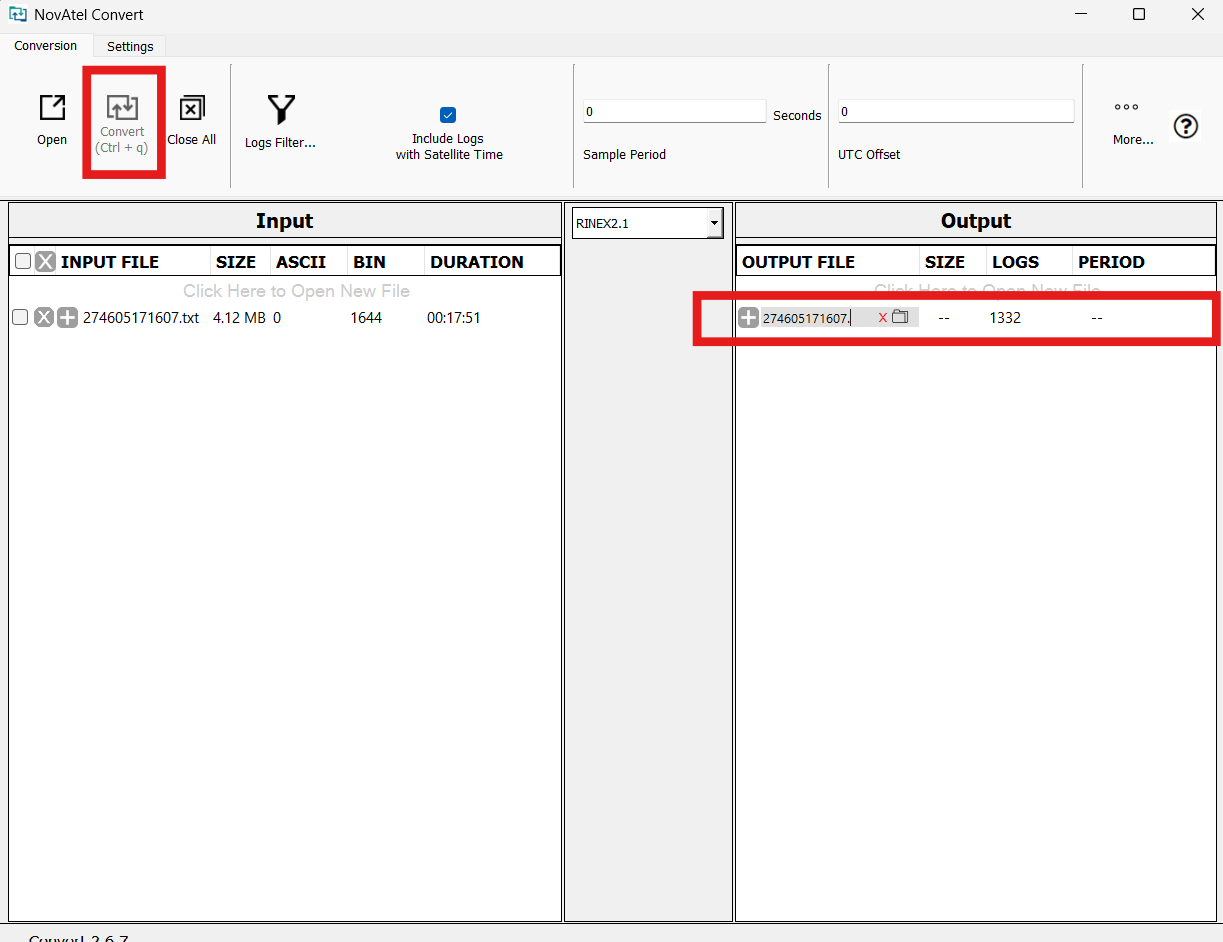
\includegraphics{./53-practica_13_gnss_allynav_r26_files/formato_rinexconv.png}

}

\caption{Conversión RINEX 2.11 o RINEX 3.1}

\end{figure}%%
\begin{figure}[H]

{\centering 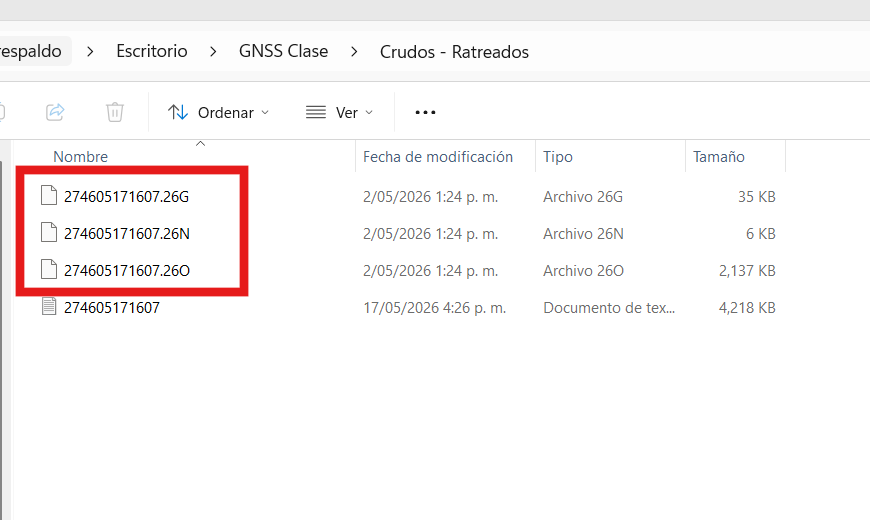
\includegraphics{./53-practica_13_gnss_allynav_r26_files/rinex_generados.png}

}

\caption{Archivos RINEX generados a partir del rastreo estático}

\end{figure}%

\subsection{Descarga de archivos RINEX de una estación permanente del
IGAC}\label{descarga-de-archivos-rinex-de-una-estaciuxf3n-permanente-del-igac}

Una vez obtenidos los archivos RINEX del punto observado, se deben
descargar los archivos RINEX de una estación permanente de referencia
perteneciente a la Red Activa GNSS del IGAC.

Para ello se ingresa al geoportal geodésico del IGAC:

\url{https://redgeodesica.igac.gov.co/red_activa.html}

Desde la Red Activa GNSS se identifica la estación permanente más
cercana al punto observado. Para facilitar esta selección, puede
emplearse el visor geográfico de la Red Geodésica Nacional, donde se
visualizan las estaciones disponibles, su localización, nombre y estado
de operación.

Posteriormente, se busca la estación por nombre y se descargan los
archivos RINEX correspondientes a la misma fecha del levantamiento. La
búsqueda puede realizarse por nombre de estación, fecha calendario,
semana GNSS o día del año.

\begin{figure}[H]

{\centering 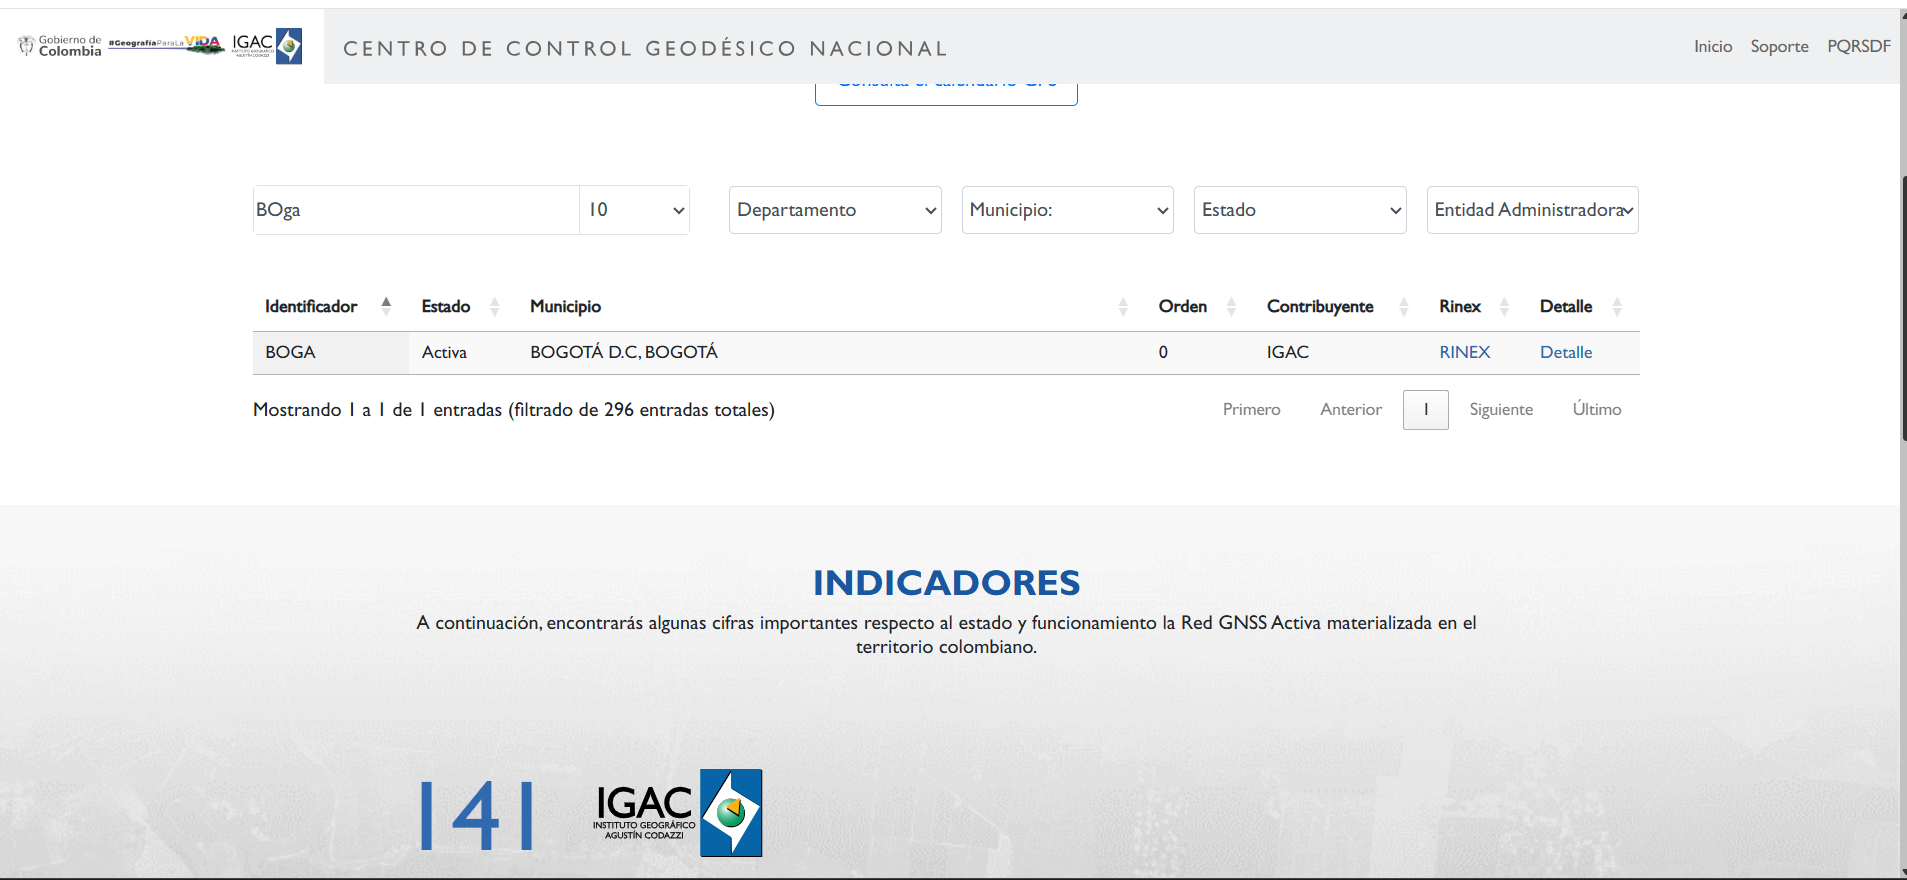
\includegraphics{./53-practica_13_gnss_allynav_r26_files/BOGA1.png}

}

\caption{Consulta de la Red Activa GNSS del IGAC}

\end{figure}%%
\begin{figure}[H]

{\centering 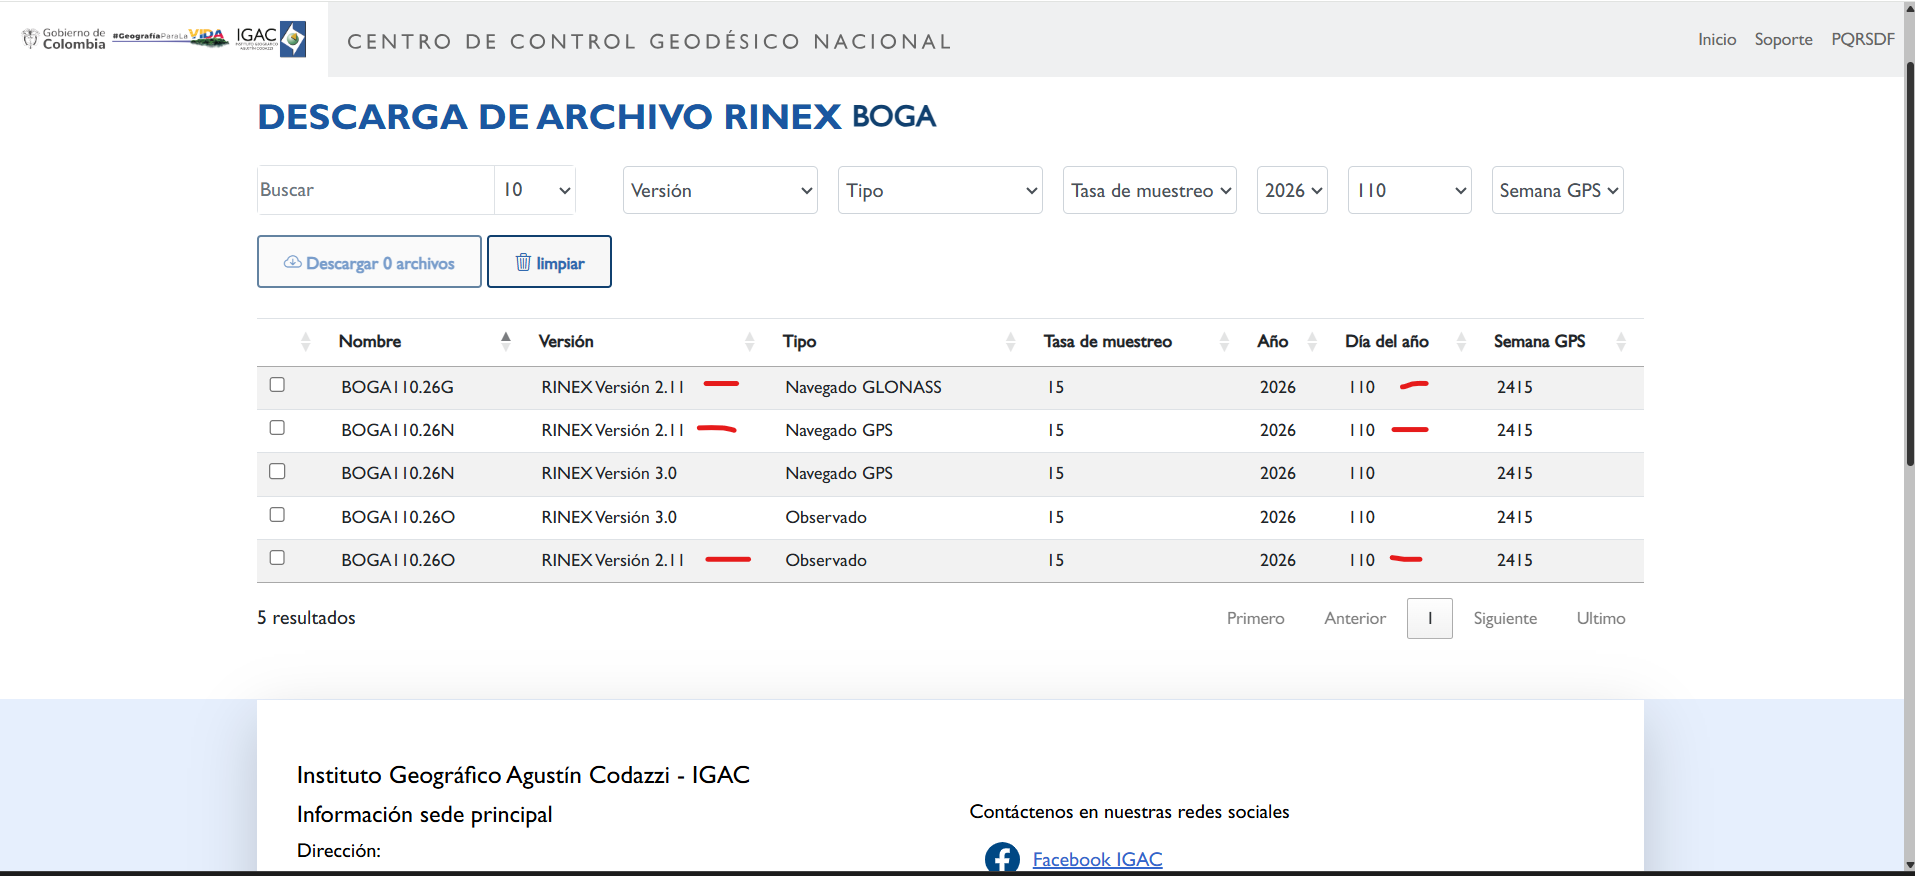
\includegraphics{./53-practica_13_gnss_allynav_r26_files/BOGA2.png}

}

\caption{Selección y descarga de archivos RINEX de la estación BOGA}

\end{figure}%

Para esta práctica se emplea la estación \textbf{BOGA}, localizada
dentro del campus de la Universidad Nacional de Colombia y disponible
como estación activa. De esta estación se descargan los archivos RINEX
correspondientes al día del levantamiento, en formato \textbf{RINEX
2.11}.

Los archivos descargados de la estación permanente se utilizarán como
referencia para procesar diferencialmente el punto observado durante la
ocupación estática.

\subsection{Descarga de efemérides
precisas}\label{descarga-de-efemuxe9rides-precisas}

Adicionalmente, se descargan las \textbf{efemérides precisas}
correspondientes a la semana GNSS y al día específico del levantamiento.
Estas efemérides permiten mejorar la calidad del procesamiento, al
utilizar información orbital más precisa que la contenida en los
archivos de navegación transmitidos por los satélites.

En esta práctica, el levantamiento fue realizado en la \textbf{semana
GPS 2415}, día \textbf{110}, por lo cual deben descargarse las
efemérides precisas correspondientes a dicha semana y fecha.

Por medio de la siguiente página podemos confirmar el numero de la
semana GNSS y el dia Calendario que corresponde:
https://gnsscalendar.com/

\begin{figure}[H]

{\centering 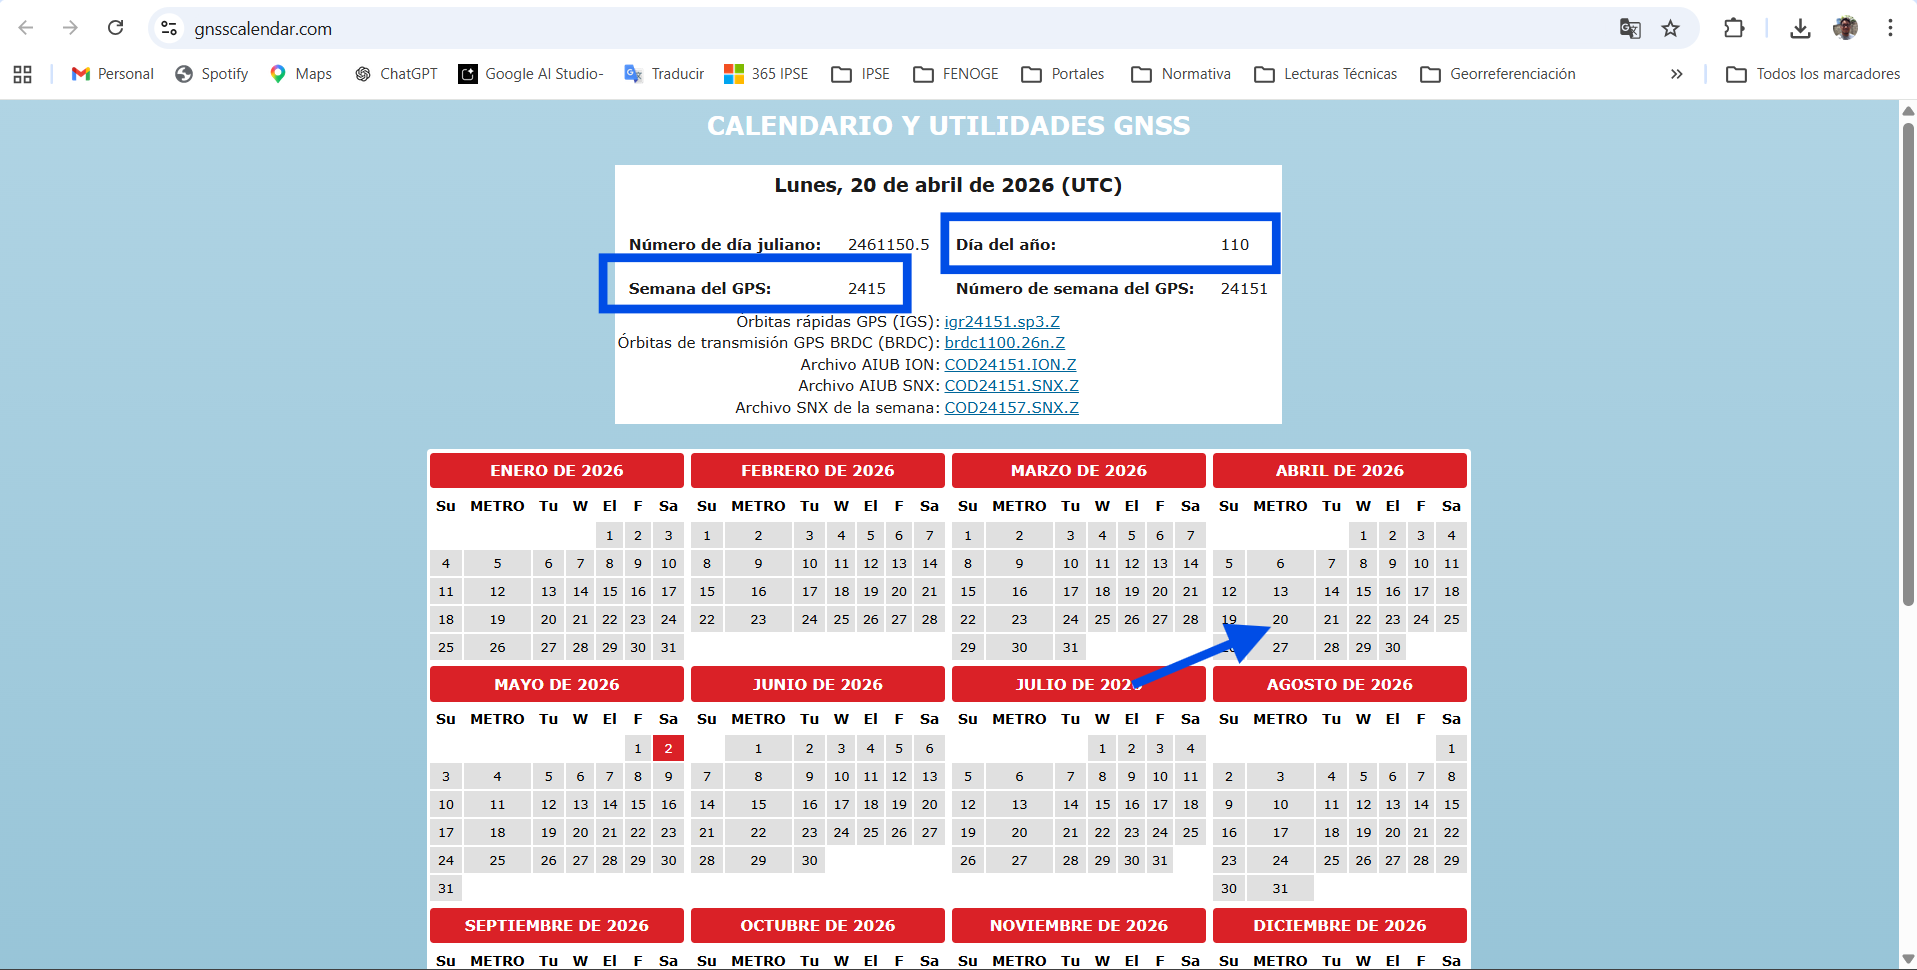
\includegraphics{./53-practica_13_gnss_allynav_r26_files/semana_gps.png}

}

\caption{Selección de semana GNSS y día correspondiente al
levantamiento}

\end{figure}%

Estas efemérides serán utilizadas en el procesamiento cuando el software
lo permita. En particular, se realizará una comparación entre el
procesamiento efectuado con una aplicación de libre acceso que no
permite incorporar efemérides precisas y el procesamiento realizado con
\textbf{RTKLIB}, específicamente mediante el módulo \textbf{RTKPOST},
donde sí es posible cargarlas.

Acceso a pagina de descarga de Efemérides:
https://www.earthdata.nasa.gov/data/space-geodesy-techniques/gnss/precise-orbits-product

\begin{figure}[H]

{\centering 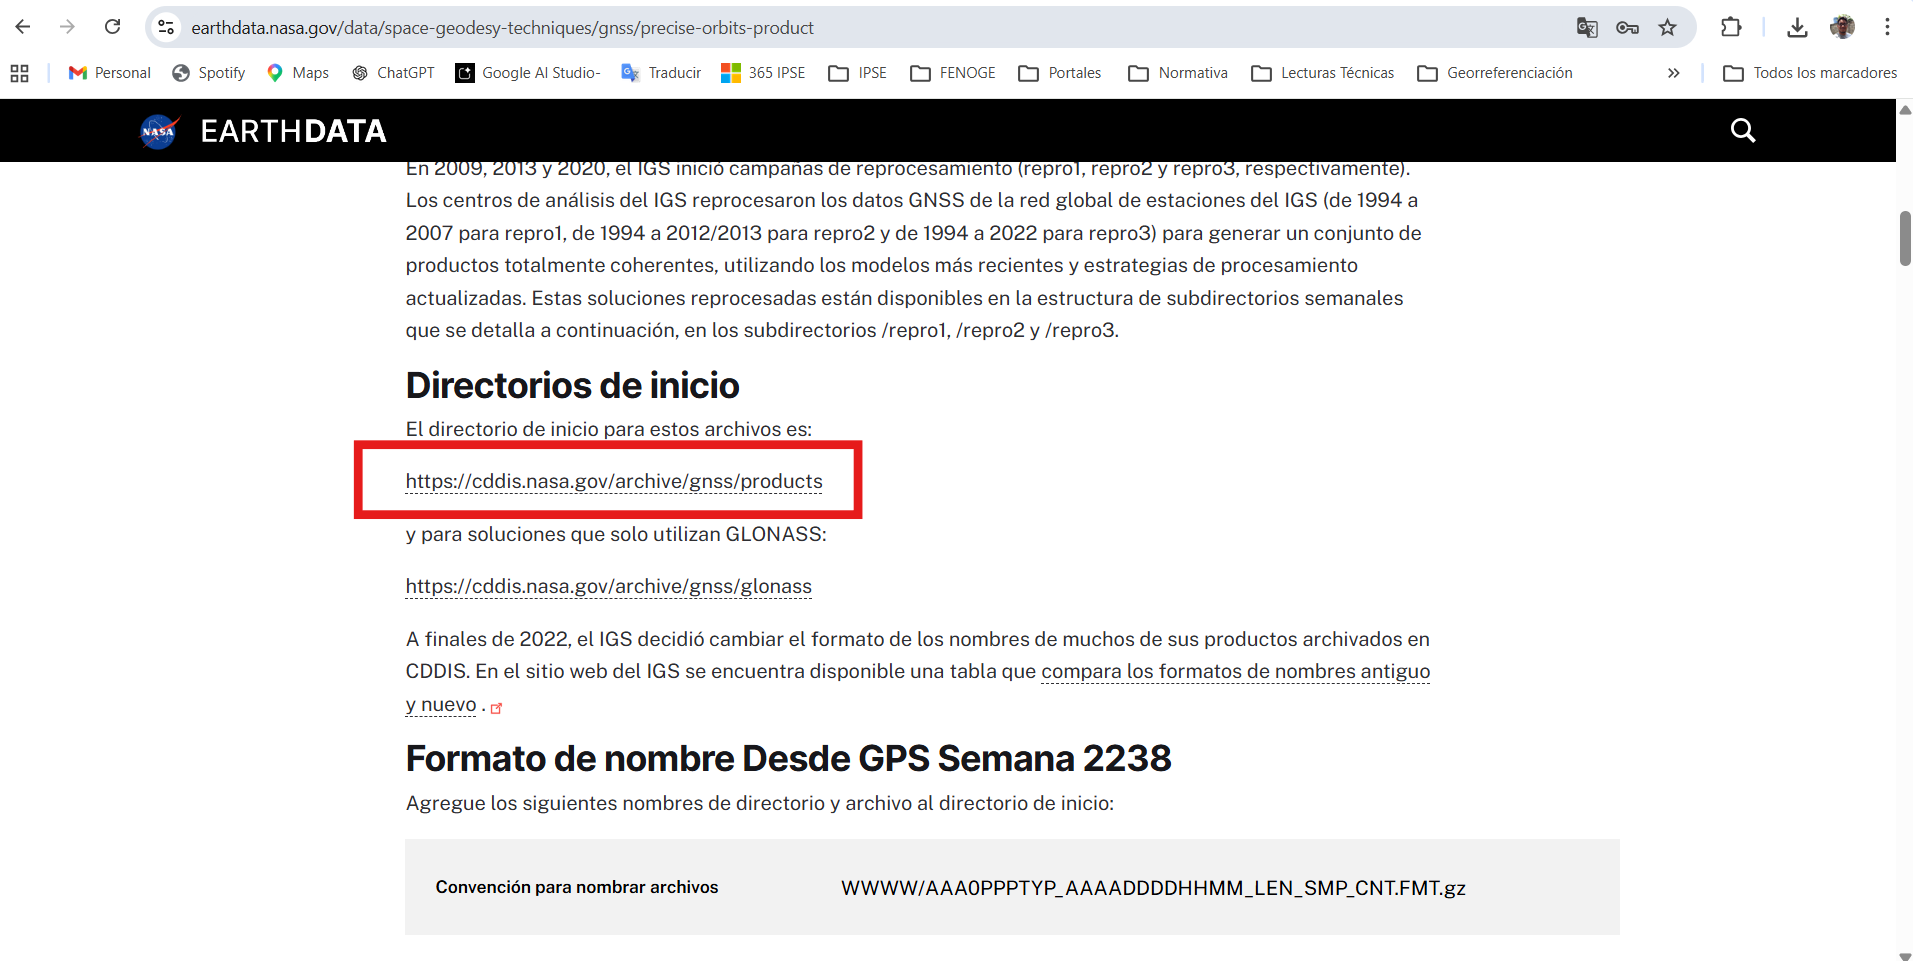
\includegraphics{./53-practica_13_gnss_allynav_r26_files/efemerides_precisas0.png}

}

\caption{Descarga de efemérides precisas Acceso a carpetas}

\end{figure}%%
\begin{figure}[H]

{\centering 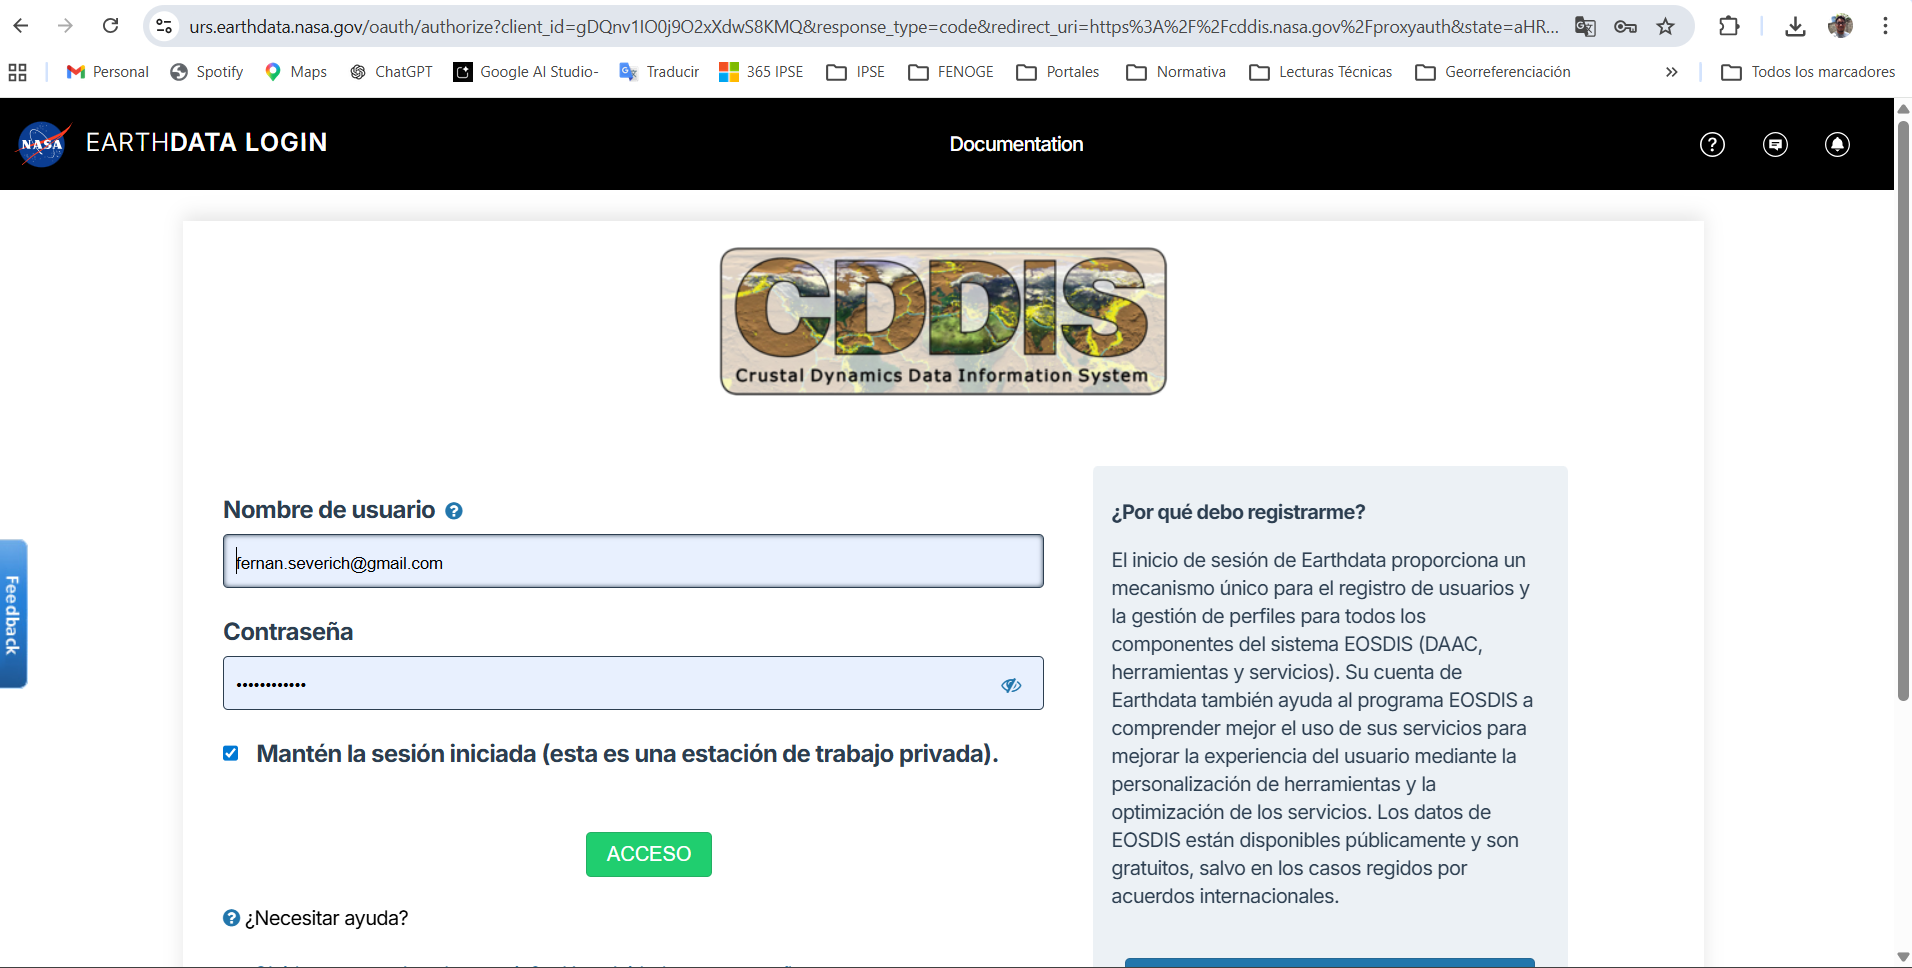
\includegraphics{./53-practica_13_gnss_allynav_r26_files/efemerides_precisas1.png}

}

\caption{Descarga de efemérides precisas Registro}

\end{figure}%%
\begin{figure}[H]

{\centering 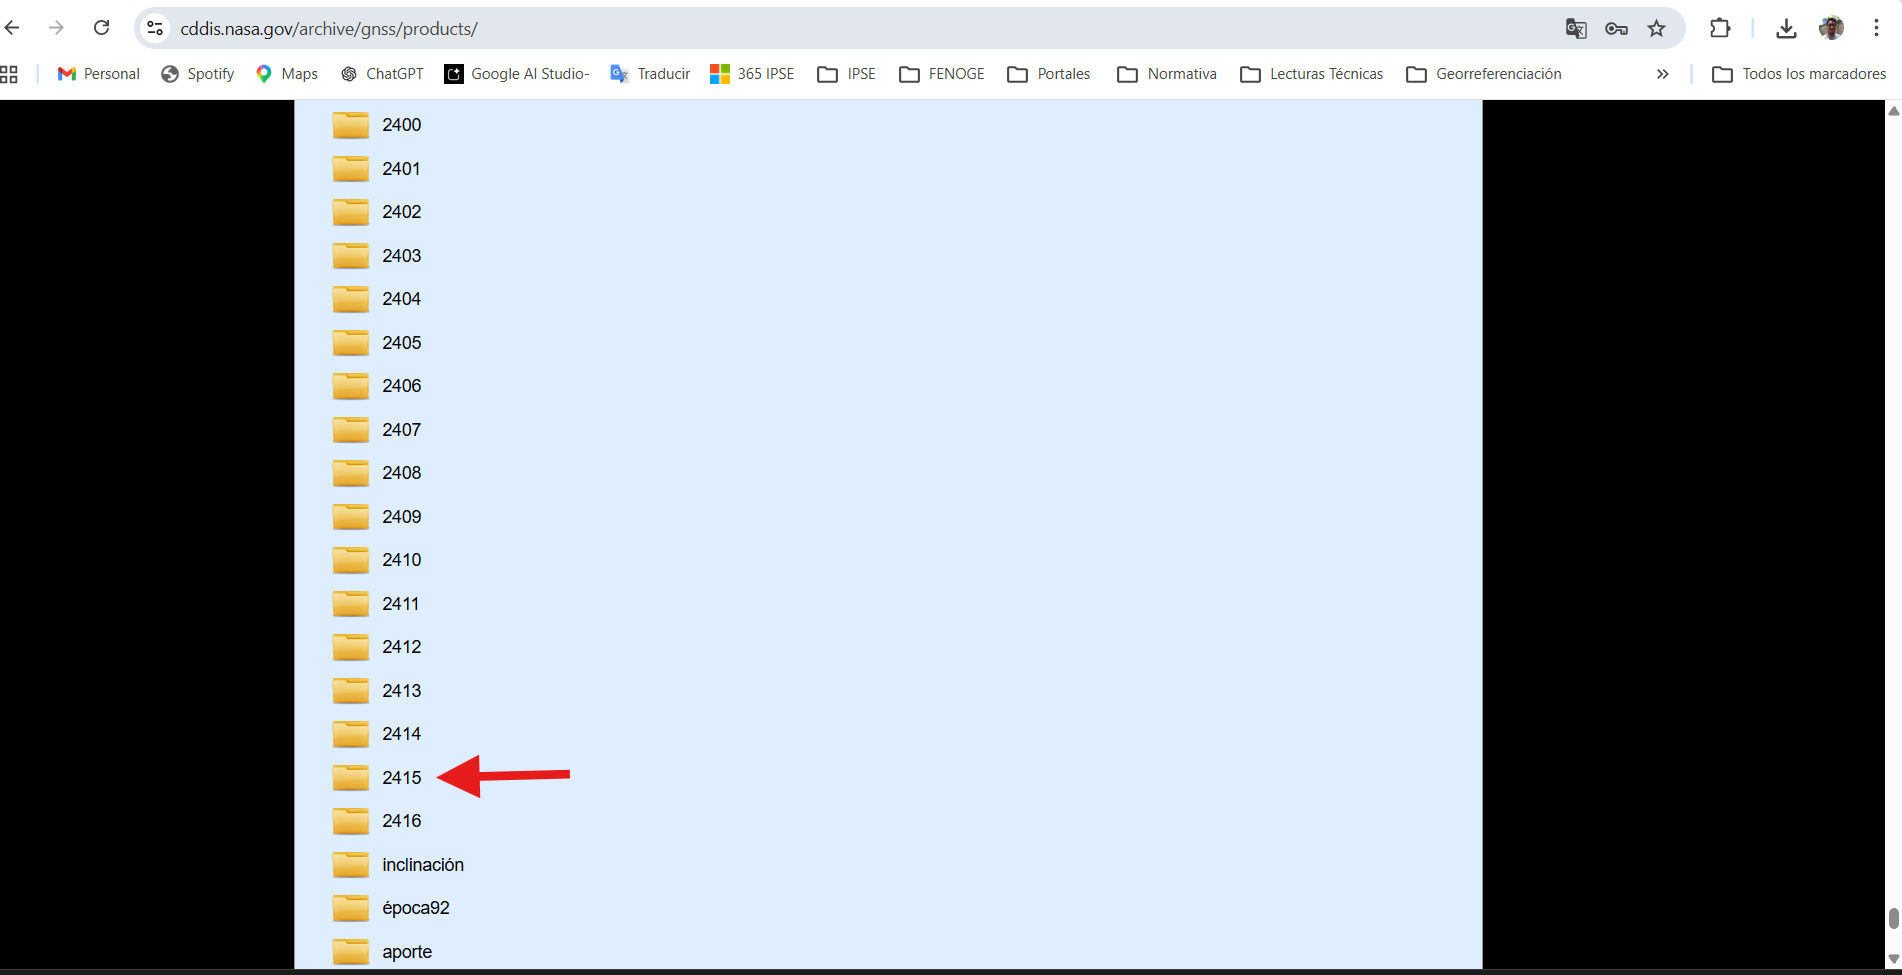
\includegraphics{./53-practica_13_gnss_allynav_r26_files/efemerides_precisas2.png}

}

\caption{Descarga de efemérides precisas busqueda semana GPS}

\end{figure}%%
\begin{figure}[H]

{\centering 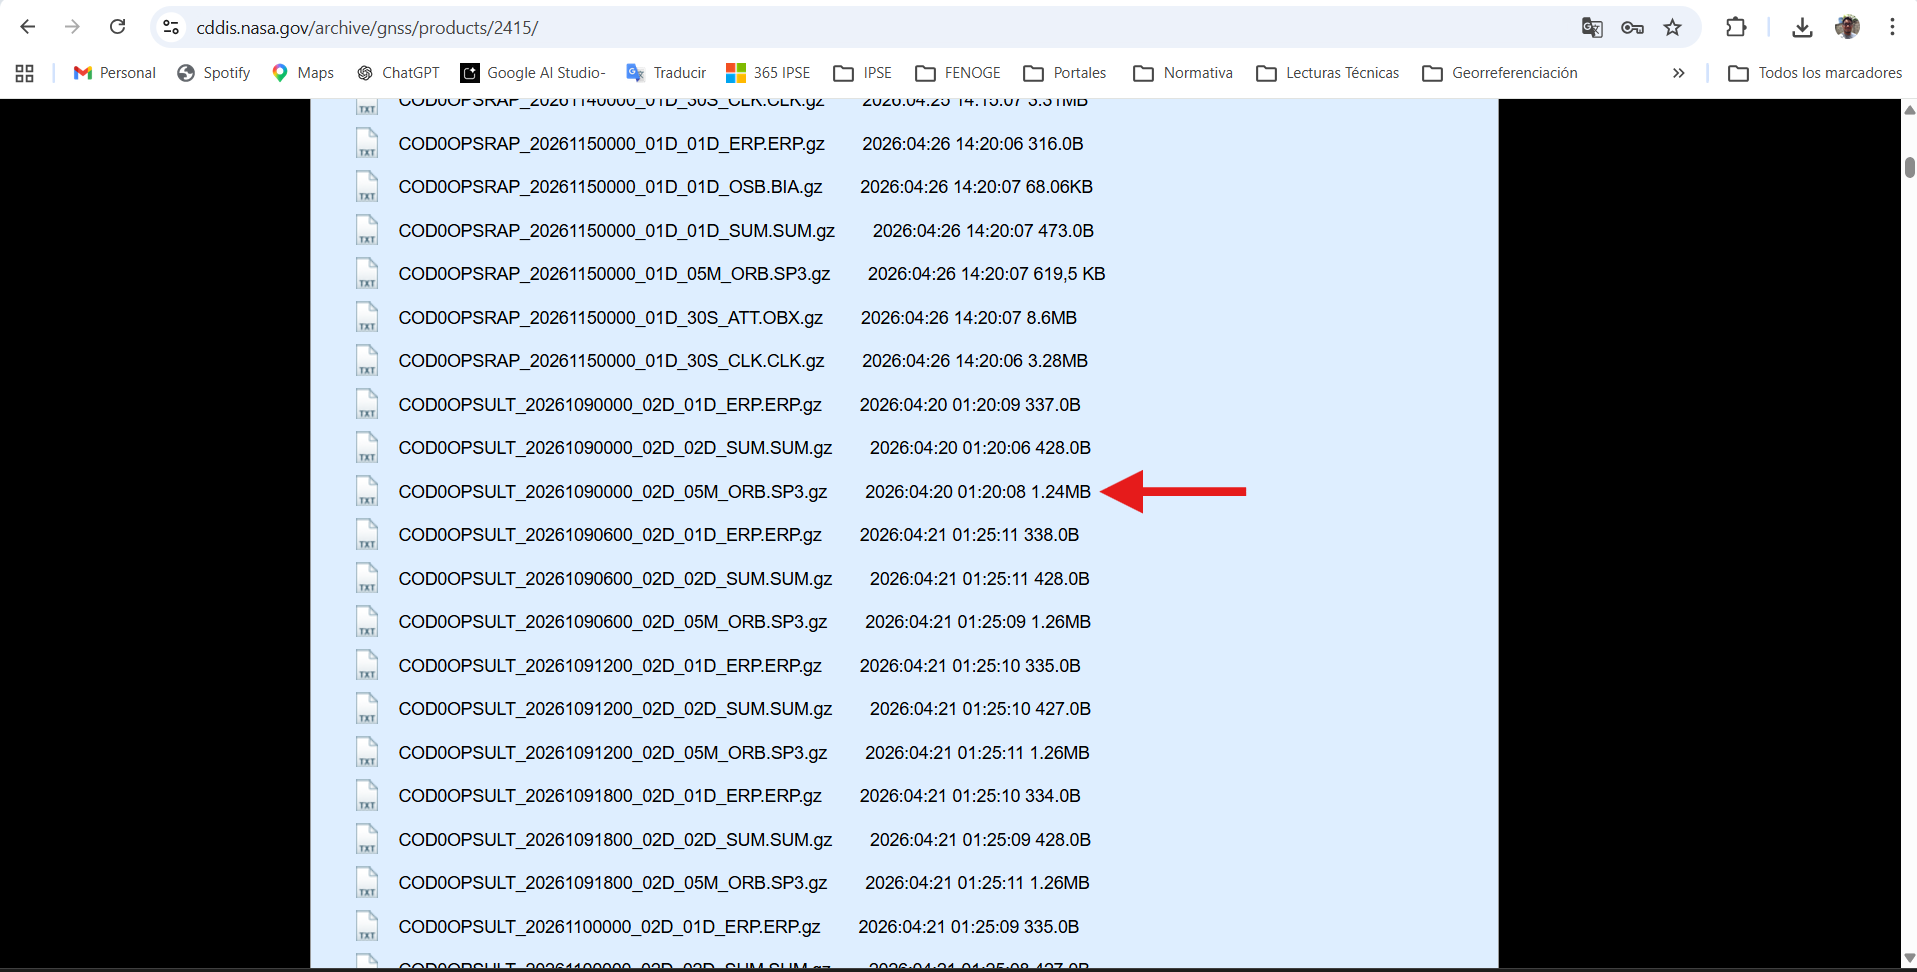
\includegraphics{./53-practica_13_gnss_allynav_r26_files/efemerides_precisas3.png}

}

\caption{Descarga de efemérides precisas a descargar}

\end{figure}%%
\begin{figure}[H]

{\centering 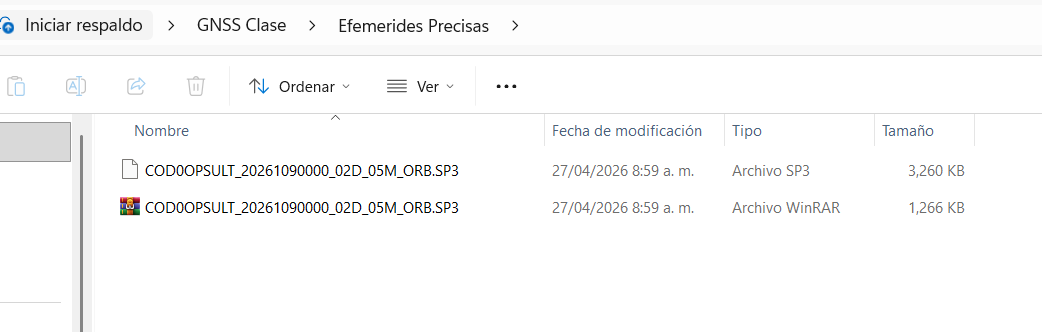
\includegraphics{./53-practica_13_gnss_allynav_r26_files/efemerides_precisas4.png}

}

\caption{Descarga de efemérides precisas descargadas}

\end{figure}%

\subsection{Postproceso del levantamiento
estático}\label{postproceso-del-levantamiento-estuxe1tico}

Con los archivos del punto observado, los archivos RINEX de la estación
permanente del IGAC, las efemérides precisas y la información de campo
debidamente organizada, se procede a realizar el postproceso del
levantamiento estático.

El procesamiento puede realizarse mediante diferentes aplicaciones
especializadas. En esta práctica se mostrará inicialmente el
procedimiento en una aplicación de libre acceso denominada \textbf{Emlid
Studio}, la cual permite realizar postproceso GNSS de manera sencilla.
Sin embargo, debe tenerse en cuenta que esta aplicación no permite
incorporar efemérides precisas dentro del procesamiento.

Descarga Emlid Studio: https://emlid.com/es/emlid-studio/

Posteriormente, se realizará el procesamiento en \textbf{RTKLIB},
mediante el módulo \textbf{RTKPOST}, el cual permite cargar archivos de
observación, navegación y efemérides precisas. Esto permitirá comparar
los resultados obtenidos con ambos procedimientos y analizar la
influencia de los insumos utilizados en la coordenada final procesada.

Descarga RTKLIB:
https://github.com/tomojitakasu/RTKLIB\_bin/tree/rtklib\_2.4.3

El objetivo de esta etapa es obtener una coordenada ajustada para la
base observada durante la práctica. Esta coordenada servirá como
referencia para revisar o corregir posteriormente las coordenadas del
levantamiento cinemático RTK del borde de vía.

\subsubsection{Postproceso del levantamiento estático Emlid
Studio.}\label{postproceso-del-levantamiento-estuxe1tico-emlid-studio.}

Se debe seleccionar el tipo de postproceso a realizar en la aplicación:
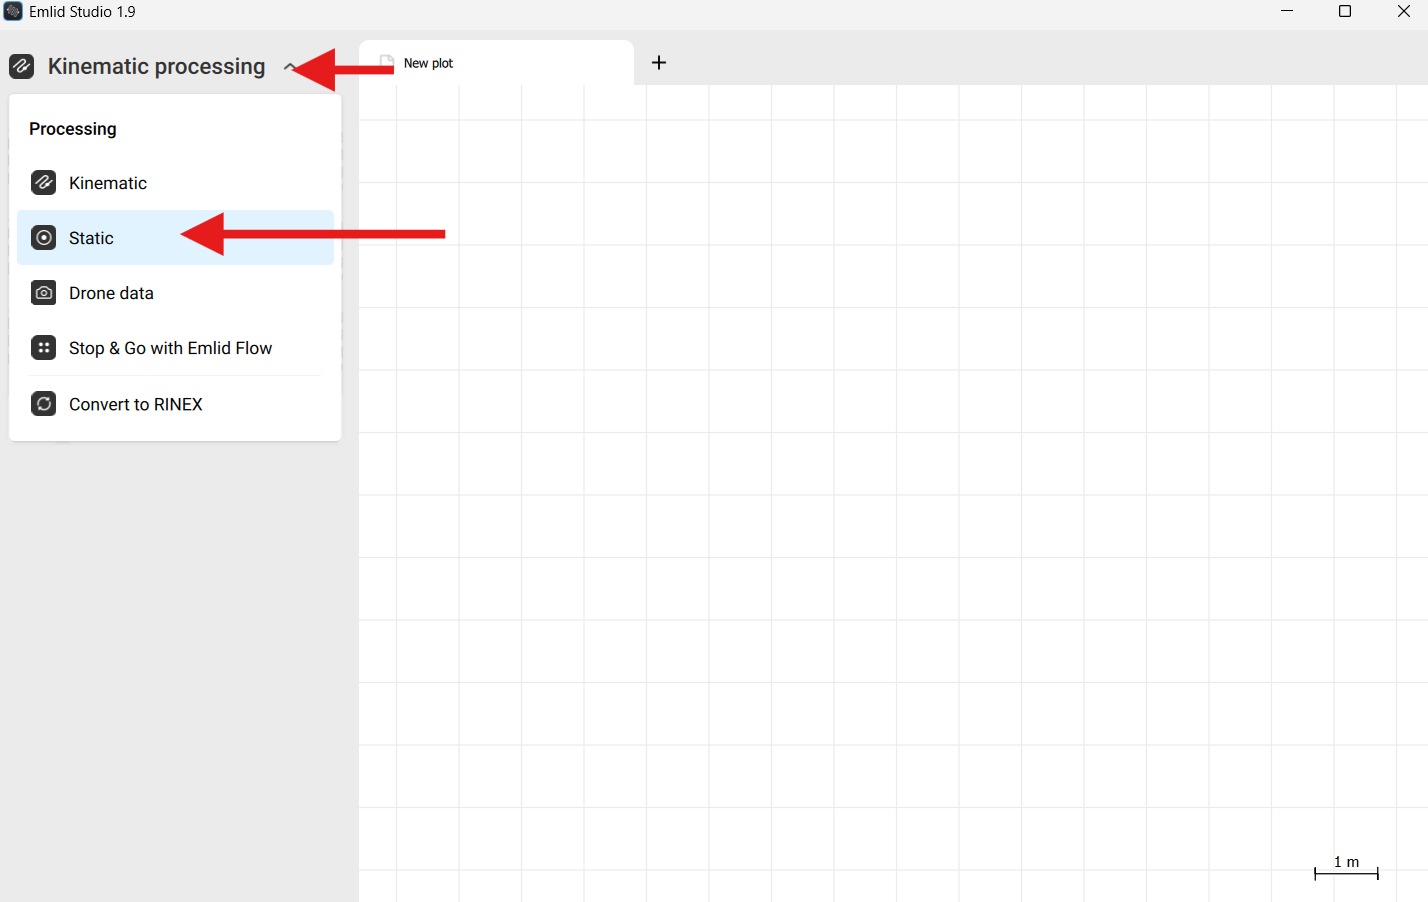
\includegraphics{./53-practica_13_gnss_allynav_r26_files/Emlid1.png}

Se importan o cargan los RINEX observados en nuestro levantamiento
Estático.

\begin{figure}[H]

{\centering 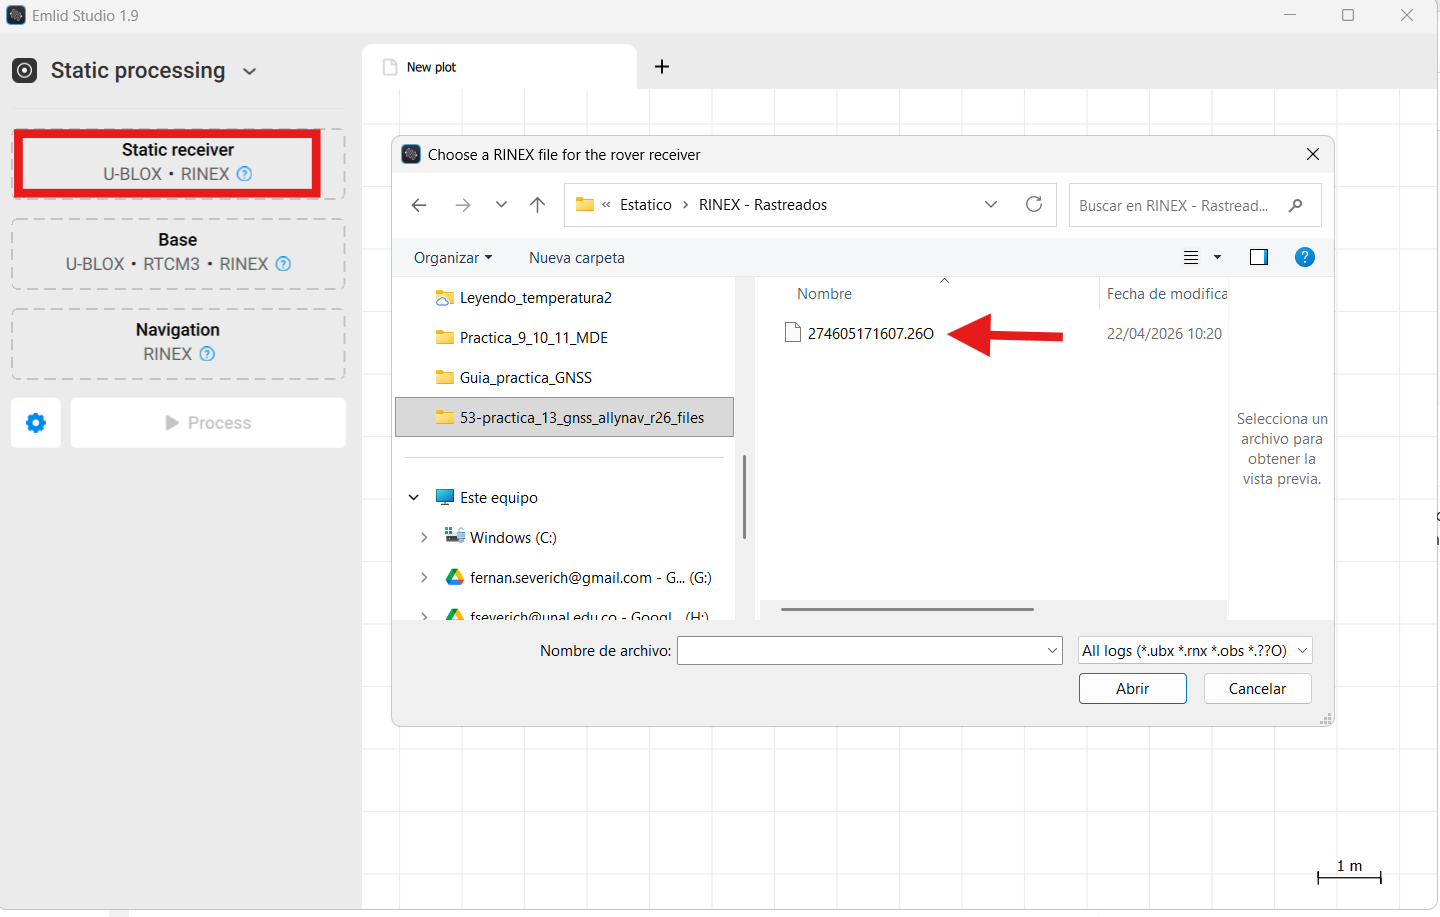
\includegraphics{./53-practica_13_gnss_allynav_r26_files/Emlid2.png}

}

\caption{Importación del archivo RINEX observados en vertive DOOF UNAL}

\end{figure}%

Debido a que durante la descarga de la los archivos RINEX de la base
BOGA, se descargaron archivos D, N, G, siendo D, el archivo de
observaciones O, la aplicación Emlid Studio no reconoce este archivo.
Por tanto es necesario realizar la descarga de los archivos rinex 3.11
de la pagina del IGAC

\begin{figure}[H]

{\centering 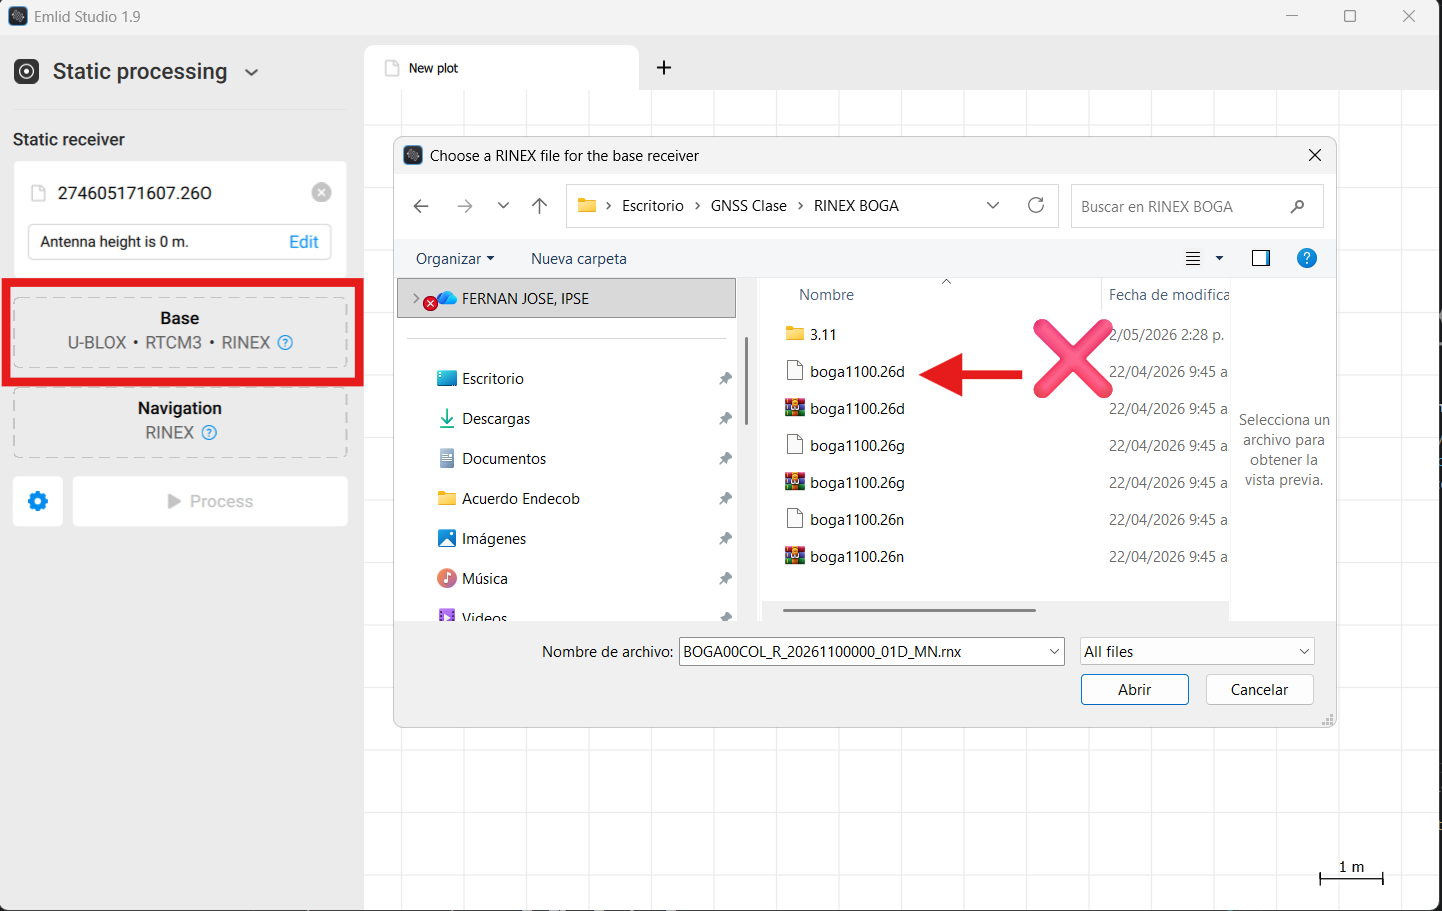
\includegraphics{./53-practica_13_gnss_allynav_r26_files/Emlid3.png}

}

\caption{Cargue de archivos RINEX de Base - Fallida por archivo D}

\end{figure}%

Notese que ahora solo son dos archivos a descargar.

\begin{figure}[H]

{\centering 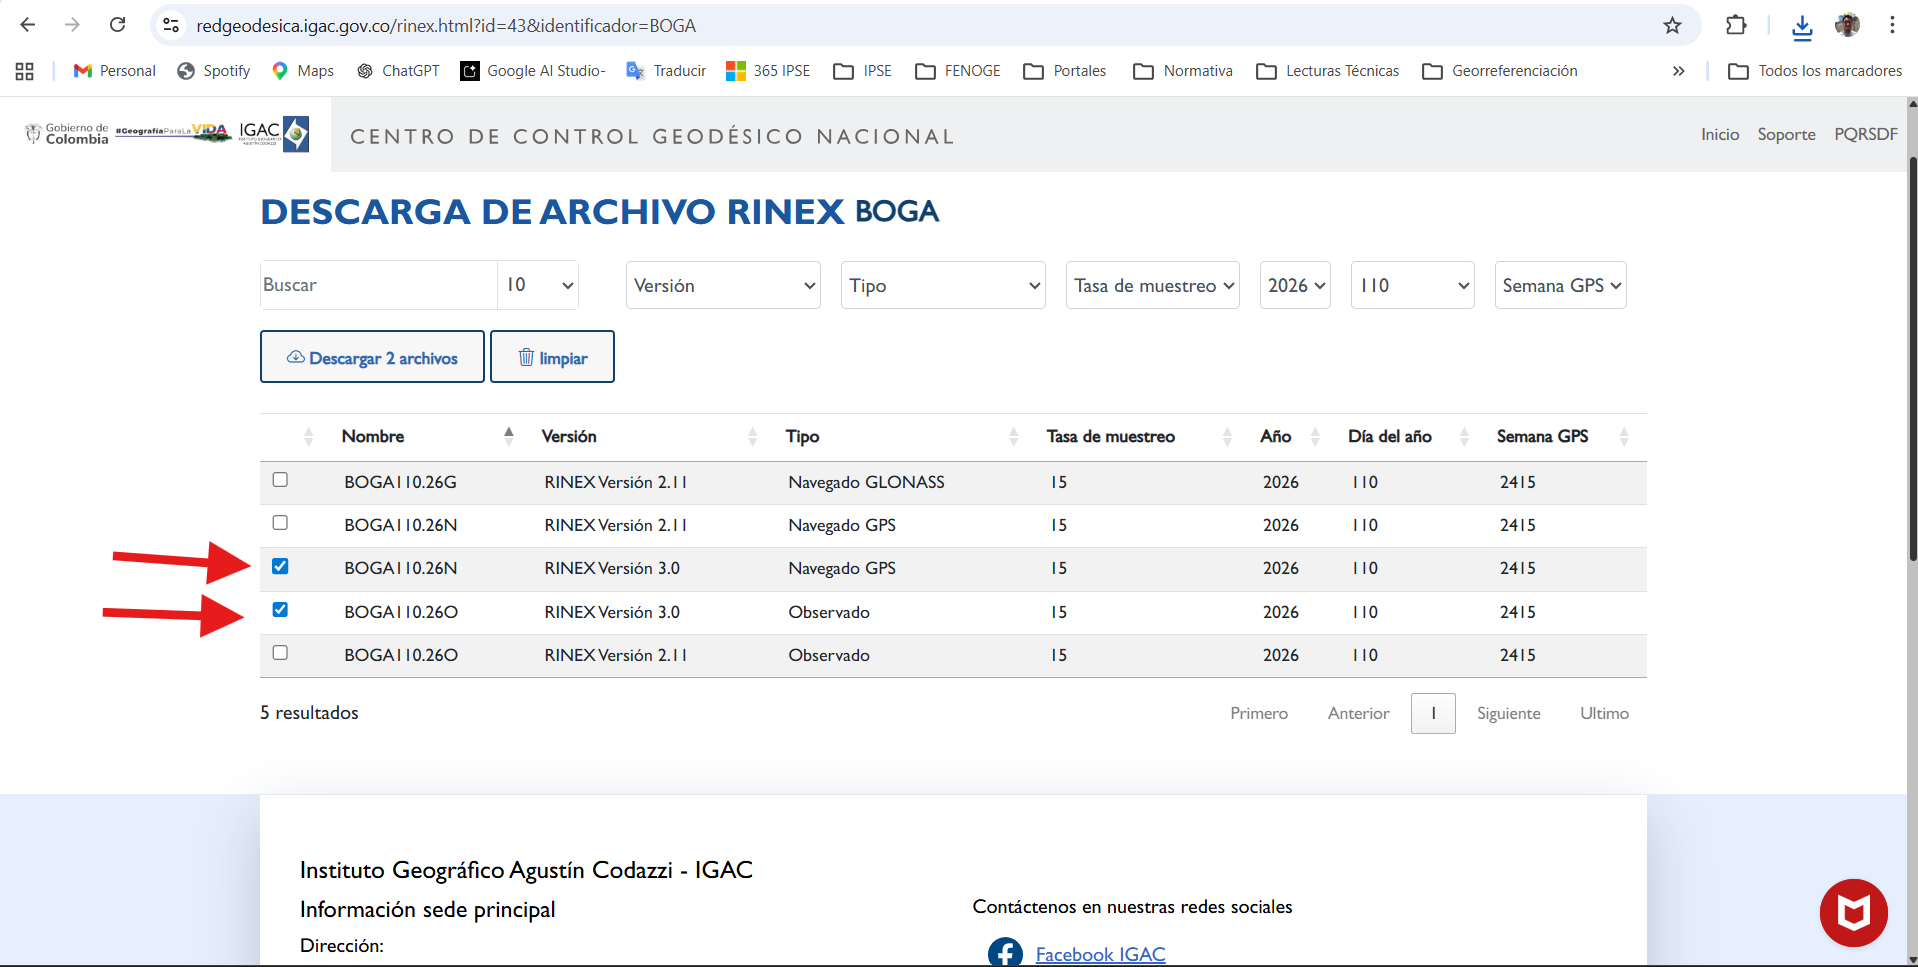
\includegraphics{./53-practica_13_gnss_allynav_r26_files/Emlid4.png}

}

\caption{Descarga de RINEX estación BOGA Formato 3.11}

\end{figure}%

Adicionalmente se recomienda realizar la conversion del archivo crudo
del levantamiento estático a RINEX 3.01

\begin{figure}[H]

{\centering 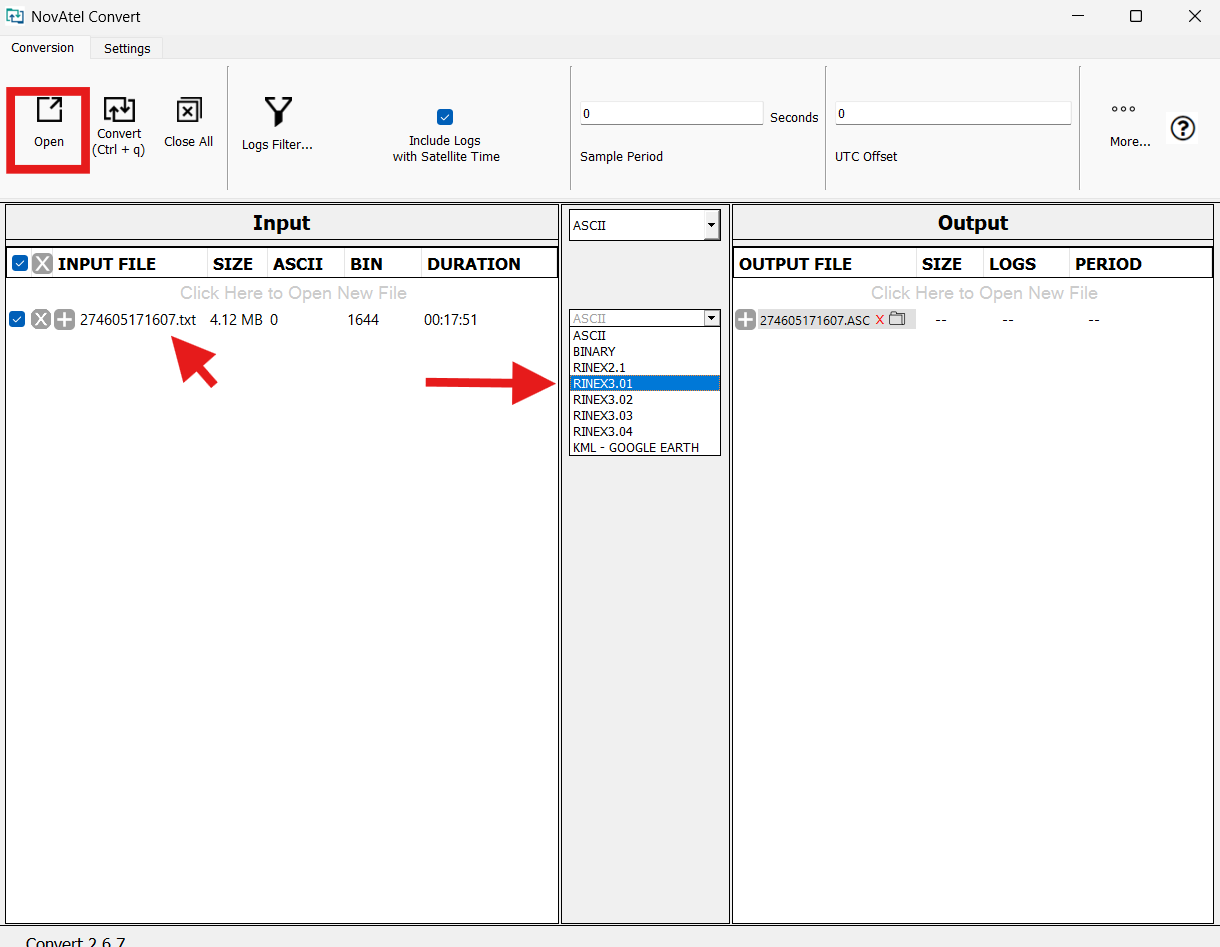
\includegraphics{./53-practica_13_gnss_allynav_r26_files/Emlid5.png}

}

\caption{Conversion de archivos brutos a RINEX 3.01}

\end{figure}%

Se puede observar en la siguiente imagen que los archivos RINEX
observados en formato 3.11, la extensión del archivo es .rnx

\begin{figure}[H]

{\centering 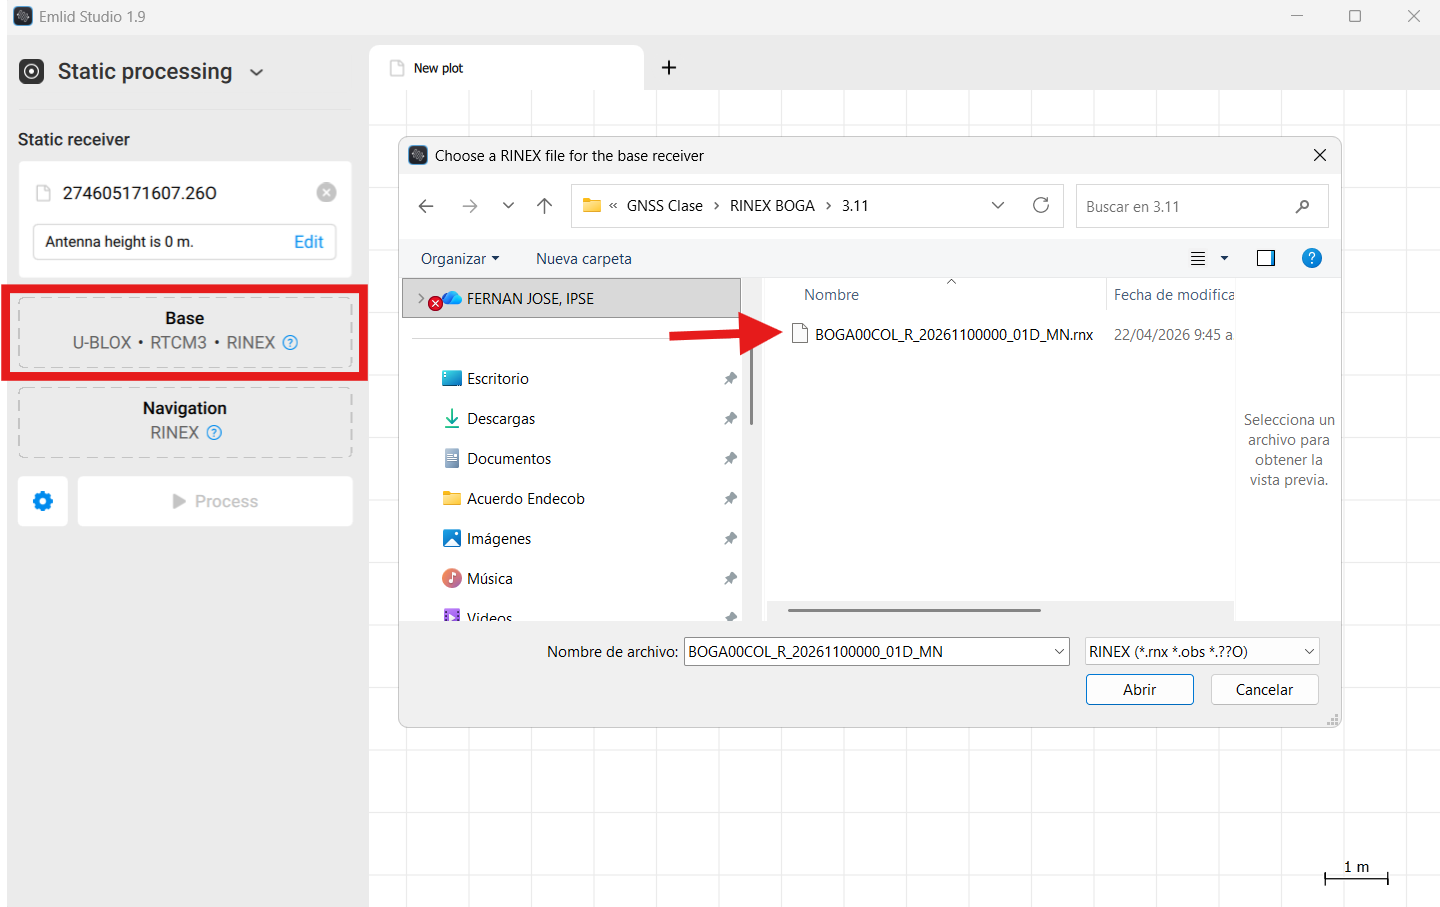
\includegraphics{./53-practica_13_gnss_allynav_r26_files/Emlid6.png}

}

\caption{Cargue de Archivos RINEX 3.11 de estacion Base IGAC - BOGA}

\end{figure}%%
\begin{figure}[H]

{\centering 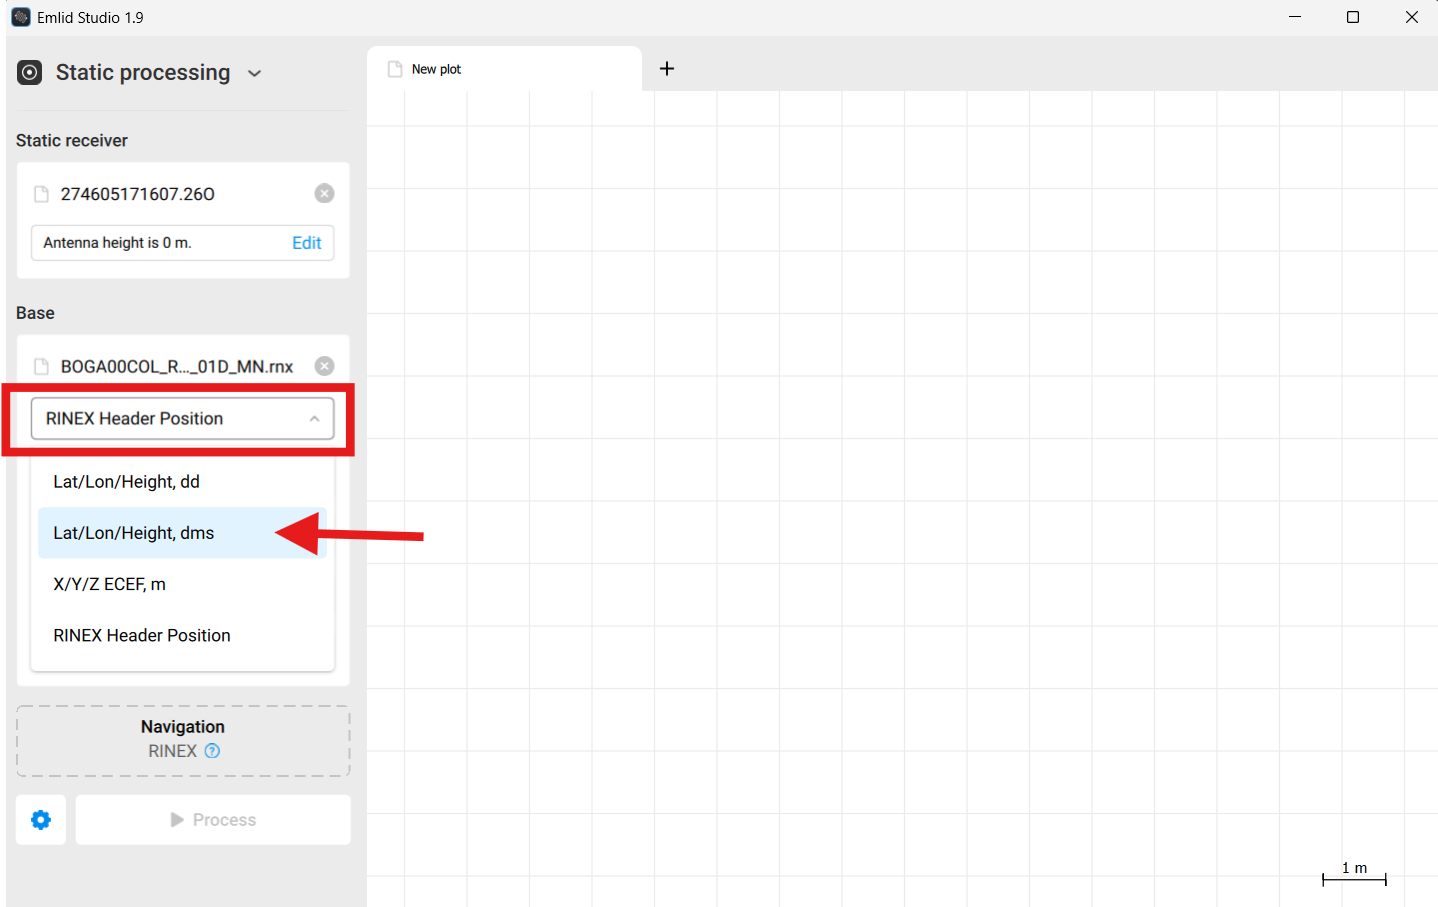
\includegraphics{./53-practica_13_gnss_allynav_r26_files/Emlid7.png}

}

\caption{Definir coordenadas de la base permanente BOGA}

\end{figure}%

Estas coordenadas a ingresar de la base se localizan en la misma pagina
de la red geodesica nacional - Red activa GNSS - Filtrando BOGA -
Detalles. Estas se rellenan en los espacios de la aplicación, incluyendo
la altura de la antena que tambien se reporta en la página.

\begin{figure}[H]

{\centering 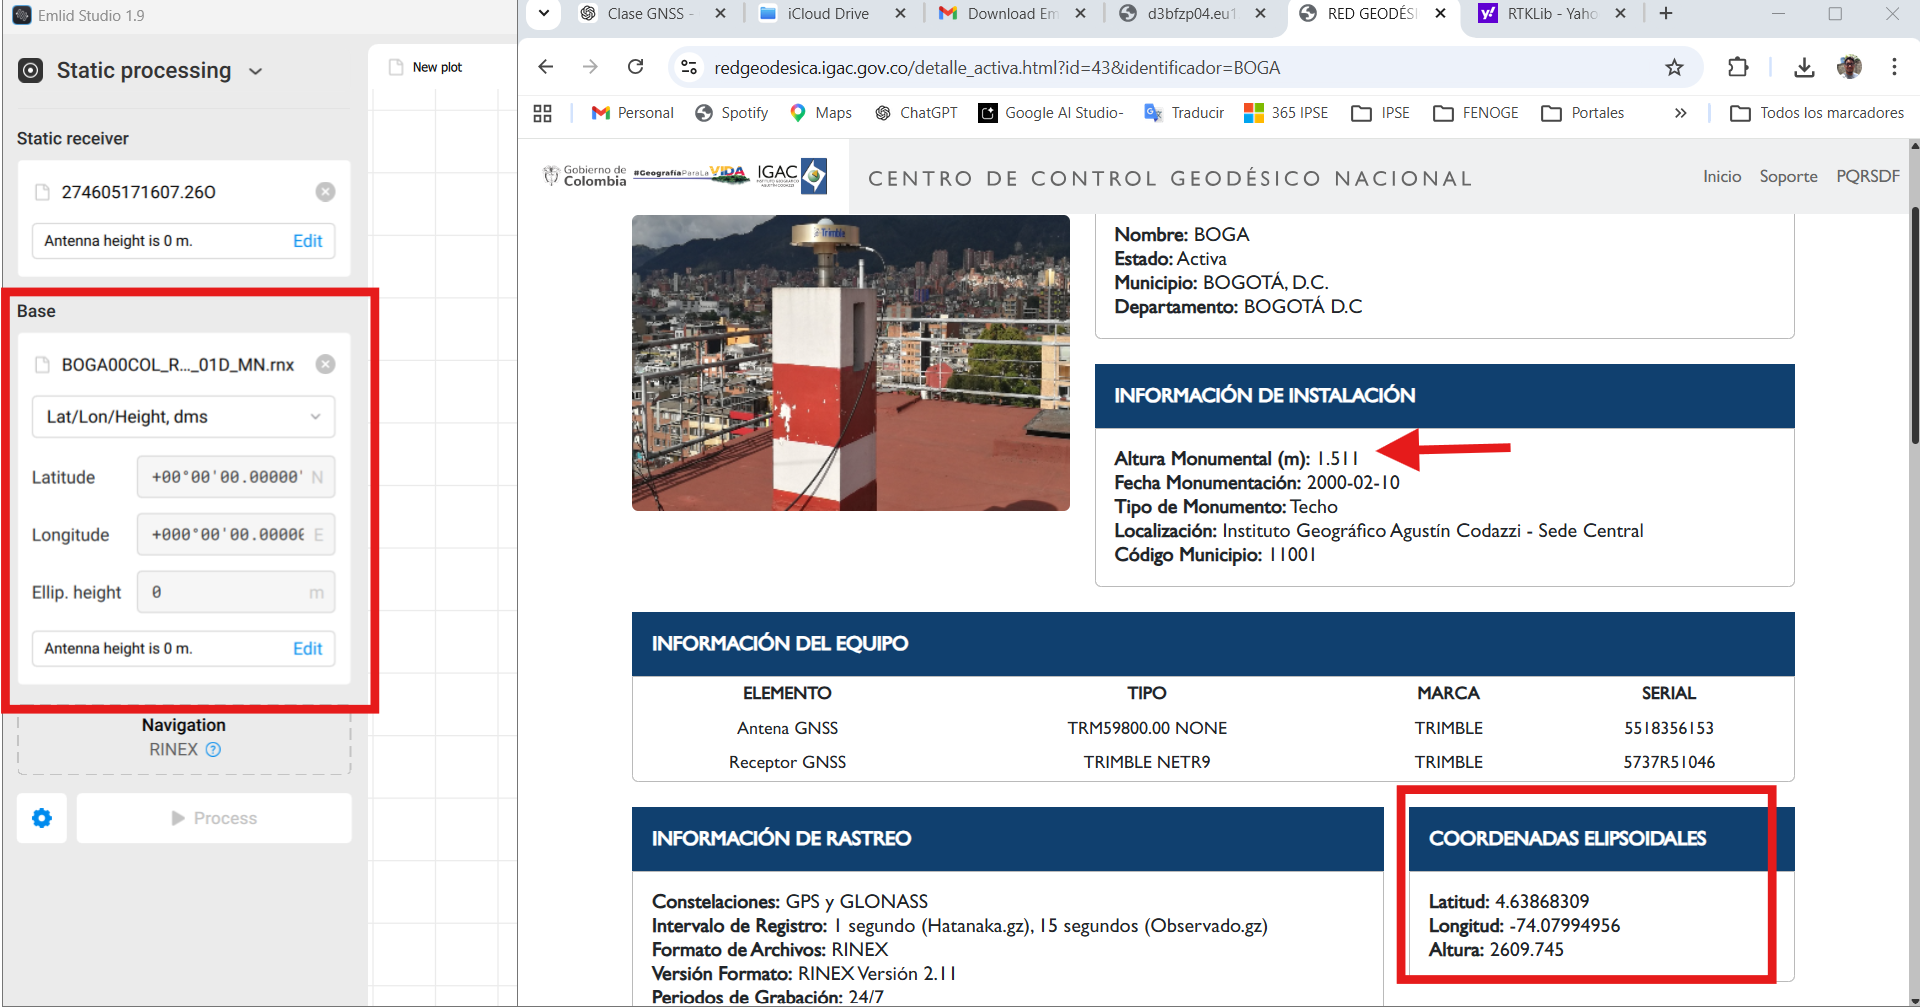
\includegraphics{./53-practica_13_gnss_allynav_r26_files/Emlid8.png}

}

\caption{Configuración de altura de antena y tipo de medición}

\end{figure}%

No olvidar tambien introducir la altura de la antena de nuestro equipo
sobre vertice DOOf UNAL:

\begin{figure}[H]

{\centering 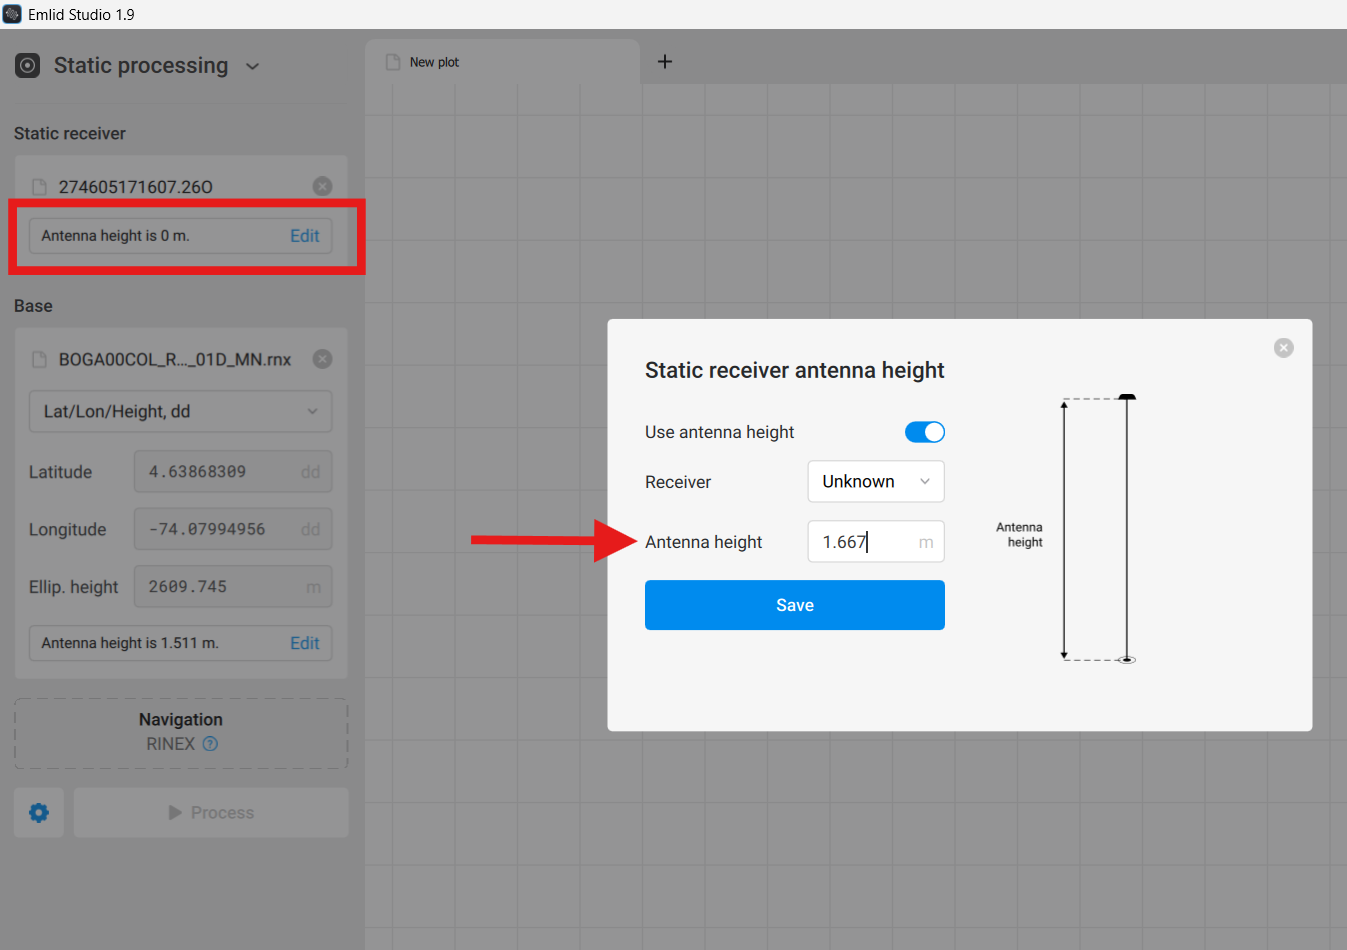
\includegraphics{./53-practica_13_gnss_allynav_r26_files/Emlid9.png}

}

\caption{Altura de la Antena en vertice DOOF UNAL - Observado}

\end{figure}%

Se cargan los archivos navegados de la estación Base BOGA:

\begin{figure}[H]

{\centering 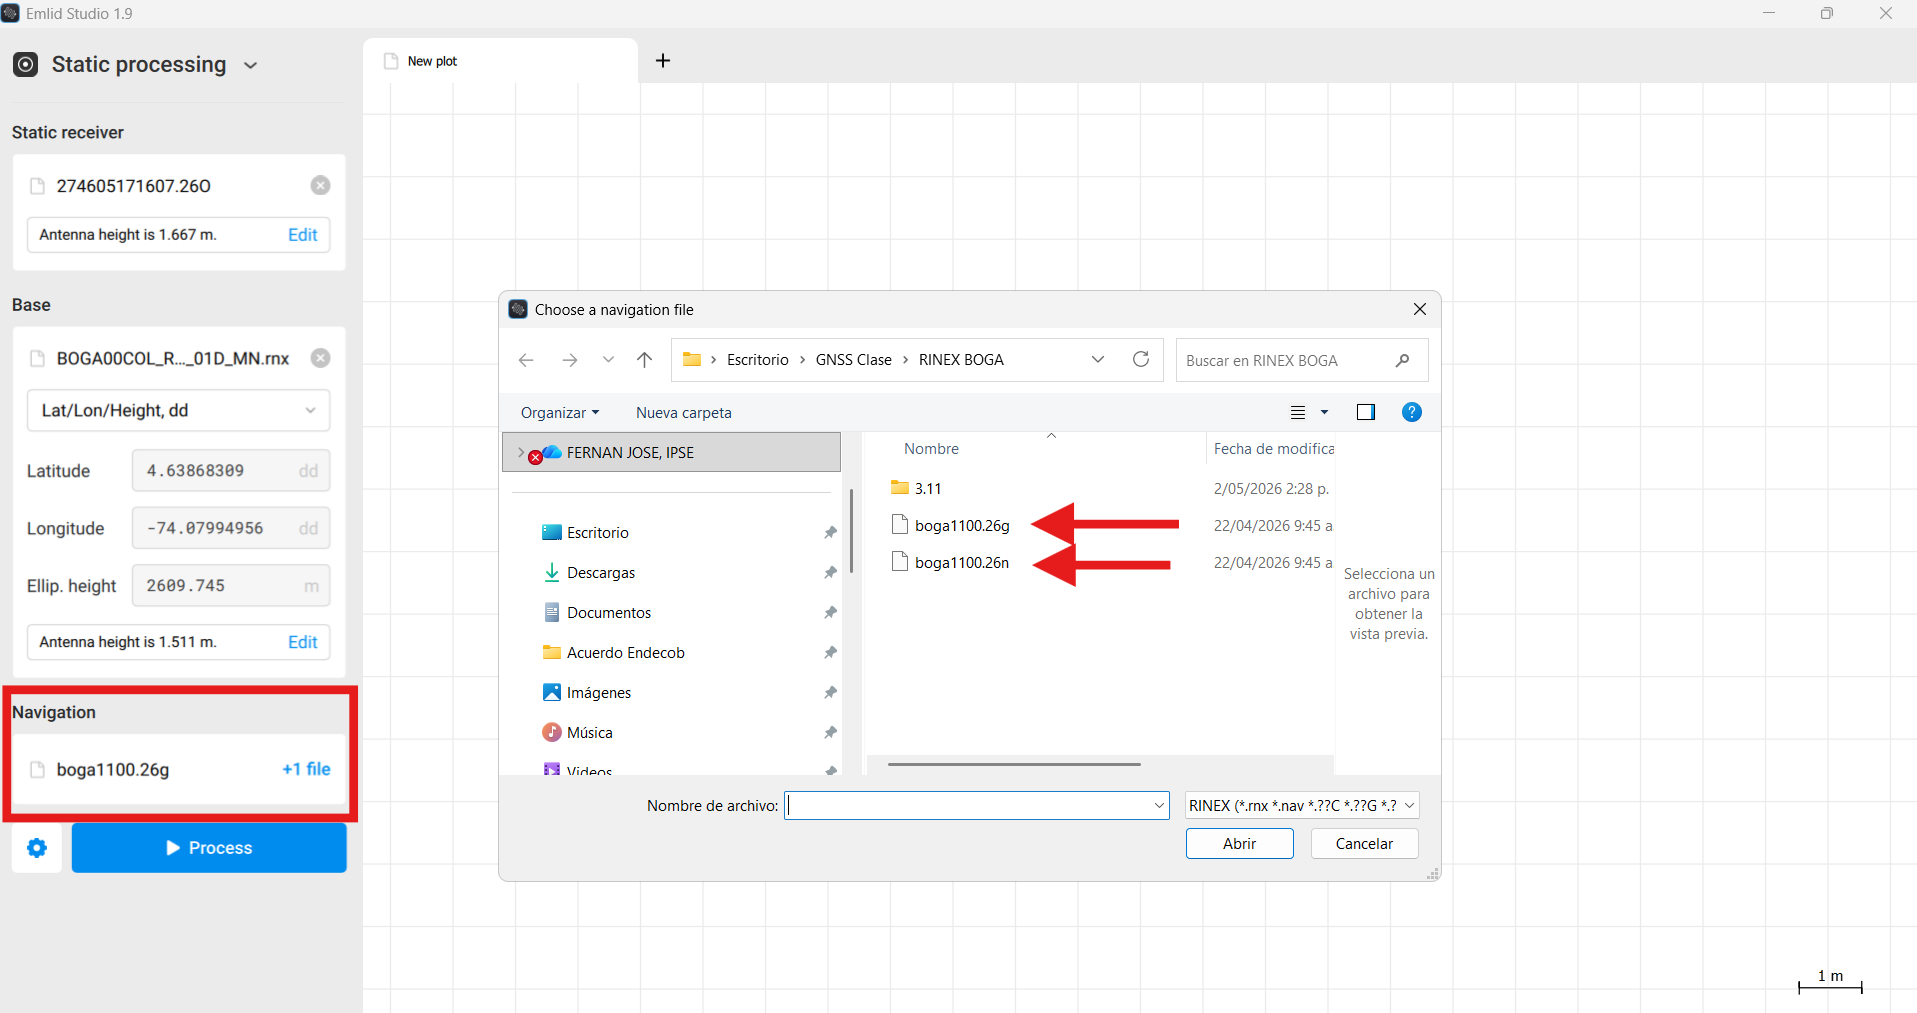
\includegraphics{./53-practica_13_gnss_allynav_r26_files/Emlid10.png}

}

\caption{Cargue de archivos navegados N, G, de la estación Base
PErmanente BOGA}

\end{figure}%

Se realizan configuraciones adicionales, como cambiar la ruta de
guardado y nombre del archivo resultado del postproceso, el lapso de
tiempo del levantamiento (para este dato se puede abrir los archivos de
observacion y ver los tiempos), tambien se pueden modificar las
constelaciones de satelites a procesar (GPS, GLONASS, GALILEO, BEIDOU,
SBAS\ldots etc) el formato de salida de coordenadas y tiempo.

\begin{figure}[H]

{\centering 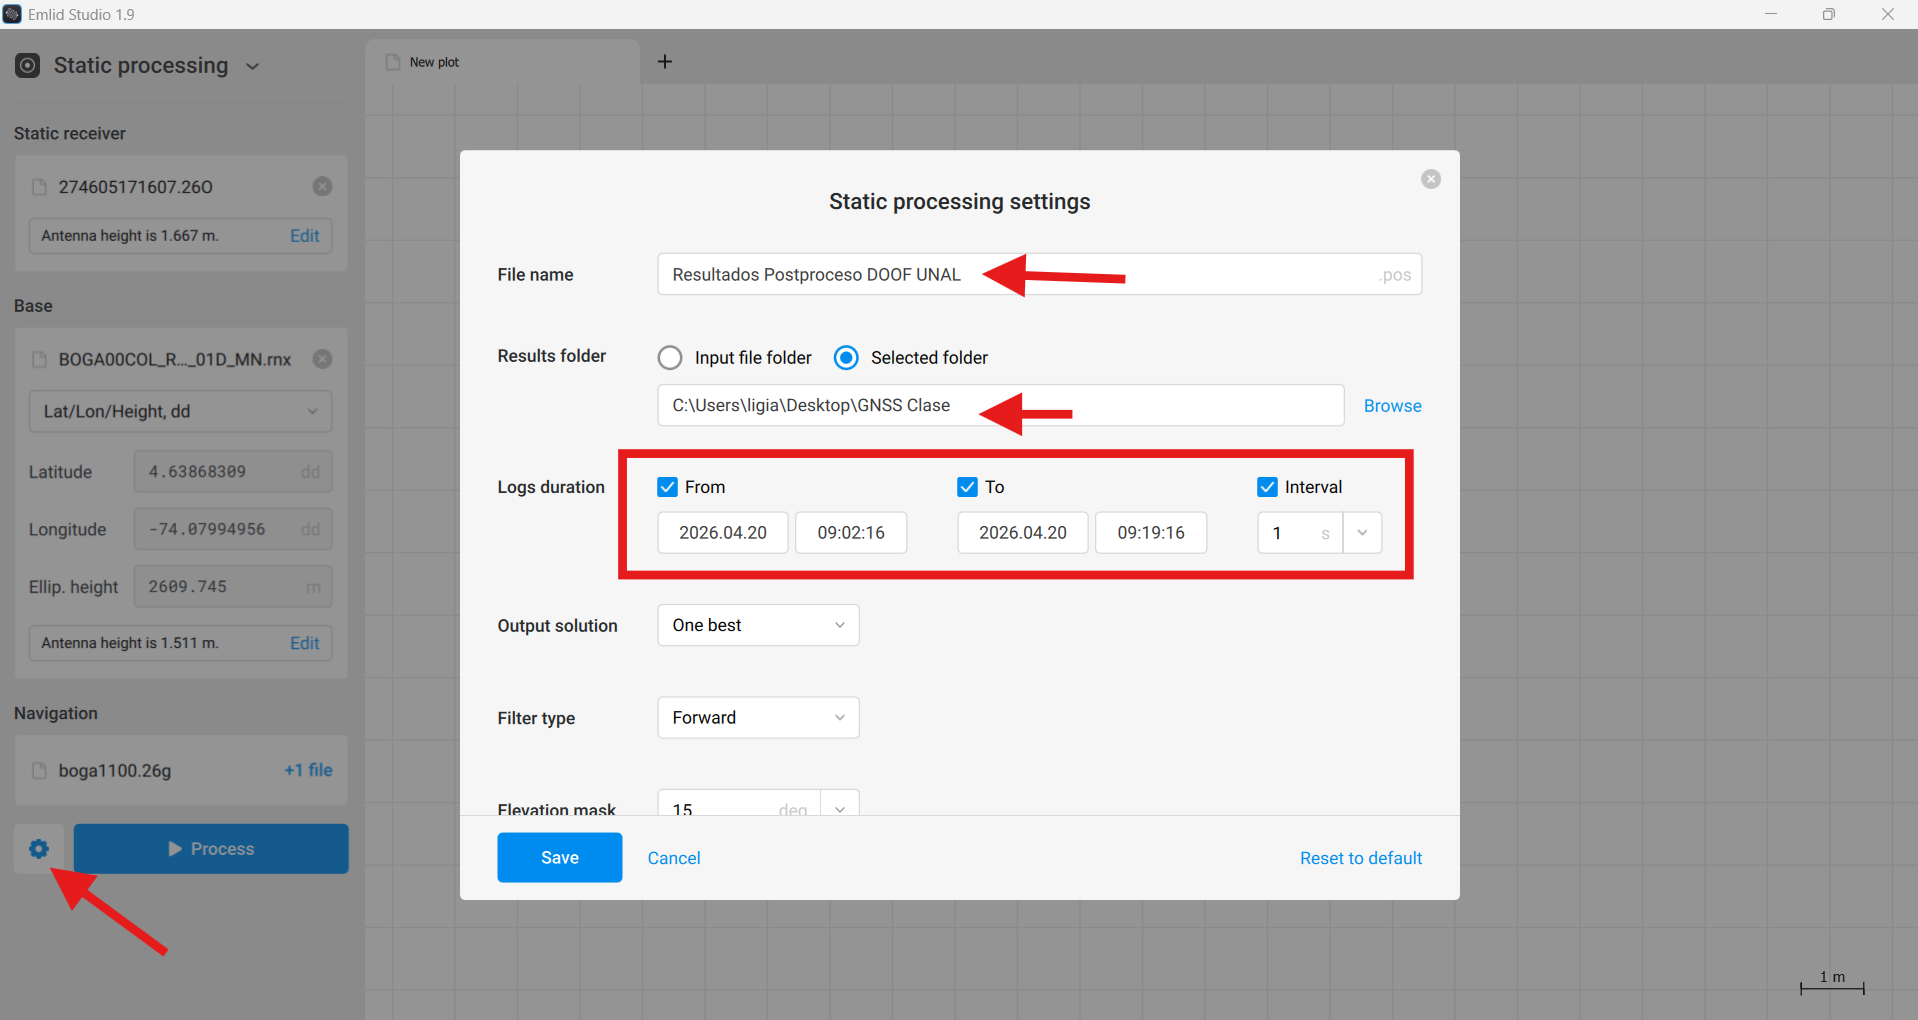
\includegraphics{./53-practica_13_gnss_allynav_r26_files/Emlid11.png}

}

\caption{Cargue de archivos navegados N, G, de la estación Base
Permanente BOGA}

\end{figure}%

\subsubsection{Postproceso del levantamiento estático con
RTKLIB}\label{postproceso-del-levantamiento-estuxe1tico-con-rtklib}

RTKLIB - Trae la aplicación de RTKPOST para realizar postproceso.
RTKPOST permite procesar observaciones GNSS diferenciales a partir de un
punto observado y una estación base de referencia. Para esta práctica,
el punto observado corresponde al receptor instalado sobre el vértice
geodésico de la Universidad Nacional, mientras que la estación base
corresponde a la estación permanente \textbf{BOGA} del IGAC.

\textbf{Configuración inicial de RTKPOST}: Al abrir RTKPOST se despliega
la ventana principal del aplicativo. En esta ventana se deben activar
las casillas \textbf{Time Start} y \textbf{Time End}, correspondientes
al tiempo de inicio y finalización del rastreo estático.

Para esta práctica, el levantamiento fue realizado el día \textbf{20 de
abril de 2026}. Al revisar los archivos de observación, se identifica
que el rastreo inició a las \textbf{14:02:16 GPST} y finalizó a las
\textbf{14:20:07 GPST}. Por tanto, estos son los valores que deben
ingresarse en la ventana inicial de RTKPOST.

El intervalo de procesamiento se configura en \textbf{1 segundo}, dado
que el levantamiento estático fue realizado con una frecuencia de
registro de \textbf{1 Hz}, equivalente a una observación por segundo.

\begin{figure}[H]

{\centering 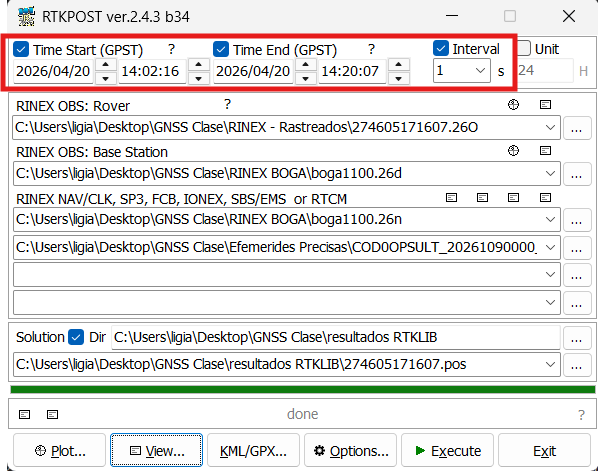
\includegraphics{./53-practica_13_gnss_allynav_r26_files/RTKLIB1.png}

}

\caption{Configuración de fecha, hora de inicio, hora final e intervalo
de procesamiento en RTKPOST}

\end{figure}%

En la ventana principal también se deben cargar los archivos de entrada
requeridos para el procesamiento:

\begin{longtable}[]{@{}
  >{\raggedright\arraybackslash}p{(\columnwidth - 4\tabcolsep) * \real{0.3333}}
  >{\raggedright\arraybackslash}p{(\columnwidth - 4\tabcolsep) * \real{0.3333}}
  >{\raggedright\arraybackslash}p{(\columnwidth - 4\tabcolsep) * \real{0.3333}}@{}}
\toprule\noalign{}
\begin{minipage}[b]{\linewidth}\raggedright
Campo en RTKPOST
\end{minipage} & \begin{minipage}[b]{\linewidth}\raggedright
Archivo a cargar
\end{minipage} & \begin{minipage}[b]{\linewidth}\raggedright
Descripción
\end{minipage} \\
\midrule\noalign{}
\endhead
\bottomrule\noalign{}
\endlastfoot
RINEX OBS: Rover & Archivo de observación del punto levantado &
Corresponde al RINEX del receptor ubicado sobre el vértice observado \\
RINEX OBS: Base Station & Archivo de observación de la estación BOGA &
Corresponde al RINEX de la estación permanente del IGAC \\
RINEX NAV/CLK, SP3, etc. & Archivo de navegación & Se carga el archivo
de navegación de la estación BOGA \\
RINEX NAV/CLK, SP3, etc. & Efemérides precisas & Se carga el archivo de
efemérides precisas descargado para la semana GNSS y día
correspondiente \\
\end{longtable}

\begin{figure}

\begin{minipage}{0.50\linewidth}

\centering{

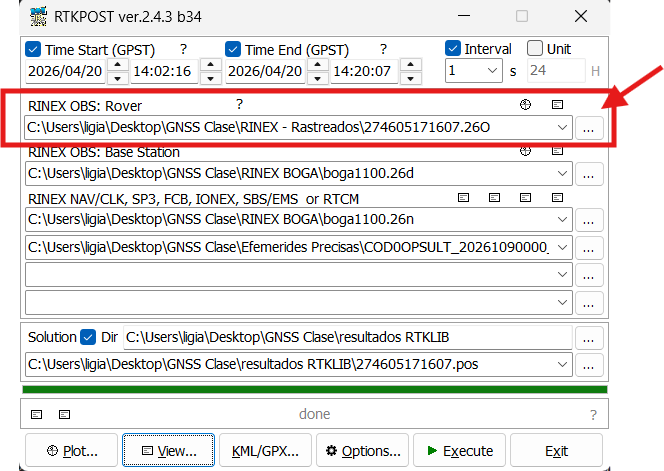
\includegraphics{53-practica_13_gnss_allynav_r26_files/RTKLIB2.png}

}

\subcaption{\label{fig-Vertice}RINEX observados sobre vertice DOOF UNAL}

\end{minipage}%
%
\begin{minipage}{0.50\linewidth}

\centering{

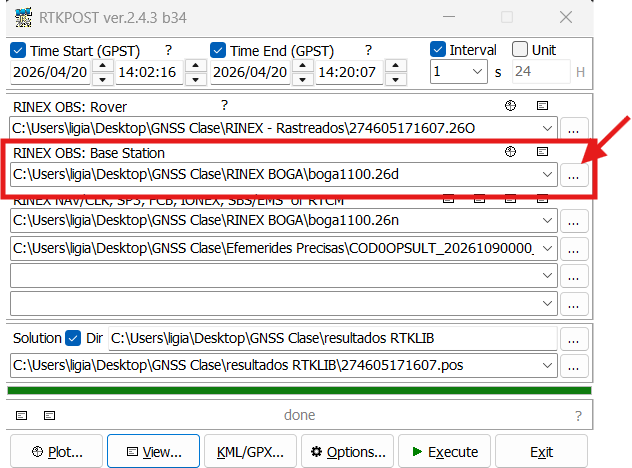
\includegraphics{53-practica_13_gnss_allynav_r26_files/RTKLIB3.png}

}

\subcaption{\label{fig-rover_V}RINEX de base permanente BOGA}

\end{minipage}%

\caption{\label{fig-RTKLIB}Fotos de app RTKPOST.}

\end{figure}%

\begin{figure}

\begin{minipage}{0.50\linewidth}

\centering{

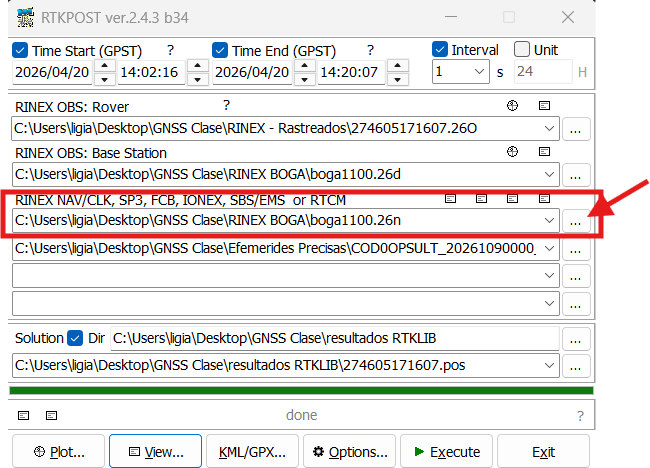
\includegraphics{53-practica_13_gnss_allynav_r26_files/RTKLIB4.png}

}

\subcaption{\label{fig-Vertice}RINEX Navegados de Base permanente BOGA}

\end{minipage}%
%
\begin{minipage}{0.50\linewidth}

\centering{

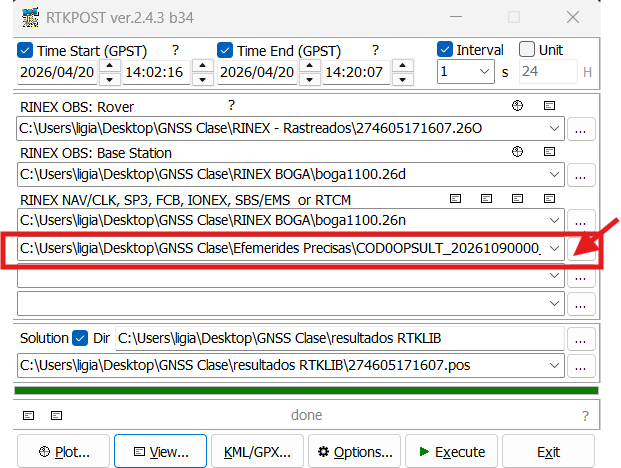
\includegraphics{53-practica_13_gnss_allynav_r26_files/RTKLIB5.png}

}

\subcaption{\label{fig-rover_V}Archivo de Efemérides Precisas}

\end{minipage}%

\caption{\label{fig-RTKLIB2}Fotos de app RTKPOST.}

\end{figure}%

En la sección \textbf{Solution}, se selecciona la carpeta donde se
guardarán los resultados del procesamiento. RTKPOST genera un archivo de
salida con extensión \texttt{.pos}, en el cual se almacenan las
coordenadas resultantes y la información de calidad de la solución.

\begin{figure}[H]

{\centering 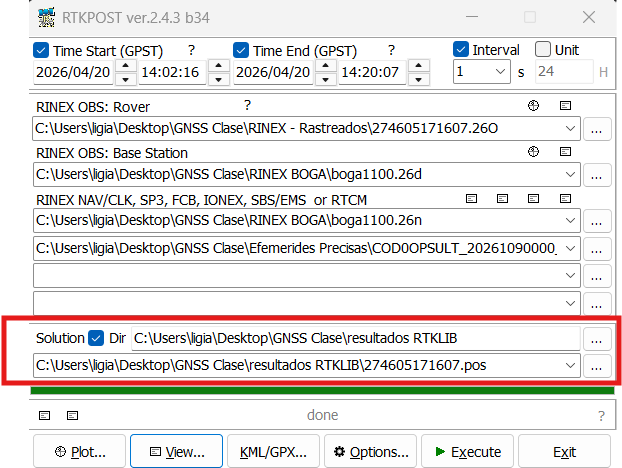
\includegraphics{./53-practica_13_gnss_allynav_r26_files/RTKLIB6.png}

}

\caption{Configuración de Ruta a guardar resultados}

\end{figure}%

\textbf{Configuración del modo de posicionamiento} Luego de cargar los
archivos de entrada, se ingresa al botón \textbf{Options}. En la pestaña
\textbf{Setting1} se configura el modo general del procesamiento.

\begin{figure}[H]

{\centering 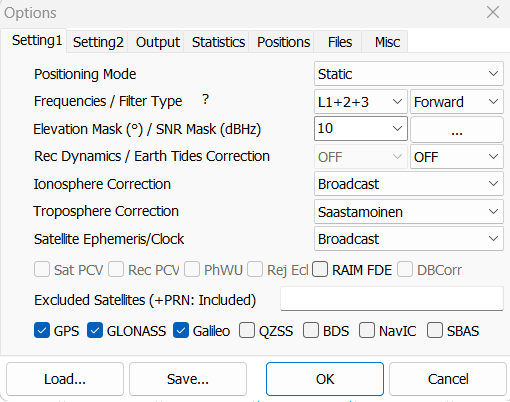
\includegraphics{./53-practica_13_gnss_allynav_r26_files/RTKLIB7.png}

}

\caption{Configuración opciones Setting1}

\end{figure}%

Para esta práctica se selecciona el modo de posicionamiento
\textbf{Static}, dado que se está procesando una ocupación estática
sobre un punto fijo. En el campo \textbf{Frequencies / Filter Type} se
seleccionan las frecuencias disponibles del receptor GNSS utilizadas
durante el rastreo. En este caso se emplea la opción \textbf{L1+2+3}.

La máscara de elevación se configura en \textbf{10°}, valor que debe
coincidir con la máscara utilizada durante la medición en campo. En
cuanto a las constelaciones, se seleccionan \textbf{GPS},
\textbf{GLONASS} y \textbf{Galileo}, correspondientes a las señales que
se desean considerar en el procesamiento.

En esta misma pestaña se mantienen las siguientes opciones generales:

\begin{longtable}[]{@{}ll@{}}
\toprule\noalign{}
Parámetro & Configuración usada \\
\midrule\noalign{}
\endhead
\bottomrule\noalign{}
\endlastfoot
Positioning Mode & Static \\
Frequencies / Filter Type & L1+2+3 \\
Elevation Mask & 10° \\
Ionosphere Correction & Broadcast \\
Troposphere Correction & Saastamoinen \\
Satellite Ephemeris/Clock & Broadcast \\
Constelaciones & GPS, GLONASS y Galileo \\
\end{longtable}

\textbf{Configuración de ambigüedades} En la pestaña \textbf{Setting2}
se revisan los parámetros asociados a la resolución de ambigüedades.
Para esta práctica no se realizaron modificaciones respecto a la
configuración por defecto.

Se mantiene la resolución de ambigüedades en modo continuo, con la
opción correspondiente activada. Esta configuración permite que el
programa gestione la resolución de ambigüedades durante el procesamiento
de la línea base.

\begin{figure}[H]

{\centering 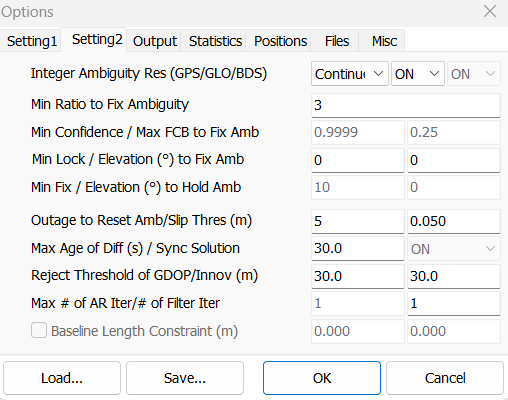
\includegraphics{./53-practica_13_gnss_allynav_r26_files/RTKLIB8.png}

}

\caption{Configuración opciones Setting2}

\end{figure}%

\textbf{Configuración del formato de salida} En la pestaña
\textbf{Output} se define el formato de los resultados. Para esta
práctica se selecciona como formato de solución \textbf{Lat/Lon/Height},
con el fin de obtener las coordenadas finales en latitud, longitud y
altura.

El formato de tiempo se deja en \textbf{hh:mm:ss GPST}, y el formato de
latitud y longitud se define en \textbf{grados decimales}. El datum se
configura como \textbf{WGS84} y la altura se mantiene como
\textbf{elipsoidal}.

Es importante cambiar la opción \textbf{Solution for Static Mode} a
\textbf{Single}, de manera que el procesamiento entregue una única
coordenada final para el punto observado.

\begin{figure}[H]

{\centering 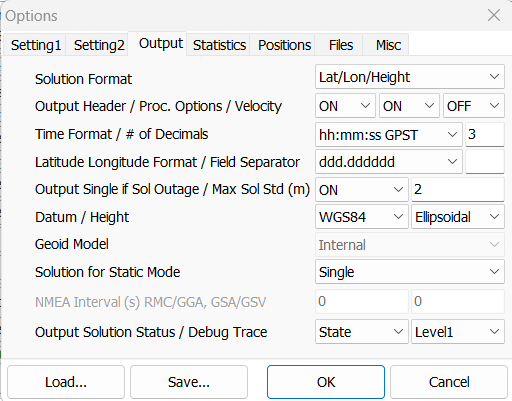
\includegraphics{./53-practica_13_gnss_allynav_r26_files/RTKLIB9.png}

}

\caption{Configuración del formato de salida, datum, altura elipsoidal y
solución estática única}

\end{figure}%

La configuración usada en esta pestaña se resume así:

\begin{longtable}[]{@{}ll@{}}
\toprule\noalign{}
Parámetro & Configuración usada \\
\midrule\noalign{}
\endhead
\bottomrule\noalign{}
\endlastfoot
Solution Format & Lat/Lon/Height \\
Time Format & hh:mm:ss GPST \\
Latitude/Longitude Format & Grados decimales \\
Datum & WGS84 \\
Height & Ellipsoidal \\
Solution for Static Mode & Single \\
\end{longtable}

\textbf{Parámetros estadísticos} En la pestaña \textbf{Statistics} se
revisan los parámetros estadísticos asociados al procesamiento. Para
esta práctica no se realizaron modificaciones en esta sección,
conservando los valores definidos por defecto en RTKPOST.

\begin{figure}[H]

{\centering 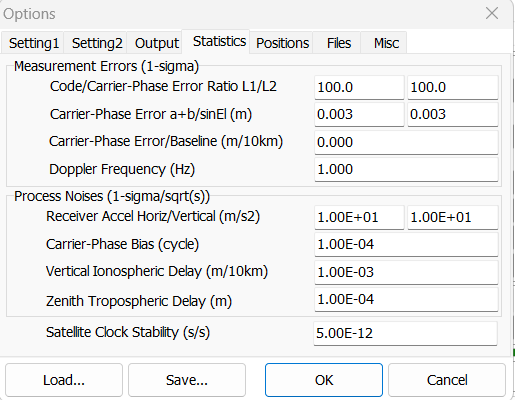
\includegraphics{./53-practica_13_gnss_allynav_r26_files/RTKLIB10.png}

}

\caption{Parámetros estadísticos conservados por defecto en RTKPOST}

\end{figure}%

\textbf{Configuración de posiciones y alturas de antena} En la pestaña
\textbf{Positions} se configuran las posiciones del rover y de la
estación base. Para el caso de esta práctica, el \textbf{rover}
corresponde al punto observado sobre el vértice geodésico, mientras que
la \textbf{Base Station} corresponde a la estación permanente
\textbf{BOGA} del IGAC.

En el campo del rover se debe ingresar la altura de antena medida
durante la práctica, correspondiente a la distancia entre el punto
físico ocupado y la marca de referencia del receptor. Es fundamental
verificar si la altura fue medida de forma vertical o inclinada, ya que
este dato influye directamente en la altura final del punto procesado.

En la sección \textbf{Base Station} se ingresan las coordenadas
oficiales de la estación BOGA, descargadas desde la página de la Red
Geodésica del IGAC. También se debe ingresar la altura de antena
correspondiente a dicha estación, de acuerdo con la información
disponible para la fecha del levantamiento.

\begin{figure}[H]

{\centering 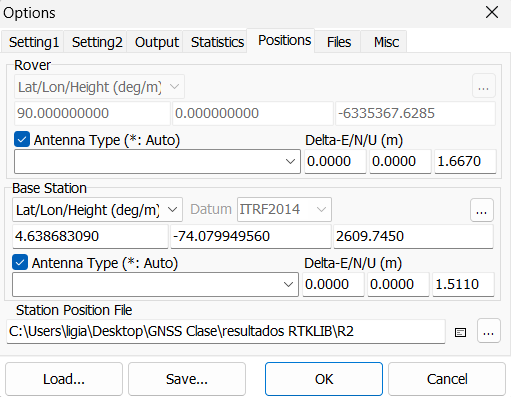
\includegraphics{./53-practica_13_gnss_allynav_r26_files/RTKLIB11.png}

}

\caption{Configuración de coordenadas de la estación BOGA y alturas de
antena}

\end{figure}%

Para esta práctica se emplearon como referencia las coordenadas de la
estación BOGA en latitud, longitud y altura elipsoidal. Una vez
ingresada esta información, se selecciona la carpeta o archivo donde se
almacenarán los resultados del procesamiento.

\textbf{Ejecución del postproceso} Después de configurar los archivos de
entrada, el intervalo temporal, las opciones de procesamiento, el
formato de salida y las posiciones de referencia, se regresa a la
ventana principal de RTKPOST y se presiona el botón \textbf{Execute}.

El programa ejecuta el procesamiento y, al finalizar, muestra la barra
de progreso completa con el mensaje \textbf{done}. Esto indica que el
archivo de resultados fue generado correctamente en la ruta definida.

\begin{figure}[H]

{\centering 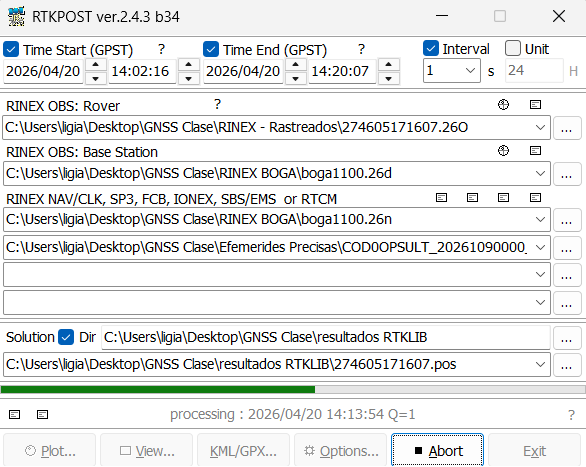
\includegraphics{./53-practica_13_gnss_allynav_r26_files/RTKLIB12.png}

}

\caption{Ejecución del postproceso en RTKPOST y generación del archivo
POS}

\end{figure}%

\textbf{Revisión de resultados} Finalizado el procesamiento, se abre el
archivo \texttt{.pos} generado por RTKPOST. Este archivo contiene el
resumen del procesamiento, los archivos utilizados, el intervalo de
observación, el modo de posicionamiento, las constelaciones empleadas,
las opciones de corrección y la coordenada resultante.

En los resultados se debe revisar la coordenada final obtenida para el
punto observado, así como los indicadores de calidad del procesamiento.
Entre los parámetros más importantes se encuentran:

\begin{longtable}[]{@{}ll@{}}
\toprule\noalign{}
Parámetro & Descripción \\
\midrule\noalign{}
\endhead
\bottomrule\noalign{}
\endlastfoot
Latitude & Latitud final del punto observado \\
Longitude & Longitud final del punto observado \\
Height & Altura elipsoidal final \\
Q & Calidad de la solución \\
ns & Número de satélites utilizados \\
sdn, sde, sdu & Desviaciones estándar en norte, este y altura \\
ratio & Indicador asociado a la solución de ambigüedades \\
\end{longtable}

En RTKPOST, el campo \textbf{Q} permite identificar el tipo de solución
obtenida. De acuerdo con la leyenda del archivo de resultados, los
valores más comunes son:

\begin{longtable}[]{@{}ll@{}}
\toprule\noalign{}
Valor Q & Tipo de solución \\
\midrule\noalign{}
\endhead
\bottomrule\noalign{}
\endlastfoot
1 & Fija \\
2 & Flotante \\
5 & Simple \\
\end{longtable}

Para esta práctica, el archivo de salida permite visualizar las
coordenadas finales del punto observado y la calidad de la solución
obtenida. Estos valores serán utilizados posteriormente para comparar la
coordenada postprocesada de la base con la coordenada utilizada en campo
durante el levantamiento RTK.

\begin{figure}[H]

{\centering 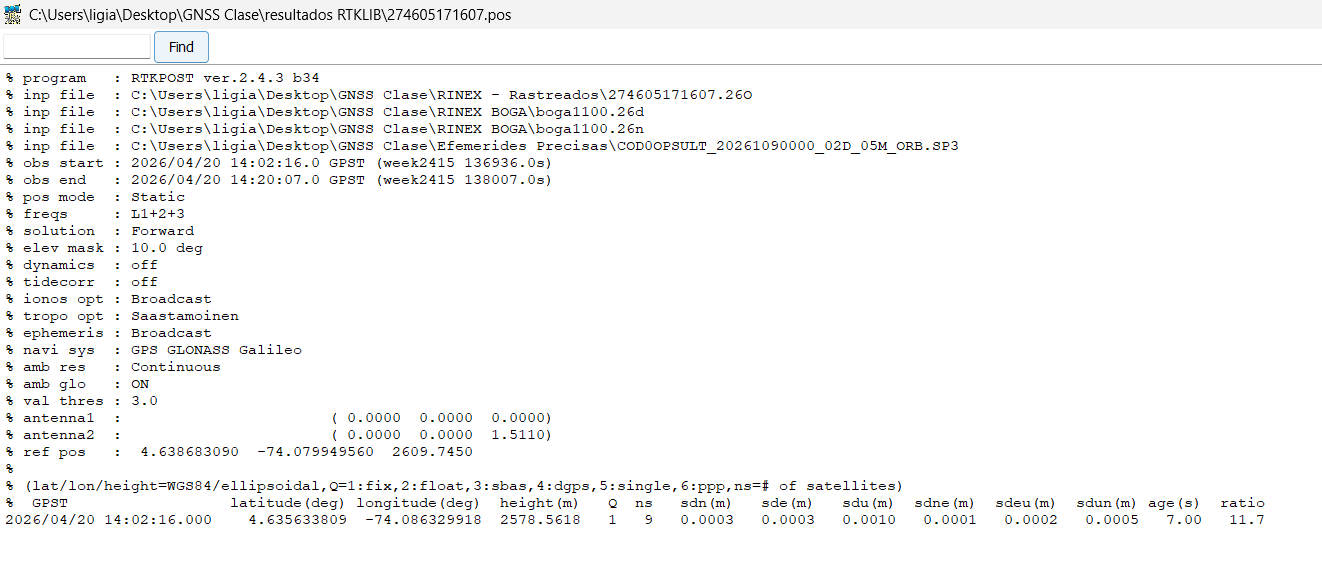
\includegraphics{./53-practica_13_gnss_allynav_r26_files/RTKLIB0.png}

}

\caption{Visualización del archivo POS con coordenadas finales y calidad
de la solución}

\end{figure}%

La coordenada obtenida mediante RTKPOST corresponde a la coordenada
ajustada del punto observado durante el levantamiento estático. Esta
coordenada debe compararse con la coordenada inicialmente utilizada para
configurar la estación base durante el levantamiento RTK.

Si existe una diferencia entre ambas coordenadas, se calcula el
desplazamiento en Este, Norte y altura. Posteriormente, dicho
desplazamiento puede aplicarse a los puntos levantados en modo
cinemático RTK, con el fin de mejorar el amarre absoluto del
levantamiento al sistema de referencia utilizado.

En síntesis, el postproceso con RTKPOST permite:

\begin{longtable}[]{@{}
  >{\raggedright\arraybackslash}p{(\columnwidth - 2\tabcolsep) * \real{0.5000}}
  >{\raggedright\arraybackslash}p{(\columnwidth - 2\tabcolsep) * \real{0.5000}}@{}}
\toprule\noalign{}
\begin{minipage}[b]{\linewidth}\raggedright
Resultado
\end{minipage} & \begin{minipage}[b]{\linewidth}\raggedright
Utilidad
\end{minipage} \\
\midrule\noalign{}
\endhead
\bottomrule\noalign{}
\endlastfoot
Obtener la coordenada final de la base & Sirve como coordenada corregida
del punto ocupado \\
Revisar la calidad de la solución & Permite evaluar si el procesamiento
fue fijo, flotante o simple \\
Comparar contra la coordenada usada en campo & Permite identificar
desplazamientos \\
Corregir el levantamiento RTK & Permite trasladar los puntos rover según
el ajuste de la base \\
\end{longtable}

\subsubsection{Resultados de los postprocesos realizados con las
diferentes
aplicaciones}\label{resultados-de-los-postprocesos-realizados-con-las-diferentes-aplicaciones}

Como resultado del postproceso se obtiene una coordenada final para el
punto observado durante el levantamiento estático. Esta coordenada debe
revisarse junto con los indicadores de calidad reportados por el
software, tales como precisión estimada, tipo de solución, residuos,
número de satélites utilizados y consistencia general del procesamiento.

La coordenada obtenida mediante postproceso debe compararse con la
coordenada que fue utilizada inicialmente para configurar la estación
base durante el levantamiento RTK. Esta comparación permite determinar
si existe un desplazamiento en Este, Norte y altura.

\subsubsection{Con Emlid Studio}\label{con-emlid-studio}

La solución resultado de este postproceso fue single (5) significa que
no fue precisa. ``Revisar''

\begin{figure}[H]

{\centering 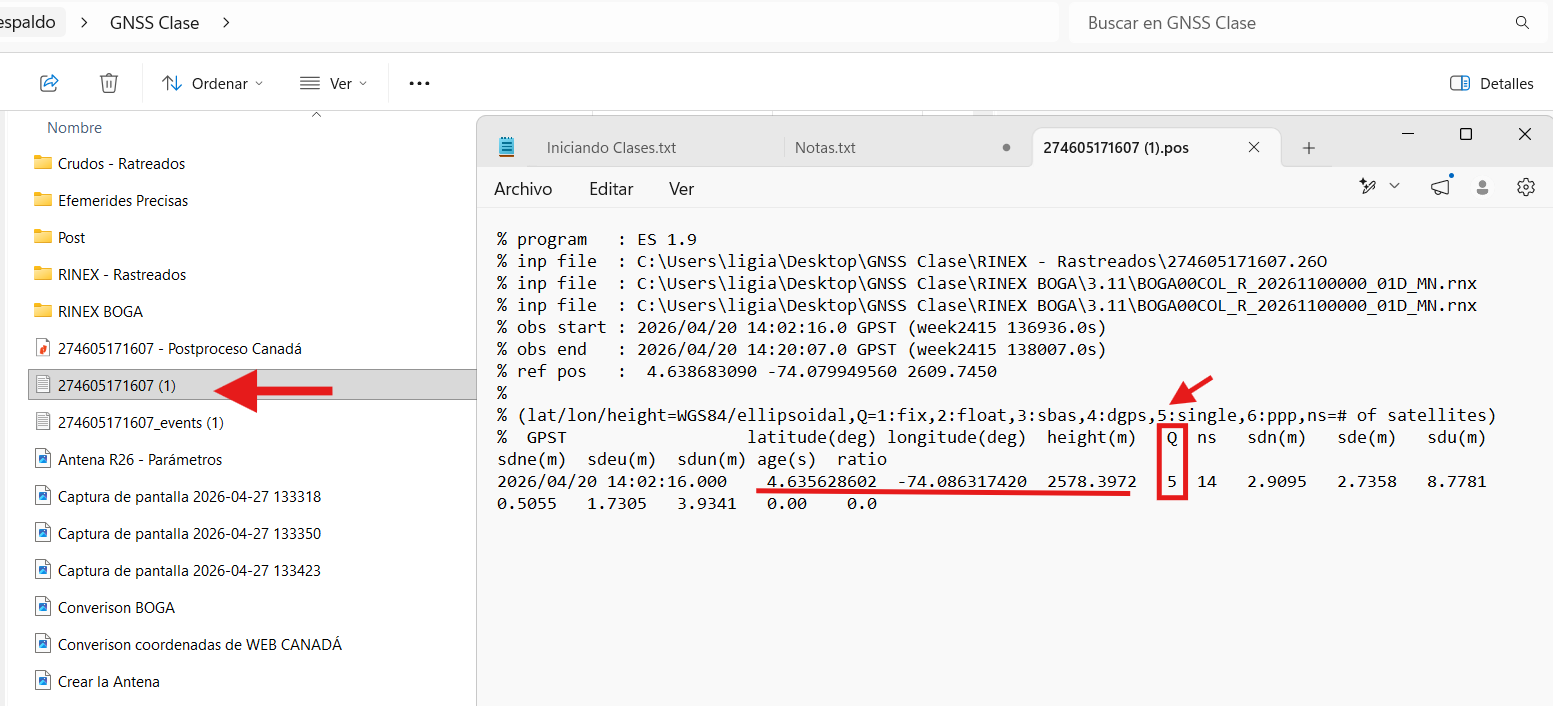
\includegraphics{./53-practica_13_gnss_allynav_r26_files/Emlid13.png}

}

\caption{Resultados del postproceso con EMLID STUDIO: coordenadas
finales de la base}

\end{figure}%

A continuación se presentan las coordenadas obtenidas según el archivo
de registro procesado con EMLID STUDIO:

\begin{longtable}[]{@{}
  >{\centering\arraybackslash}p{(\columnwidth - 8\tabcolsep) * \real{0.2000}}
  >{\centering\arraybackslash}p{(\columnwidth - 8\tabcolsep) * \real{0.2000}}
  >{\centering\arraybackslash}p{(\columnwidth - 8\tabcolsep) * \real{0.2000}}
  >{\centering\arraybackslash}p{(\columnwidth - 8\tabcolsep) * \real{0.2000}}
  >{\centering\arraybackslash}p{(\columnwidth - 8\tabcolsep) * \real{0.2000}}@{}}
\caption{Coordenadas extraídas del archivo 274605171607
(1).pos}\label{tbl-gnss-results}\tabularnewline
\toprule\noalign{}
\begin{minipage}[b]{\linewidth}\centering
Latitud (deg)
\end{minipage} & \begin{minipage}[b]{\linewidth}\centering
Longitud (deg)
\end{minipage} & \begin{minipage}[b]{\linewidth}\centering
Altura Elipsoidal (m)
\end{minipage} & \begin{minipage}[b]{\linewidth}\centering
Calidad (Q)
\end{minipage} & \begin{minipage}[b]{\linewidth}\centering
Satélites (ns)
\end{minipage} \\
\midrule\noalign{}
\endfirsthead
\toprule\noalign{}
\begin{minipage}[b]{\linewidth}\centering
Latitud (deg)
\end{minipage} & \begin{minipage}[b]{\linewidth}\centering
Longitud (deg)
\end{minipage} & \begin{minipage}[b]{\linewidth}\centering
Altura Elipsoidal (m)
\end{minipage} & \begin{minipage}[b]{\linewidth}\centering
Calidad (Q)
\end{minipage} & \begin{minipage}[b]{\linewidth}\centering
Satélites (ns)
\end{minipage} \\
\midrule\noalign{}
\endhead
\bottomrule\noalign{}
\endlastfoot
4.635628602 & -74.086317420 & 2578.3972 & 5 (Single) & 14 \\
\end{longtable}

\begin{itemize}
\tightlist
\item
  Precisiones Estimadas (Desviación Estándar)
\end{itemize}

\begin{longtable}[]{@{}lc@{}}
\caption{Errores estándar del
posicionamiento}\label{tbl-precision}\tabularnewline
\toprule\noalign{}
Componente & Valor (m) \\
\midrule\noalign{}
\endfirsthead
\toprule\noalign{}
Componente & Valor (m) \\
\midrule\noalign{}
\endhead
\bottomrule\noalign{}
\endlastfoot
Norte (sdn) & 2.9095 \\
Este (sde) & 2.7358 \\
Vertical (sdu) & 8.7781 \\
\end{longtable}

\subsubsection{Con RTKLIB}\label{con-rtklib}

Se obtuvo una solución \textbf{estática fija (Fix)} mediante RTKPOST,
procesando el archivo de observación del punto levantado contra la
estación permanente \textbf{BOGA} del IGAC. En el procesamiento se
cargaron los archivos RINEX de observación, navegación y el archivo de
efemérides precisas (\texttt{.sp3}). No obstante, en la configuración
mostrada, RTKPOST reporta el uso de efemérides en modo
\textbf{Broadcast}, por lo cual debe verificarse en las opciones del
procesamiento que las efemérides precisas hayan sido efectivamente
empleadas.

Coordenadas geodésicas obtenidas en WGS84, con altura elipsoidal:

\begin{longtable}[]{@{}lc@{}}
\caption{Coordenadas finales obtenidas mediante
RTKPOST}\label{tbl-fix-results}\tabularnewline
\toprule\noalign{}
Parámetro & Valor obtenido \\
\midrule\noalign{}
\endfirsthead
\toprule\noalign{}
Parámetro & Valor obtenido \\
\midrule\noalign{}
\endhead
\bottomrule\noalign{}
\endlastfoot
\textbf{Latitud} & 4.635633809° \\
\textbf{Longitud} & -74.086329918° \\
\textbf{Altura elipsoidal} & 2576.8939 m \\
\textbf{Calidad (Q)} & 1 (Fix) \\
\textbf{Satélites (ns)} & 9 \\
\end{longtable}

Indicadores de calidad y precisión:

La solución presenta una condición favorable de procesamiento,
evidenciada por la obtención de solución fija, desviaciones estándar
reducidas y un valor de \textbf{Ratio} superior al umbral mínimo
configurado de 3.0.

\begin{longtable}[]{@{}lc@{}}
\caption{Indicadores de calidad de la solución
RTKPOST}\label{tbl-rtklib-quality}\tabularnewline
\toprule\noalign{}
Componente & Desviación estándar (m) \\
\midrule\noalign{}
\endfirsthead
\toprule\noalign{}
Componente & Desviación estándar (m) \\
\midrule\noalign{}
\endhead
\bottomrule\noalign{}
\endlastfoot
\textbf{Norte (sdn)} & 0.0003 \\
\textbf{Este (sde)} & 0.0003 \\
\textbf{Vertical (sdu)} & 0.0010 \\
\textbf{Este-Norte (sdne)} & 0.0001 \\
\textbf{Este-Vertical (sdeu)} & 0.0002 \\
\textbf{Vertical-Norte (sdun)} & 0.0005 \\
\textbf{Edad de corrección (age)} & 7.00 s \\
\textbf{Ratio Test} & 11.6 \\
\end{longtable}

\begin{figure}[H]

{\centering 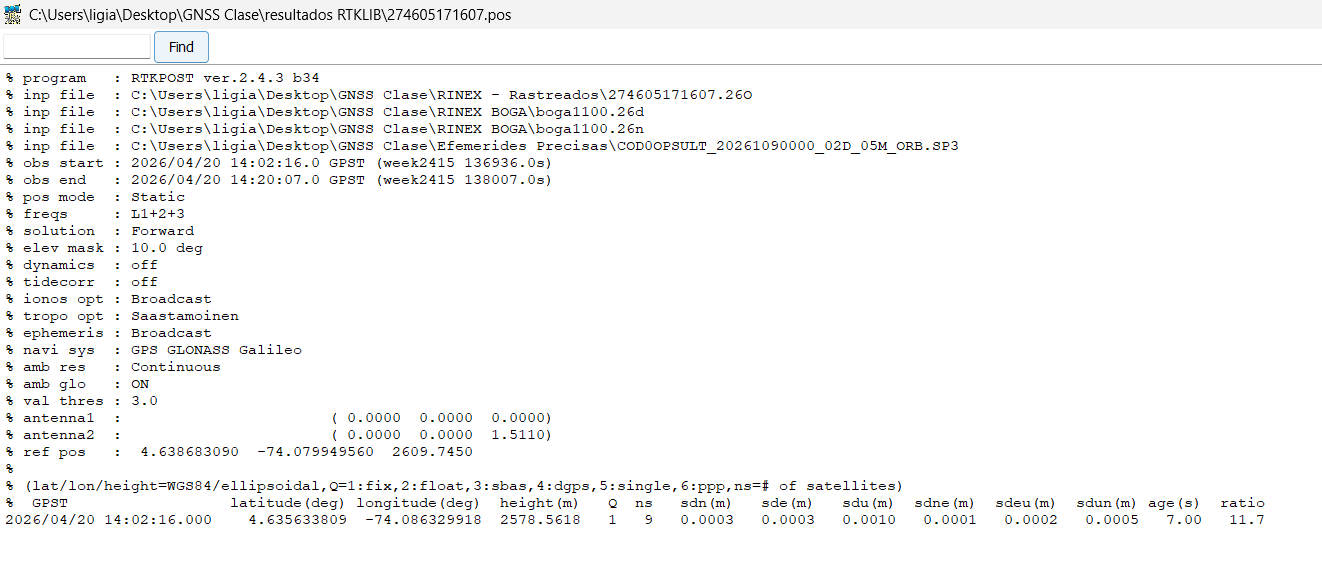
\includegraphics{./53-practica_13_gnss_allynav_r26_files/RTKLIB0.png}

}

\caption{Resultados del postproceso con RTKLIB}

\end{figure}%

\subsubsection{Corrección del levantamiento cinemático
RTK}\label{correcciuxf3n-del-levantamiento-cinemuxe1tico-rtk}

Una vez obtenida la coordenada postprocesada de la base, se puede
revisar el levantamiento cinemático RTK. Debido a que los puntos del
borde de vía fueron levantados tomando como referencia la base instalada
en campo, cualquier desplazamiento identificado en la coordenada de la
base puede trasladarse a los puntos RTK.

En términos generales, la corrección consiste en calcular la diferencia
entre la coordenada inicial de la base y la coordenada postprocesada, y
aplicar ese desplazamiento a las coordenadas de los puntos levantados
con el rover.

\subsection{Síntesis del flujo de
trabajo}\label{suxedntesis-del-flujo-de-trabajo}

El flujo general del postproceso desarrollado en la práctica se resume
de la siguiente manera:

\begin{longtable}[]{@{}
  >{\raggedright\arraybackslash}p{(\columnwidth - 2\tabcolsep) * \real{0.5000}}
  >{\raggedright\arraybackslash}p{(\columnwidth - 2\tabcolsep) * \real{0.5000}}@{}}
\toprule\noalign{}
\begin{minipage}[b]{\linewidth}\raggedright
Etapa
\end{minipage} & \begin{minipage}[b]{\linewidth}\raggedright
Descripción
\end{minipage} \\
\midrule\noalign{}
\endhead
\bottomrule\noalign{}
\endlastfoot
1. Organización de información & Separar archivos del levantamiento
estático, archivos RINEX, datos crudos, archivos de navegación,
efemérides y archivos RTK exportados desde AllyPad \\
2. Conversión a RINEX & Convertir el archivo TXT del receptor a formato
RINEX mediante NovAtel Convert \\
3. Descarga de estación permanente & Descargar los archivos RINEX de la
estación permanente BOGA del IGAC para la misma fecha del
levantamiento \\
4. Descarga de efemérides & Descargar efemérides precisas
correspondientes a la semana GNSS y día del levantamiento \\
5. Procesamiento estático & Procesar la ocupación estática de la base en
Emlid Studio y RTKPOST \\
6. Obtención de coordenada corregida & Obtener la coordenada
postprocesada de la base y revisar su precisión \\
7. Comparación de base & Comparar la coordenada usada en campo con la
coordenada obtenida mediante postproceso \\
8. Corrección RTK & Aplicar el desplazamiento de la base a los puntos
levantados en modo cinemático \\
9. Revisión final & Verificar coordenadas, alturas, descripciones,
precisión reportada y consistencia espacial de los puntos levantados \\
\end{longtable}

\subsection{Recomendaciones/recursos adicionales para el
postproceso}\label{recomendacionesrecursos-adicionales-para-el-postproceso}

\begin{itemize}
\item
  Uso del software
  \href{https://leica-geosystems.com/es-es/rugbycl/archive-data/software/leica-geo-office}{Leica
  Geo Office} (licenciado)
\item
  \textbf{RTKLIB} es un paquete de software libre y de código abierto
  diseñado para el posicionamiento preciso mediante sistemas globales de
  navegación por satélite (GNSS), como GPS, GLONASS, Galileo, BeiDou y
  QZSS. Permite procesar datos en tiempo real (RTK) o postprocesamiento
  (PPK) para obtener precisiones centimétricas, siendo ampliamente
  utilizado en topografía, drones y agricultura de precisió
\item
  Página para identificar la fecha GNSS del levantamiento:
  \url{https://gnsscalendar.com/}
\item
  https://redgeodesica.igac.gov.co/red\_activa.html
\end{itemize}

\section{Actividad final: comparación de resultados y corrección del
levantamiento
RTK}\label{actividad-final-comparaciuxf3n-de-resultados-y-correcciuxf3n-del-levantamiento-rtk}

Como actividad final de la práctica, el estudiante deberá comparar los
resultados obtenidos mediante los diferentes procedimientos de
postproceso y analizar su relación con las coordenadas oficiales del
vértice geodésico observado. Adicionalmente, deberá corregir el
levantamiento cinemático RTK del borde de vía con base en las
coordenadas oficiales del vértice, representarlo sobre un mapa base y
comentar la precisión del levantamiento.

\subsection{Objetivo de la actividad}\label{objetivo-de-la-actividad}

Comparar las coordenadas proyectadas planas obtenidas mediante
diferentes herramientas de postproceso GNSS, contrastarlas con las
coordenadas oficiales del vértice observado y aplicar una corrección al
levantamiento cinemático RTK a partir del desplazamiento identificado en
la estación base.

\subsection{Información que debe utilizar el
estudiante}\label{informaciuxf3n-que-debe-utilizar-el-estudiante}

Para desarrollar la actividad, el estudiante deberá utilizar como mínimo
la siguiente información:

\begin{itemize}
\tightlist
\item
  Coordenadas oficiales del vértice geodésico observado.
\item
  Coordenadas obtenidas mediante postproceso en \textbf{Emlid Studio}.
\item
  Coordenadas obtenidas mediante postproceso en \textbf{RTKLIB /
  RTKPOST}.
\item
  Coordenadas obtenidas mediante el servicio canadiense
  \textbf{CSRS-PPP}.
\item
  Coordenadas del levantamiento cinemático RTK exportadas desde el
  colector de datos.
\item
  Coordenadas utilizadas en campo para configurar la estación base RTK.
\end{itemize}

El servicio canadiense \textbf{CSRS-PPP} puede consultarse en el
siguiente enlace:

\url{https://webapp.csrs-scrs.nrcan-rncan.gc.ca/geod/account-compte/login.php}

Como soporte de la actividad, se deberá incluir una imagen o tabla con
las coordenadas oficiales del vértice geodésico observado.

\begin{figure}[H]

{\centering \includegraphics{./53-practica_13_gnss_allynav_r26_files/coordenadas_oficiales_vertice.png}

}

\caption{Coordenadas oficiales del vértice geodésico observado}

\end{figure}%

\subsection{Parte 1. Comparación de coordenadas
proyectadas}\label{parte-1.-comparaciuxf3n-de-coordenadas-proyectadas}

El estudiante deberá proyectar a coordenadas planas los resultados
obtenidos en los diferentes postprocesos. Para esta práctica se
recomienda trabajar en el sistema \textbf{MAGNA-SIRGAS / Origen
Nacional}, salvo que el docente indique otro sistema de referencia.

Una vez proyectadas las coordenadas, se deberá completar la siguiente
tabla:

\begin{longtable}[]{@{}
  >{\raggedright\arraybackslash}p{(\columnwidth - 14\tabcolsep) * \real{0.1000}}
  >{\raggedleft\arraybackslash}p{(\columnwidth - 14\tabcolsep) * \real{0.1333}}
  >{\raggedleft\arraybackslash}p{(\columnwidth - 14\tabcolsep) * \real{0.1333}}
  >{\raggedleft\arraybackslash}p{(\columnwidth - 14\tabcolsep) * \real{0.1333}}
  >{\raggedleft\arraybackslash}p{(\columnwidth - 14\tabcolsep) * \real{0.1333}}
  >{\raggedleft\arraybackslash}p{(\columnwidth - 14\tabcolsep) * \real{0.1333}}
  >{\raggedleft\arraybackslash}p{(\columnwidth - 14\tabcolsep) * \real{0.1333}}
  >{\raggedright\arraybackslash}p{(\columnwidth - 14\tabcolsep) * \real{0.1000}}@{}}
\caption{Tabla para comparación de coordenadas proyectadas del vértice
observado}\label{tbl-comparacion-postprocesos}\tabularnewline
\toprule\noalign{}
\begin{minipage}[b]{\linewidth}\raggedright
Fuente del resultado
\end{minipage} & \begin{minipage}[b]{\linewidth}\raggedleft
Este (m)
\end{minipage} & \begin{minipage}[b]{\linewidth}\raggedleft
Norte (m)
\end{minipage} & \begin{minipage}[b]{\linewidth}\raggedleft
Altura (m)
\end{minipage} & \begin{minipage}[b]{\linewidth}\raggedleft
Δ Este (m)
\end{minipage} & \begin{minipage}[b]{\linewidth}\raggedleft
Δ Norte (m)
\end{minipage} & \begin{minipage}[b]{\linewidth}\raggedleft
Δ Altura (m)
\end{minipage} & \begin{minipage}[b]{\linewidth}\raggedright
Observación
\end{minipage} \\
\midrule\noalign{}
\endfirsthead
\toprule\noalign{}
\begin{minipage}[b]{\linewidth}\raggedright
Fuente del resultado
\end{minipage} & \begin{minipage}[b]{\linewidth}\raggedleft
Este (m)
\end{minipage} & \begin{minipage}[b]{\linewidth}\raggedleft
Norte (m)
\end{minipage} & \begin{minipage}[b]{\linewidth}\raggedleft
Altura (m)
\end{minipage} & \begin{minipage}[b]{\linewidth}\raggedleft
Δ Este (m)
\end{minipage} & \begin{minipage}[b]{\linewidth}\raggedleft
Δ Norte (m)
\end{minipage} & \begin{minipage}[b]{\linewidth}\raggedleft
Δ Altura (m)
\end{minipage} & \begin{minipage}[b]{\linewidth}\raggedright
Observación
\end{minipage} \\
\midrule\noalign{}
\endhead
\bottomrule\noalign{}
\endlastfoot
Coordenada oficial del vértice & & & & 0.000 & 0.000 & 0.000 &
Coordenada de referencia \\
Emlid Studio & & & & & & & Indicar calidad de solución \\
RTKLIB / RTKPOST & & & & & & & Indicar si fue Fix, Float o Single \\
CSRS-PPP Canadá & & & & & & & Resultado del servicio web \\
Otro procesamiento & & & & & & & Opcional \\
\end{longtable}

Las diferencias deberán calcularse respecto a la coordenada oficial del
vértice:

\[
\Delta E = E_{postproceso} - E_{oficial}
\]

\[
\Delta N = N_{postproceso} - N_{oficial}
\]

\[
\Delta H = H_{postproceso} - H_{oficial}
\]

Donde:

\begin{itemize}
\tightlist
\item
  \(\Delta E\) corresponde a la diferencia en coordenada Este.
\item
  \(\Delta N\) corresponde a la diferencia en coordenada Norte.
\item
  \(\Delta H\) corresponde a la diferencia en altura.
\item
  \(E_{oficial}\), \(N_{oficial}\) y \(H_{oficial}\) corresponden a las
  coordenadas oficiales del vértice observado.
\end{itemize}

\subsection{Parte 2. Cálculo del error
horizontal}\label{parte-2.-cuxe1lculo-del-error-horizontal}

Con base en las diferencias calculadas, el estudiante deberá estimar el
error horizontal de cada resultado de postproceso mediante la siguiente
expresión:

\[
e_h = \sqrt{(\Delta E)^2 + (\Delta N)^2}
\]

Luego, deberá completar la siguiente tabla:

\begin{longtable}[]{@{}
  >{\raggedright\arraybackslash}p{(\columnwidth - 10\tabcolsep) * \real{0.1364}}
  >{\raggedleft\arraybackslash}p{(\columnwidth - 10\tabcolsep) * \real{0.1818}}
  >{\raggedleft\arraybackslash}p{(\columnwidth - 10\tabcolsep) * \real{0.1818}}
  >{\raggedleft\arraybackslash}p{(\columnwidth - 10\tabcolsep) * \real{0.1818}}
  >{\raggedleft\arraybackslash}p{(\columnwidth - 10\tabcolsep) * \real{0.1818}}
  >{\raggedright\arraybackslash}p{(\columnwidth - 10\tabcolsep) * \real{0.1364}}@{}}
\caption{Tabla para resumen de errores respecto a la coordenada
oficial}\label{tbl-errores-postprocesos}\tabularnewline
\toprule\noalign{}
\begin{minipage}[b]{\linewidth}\raggedright
Fuente del resultado
\end{minipage} & \begin{minipage}[b]{\linewidth}\raggedleft
Δ Este (m)
\end{minipage} & \begin{minipage}[b]{\linewidth}\raggedleft
Δ Norte (m)
\end{minipage} & \begin{minipage}[b]{\linewidth}\raggedleft
Error horizontal \(e_h\) (m)
\end{minipage} & \begin{minipage}[b]{\linewidth}\raggedleft
Δ Altura (m)
\end{minipage} & \begin{minipage}[b]{\linewidth}\raggedright
Comentario
\end{minipage} \\
\midrule\noalign{}
\endfirsthead
\toprule\noalign{}
\begin{minipage}[b]{\linewidth}\raggedright
Fuente del resultado
\end{minipage} & \begin{minipage}[b]{\linewidth}\raggedleft
Δ Este (m)
\end{minipage} & \begin{minipage}[b]{\linewidth}\raggedleft
Δ Norte (m)
\end{minipage} & \begin{minipage}[b]{\linewidth}\raggedleft
Error horizontal \(e_h\) (m)
\end{minipage} & \begin{minipage}[b]{\linewidth}\raggedleft
Δ Altura (m)
\end{minipage} & \begin{minipage}[b]{\linewidth}\raggedright
Comentario
\end{minipage} \\
\midrule\noalign{}
\endhead
\bottomrule\noalign{}
\endlastfoot
Emlid Studio & & & & & \\
RTKLIB / RTKPOST & & & & & \\
CSRS-PPP Canadá & & & & & \\
Otro procesamiento & & & & & \\
\end{longtable}

El estudiante deberá comentar cuál de los métodos presentó menor
diferencia respecto a la coordenada oficial y si los resultados son
coherentes con la calidad de solución reportada por cada software.

\subsection{Parte 3. Corrección del levantamiento cinemático
RTK}\label{parte-3.-correcciuxf3n-del-levantamiento-cinemuxe1tico-rtk}

Como punto adicional, el estudiante deberá corregir el levantamiento
cinemático RTK del borde de vía tomando como referencia las coordenadas
oficiales del vértice geodésico observado.

Para ello, deberá comparar la coordenada utilizada en campo para
configurar la estación base con la coordenada oficial del vértice. A
partir de esa comparación se obtendrá el desplazamiento que deberá
aplicarse a todos los puntos levantados con el rover.

El desplazamiento de la base se calcula así:

\[
\Delta E_{base} = E_{oficial} - E_{base\_campo}
\]

\[
\Delta N_{base} = N_{oficial} - N_{base\_campo}
\]

\[
\Delta H_{base} = H_{oficial} - H_{base\_campo}
\]

Luego, para cada punto del levantamiento cinemático RTK, se deberán
calcular las coordenadas corregidas:

\[
E_{corr} = E_{RTK} + \Delta E_{base}
\]

\[
N_{corr} = N_{RTK} + \Delta N_{base}
\]

\[
H_{corr} = H_{RTK} + \Delta H_{base}
\]

Donde:

\begin{itemize}
\tightlist
\item
  \(E_{base\_campo}\), \(N_{base\_campo}\) y \(H_{base\_campo}\)
  corresponden a las coordenadas usadas en campo para configurar la
  base.
\item
  \(E_{oficial}\), \(N_{oficial}\) y \(H_{oficial}\) corresponden a las
  coordenadas oficiales del vértice.
\item
  \(E_{RTK}\), \(N_{RTK}\) y \(H_{RTK}\) corresponden a las coordenadas
  originales levantadas con el rover.
\item
  \(E_{corr}\), \(N_{corr}\) y \(H_{corr}\) corresponden a las
  coordenadas corregidas del levantamiento RTK.
\end{itemize}

El estudiante deberá completar una tabla como la siguiente:

\begin{longtable}[]{@{}
  >{\raggedright\arraybackslash}p{(\columnwidth - 14\tabcolsep) * \real{0.1000}}
  >{\raggedleft\arraybackslash}p{(\columnwidth - 14\tabcolsep) * \real{0.1333}}
  >{\raggedleft\arraybackslash}p{(\columnwidth - 14\tabcolsep) * \real{0.1333}}
  >{\raggedleft\arraybackslash}p{(\columnwidth - 14\tabcolsep) * \real{0.1333}}
  >{\raggedleft\arraybackslash}p{(\columnwidth - 14\tabcolsep) * \real{0.1333}}
  >{\raggedleft\arraybackslash}p{(\columnwidth - 14\tabcolsep) * \real{0.1333}}
  >{\raggedleft\arraybackslash}p{(\columnwidth - 14\tabcolsep) * \real{0.1333}}
  >{\raggedright\arraybackslash}p{(\columnwidth - 14\tabcolsep) * \real{0.1000}}@{}}
\caption{Tabla para corrección de puntos levantados mediante
RTK}\label{tbl-correccion-rtk}\tabularnewline
\toprule\noalign{}
\begin{minipage}[b]{\linewidth}\raggedright
Punto
\end{minipage} & \begin{minipage}[b]{\linewidth}\raggedleft
Este RTK (m)
\end{minipage} & \begin{minipage}[b]{\linewidth}\raggedleft
Norte RTK (m)
\end{minipage} & \begin{minipage}[b]{\linewidth}\raggedleft
Altura RTK (m)
\end{minipage} & \begin{minipage}[b]{\linewidth}\raggedleft
Este corregido (m)
\end{minipage} & \begin{minipage}[b]{\linewidth}\raggedleft
Norte corregido (m)
\end{minipage} & \begin{minipage}[b]{\linewidth}\raggedleft
Altura corregida (m)
\end{minipage} & \begin{minipage}[b]{\linewidth}\raggedright
Descripción
\end{minipage} \\
\midrule\noalign{}
\endfirsthead
\toprule\noalign{}
\begin{minipage}[b]{\linewidth}\raggedright
Punto
\end{minipage} & \begin{minipage}[b]{\linewidth}\raggedleft
Este RTK (m)
\end{minipage} & \begin{minipage}[b]{\linewidth}\raggedleft
Norte RTK (m)
\end{minipage} & \begin{minipage}[b]{\linewidth}\raggedleft
Altura RTK (m)
\end{minipage} & \begin{minipage}[b]{\linewidth}\raggedleft
Este corregido (m)
\end{minipage} & \begin{minipage}[b]{\linewidth}\raggedleft
Norte corregido (m)
\end{minipage} & \begin{minipage}[b]{\linewidth}\raggedleft
Altura corregida (m)
\end{minipage} & \begin{minipage}[b]{\linewidth}\raggedright
Descripción
\end{minipage} \\
\midrule\noalign{}
\endhead
\bottomrule\noalign{}
\endlastfoot
P1 & & & & & & & \\
P2 & & & & & & & \\
P3 & & & & & & & \\
P4 & & & & & & & \\
\end{longtable}

\subsection{Parte 4. Representación sobre mapa
base}\label{parte-4.-representaciuxf3n-sobre-mapa-base}

Una vez corregidas las coordenadas del levantamiento cinemático RTK, el
estudiante deberá representar el trazado del borde de vía sobre un mapa
base.

La representación podrá realizarse en un software SIG, como
\textbf{QGIS} o \textbf{ArcGIS}, o mediante una herramienta compatible
con archivos CSV, TXT, KML, GeoJSON o shapefile.

El mapa deberá incluir como mínimo:

\begin{itemize}
\tightlist
\item
  Puntos RTK originales.
\item
  Puntos RTK corregidos.
\item
  Vértice geodésico utilizado como base.
\item
  Mapa base de referencia.
\item
  Sistema de coordenadas empleado.
\item
  Leyenda.
\item
  Escala gráfica.
\item
  Norte.
\item
  Comentario sobre la coherencia espacial del levantamiento.
\end{itemize}

\begin{figure}[H]

{\centering \includegraphics{./53-practica_13_gnss_allynav_r26_files/mapa_base_rtk_corregido.png}

}

\caption{Espacio para mapa base con levantamiento RTK corregido}

\end{figure}%

\subsection{Parte 5. Comentario
técnico}\label{parte-5.-comentario-tuxe9cnico}

Finalmente, el estudiante deberá redactar un comentario técnico breve
sobre la precisión y consistencia del levantamiento realizado.

El comentario deberá responder, como mínimo, las siguientes preguntas:

\begin{itemize}
\tightlist
\item
  ¿Cuál fue la diferencia entre las coordenadas oficiales y las
  coordenadas obtenidas por cada método de postproceso?
\item
  ¿Qué método presentó mejores resultados respecto a la coordenada
  oficial?
\item
  ¿La solución obtenida fue fija, flotante o simple?
\item
  ¿La precisión reportada por el software es coherente con las
  diferencias observadas?
\item
  ¿La corrección aplicada al levantamiento RTK mejoró el amarre absoluto
  de los puntos?
\item
  ¿El levantamiento RTK conserva coherencia geométrica sobre el mapa
  base?
\item
  ¿Qué factores pudieron afectar la precisión del levantamiento?
\end{itemize}

\subsection{Entregables}\label{entregables}

El estudiante deberá entregar los siguientes productos:

\begin{longtable}[]{@{}
  >{\raggedright\arraybackslash}p{(\columnwidth - 2\tabcolsep) * \real{0.5000}}
  >{\raggedright\arraybackslash}p{(\columnwidth - 2\tabcolsep) * \real{0.5000}}@{}}
\caption{Entregables de la actividad
final}\label{tbl-entregables-tarea}\tabularnewline
\toprule\noalign{}
\begin{minipage}[b]{\linewidth}\raggedright
Entregable
\end{minipage} & \begin{minipage}[b]{\linewidth}\raggedright
Descripción
\end{minipage} \\
\midrule\noalign{}
\endfirsthead
\toprule\noalign{}
\begin{minipage}[b]{\linewidth}\raggedright
Entregable
\end{minipage} & \begin{minipage}[b]{\linewidth}\raggedright
Descripción
\end{minipage} \\
\midrule\noalign{}
\endhead
\bottomrule\noalign{}
\endlastfoot
Tabla de comparación de coordenadas & Comparación entre coordenadas
oficiales, Emlid Studio, RTKLIB / RTKPOST, CSRS-PPP y otros
resultados \\
Tabla de errores & Diferencias en Este, Norte, altura y error
horizontal \\
Tabla de corrección RTK & Coordenadas originales y corregidas del
levantamiento cinemático \\
Mapa base & Representación del levantamiento RTK original y corregido \\
Comentario técnico & Análisis de precisión, calidad de solución y
coherencia espacial \\
\end{longtable}



\end{document}
